\chapter{The neutrino}
\label{sec:theory}

\section{A brief history of the neutrino}
\label{sec:theory:history}

\subsection{Direct detection of the neutrino}
\label{sec:theory:history:detection}

% Pauli's hypothesis of the neutrino
The existence of the neutrino as a particle carrying no electric charge was first hypothesised in 1930 by Wolfgang Pauli as a solution to issues observed in the spectrum produced by nuclear $\beta$-decay~\cite{pauliNeutrino}.
At the time, the existence of only 3 year subatomic particles was known, the electron, the proton and the photon~\cite{ideaOfNeutrino}.

In contrast to $\alpha$- and $\gamma$-decay, the energy spectrum of the emitted particle in $\beta$-decay is observed to be continuous~\cite{ideaOfNeutrino}.
Given that $\beta$-decay appeared to be a two-body decay (as $\alpha$- and $\gamma$-decay are) this seemed to violate the principle of conservation of energy.

To rectify this, Pauli proposed the existence of a neutral particle which escaped the nucleus without the detection during $\beta$-decay.
He originally named this particle the ``neutron'', although this name would be used for the neutral baryon after its discovery by Chadwick in 1932~\cite{neutronDiscovery} and the neutrino would instead be known by its modern name.

We now know that an electron neutrino (antineutrino) is emitted during $\beta^{+}$- ($\beta^{-}$-) decay, where the generic equation for the $\beta^{-}$ decay of an atom is
\begin{equation}
  ^{A}_{Z}X~\rightarrow~^{A}_{Z+1}X' + e^{-} + \bar{\nu}_{e} \,,
\end{equation}
where $A$ is the mass number of the atom, and $Z$ is the atomic number. 

% Experimental discovery by Cowan and Reines
Experimental confirmation of the neutrino's existence came in 1956 where the reaction
\begin{equation}
  \bar{\nu}_{e} + p \rightarrow e^{+} + n
  \label{eq:cowanReines}
\end{equation}
was first observed at the Savannah River Plant, South Carolina. The experiment utilised the large neutrino flux from a nuclear reactor incident on the protons in a tank of water sandwiched between scintillation counters.
This water contained a solution of cadmium chloride which emits a photon upon neutron capture.
In the event of the reaction shown in eq.~(\ref{eq:cowanReines}), the outgoing positron would annihilate with an electron in the water, resulting in a prompt coincidence signal.
An additional check was made by requiring a delayed photon from the capture of the outgoing neutron~\cite{cowanReines}.

% Discovery of numu
Up to this point, only electron neutrinos had been observed (counterparts to the electron).
However in 1937 the muon, a heavier counterpart to the electron, was observed~\cite{muonDiscovery}.
In 1962 the existence of a neutrino corresponding to the muon was confirmed at Brookhaven Alternatng Gradient Synchrotron.
These muon neutrinos and antineutrinos ($\nu_{\mu}$ and $\bar{\nu}_{\mu}$) were produced by colliding a beam of protons with a beryllium target, producing charged pions and kaons.
These mesons subsequently decayed via the channels
\begin{align}
    K^{\pm} \rightarrow \mu^{\pm} + \nu_{\mu}(\bar{\nu}_{\mu}) \\
    \pi^{\pm} \rightarrow \mu^{\pm} + \nu_{\mu}(\bar{\nu}_{\mu})
\end{align}
to produce the desired neutrinos and antineutrinos.

The resulting neutrino interactions were then observed in a spark chamber.
Interactions arising from muon neutrinos and antineutrinos were identified by the prescence of one or more long tracks originating from within the fiducial volume of the detector at the same time as the beam pulse~\cite{numuDiscovery}.   

% C. S. Wu's discovery of neutrino helicity and parity violation?

% nutau discovery from DONUT
The discovery of the tau lepton in $e^{+}e^{-}$ collisions in 1975~\cite{tauLepton} led to the theorisation of a corresponding neutrino, in keeping with the two already identified for the electron and muon leptons.
However, due to the high mass of the tau lepton ($1777~\text{MeV}/c^{2}$ compared to $0.5110~\text{MeV}/c^{2}$ and $105.7~\text{MeV}/c^{2}$ for the electron and muon respectively~\cite{pdg2018}) a higher energy beam was required for direct observation of the tau neutrino since the $K^{\pm}$ and $\pi^{\pm}$ mesons typically used in beam neutrino experiments did not have high enough masses to decay to a tau lepton-neutrino pair.

From 1997, the DONuT (Direct Observation of the Nu Tau) collaboration fired a beam of 800~GeV protons from the Tevatron into a tungsten alloy target.
Although this process produced many $\pi^{\pm}$ and $K^{\pm}$ mesons, the centre of mass energy was high enough in this case to produce significant numbers of $D_{s}$ mesons~\cite{donutFinal}.
These $D_{s}$ mesons decay leptonically to $\tau^{+}\nu_{\tau}$ with a branching fraction of 5.48\%~\cite{dsFraction}, producing a flux of tau neutrinos.
In 2000 the collaboration reported the observation of 4 suspected tau neutrino charged current interactions with an estimated background of 0.34 events, thus confirming the tau neutrino's existence~\cite{tauNeutrino}.  

Since this discovery no evidence for further leptons, charged or neutral, has been observed.
Results from the the LEP (Large Electron Positron) collider also indicate that the number of neutrino flavours is 3.
This result was inferred by observing the width of the $Z$ boson using $e^{+}e^{-}$ collisions.
The width of the $Z$ boson, $\Gamma_{Z}$ is given as
\begin{equation}
  \Gamma_{Z} = \Gamma_{ee} + \Gamma_{\mu\mu} + \Gamma_{\tau\tau} + \Gamma_{\text{hadrons}} + N_{\nu}\Gamma_{\nu\nu}
\end{equation}
where the various terms are the partial decay widths of the $Z$ boson into various particles and $N_{\nu}$ is the number of neutrino flavours.
These partial decay widths can be calculated from Z-boson couplings and standard model parameters.
By precisely measuring both $m_{Z}$ and $\Gamma_{Z}$ it was determined that $N_{\nu} = 2.9840 \pm 0.0082$, confirming that only 3 flavours of neutrino exist for $m_{\nu} < m_{Z}/2$~\cite{zBosonWidth}.
One such plot showing combined measurements from the various LEP experiments is shown in Figure~\ref{fig:zBosonWidth}, clearly showing the preference of the data for the three neutrino case.

\begin{figure}[h]
  \centering
  \includegraphics[width=.5\linewidth]{files/figures/theory/zBosonWidth}
  \caption{From~\cite{zBosonWidth}, this plot shows the hadron production cross-section as a function of centre of mass energy around the $Z$ boson resonance. The data are from the four LEP experiments and are shown as the points. It can clearly be seen that the data prefers the three neutrino case.}
  \label{fig:zBosonWidth}
\end{figure}

\subsection{Neutrino oscillations}
\label{sec:theory:history:oscillations}

% Solar neutrino problem and discovery of oscillations
At the same time as these various new particles were being discovered anomalies were observed in the rate of neutrinos produced by the Sun, where a large flux of electron neutrinos is produced by nuclear fusion and the decay of various isotopes. 
By the 1960s it became possible to detect some of these neutrinos.
Ray Davis's Homestake experiment first published measurements in 1968 which showed a large deficit in the number of detected neutrinos compared with theoretical predictions.

The detector consisted of a tank of 390,000 litres of tetrachloroethylene ($\text{C}_{2}\text{Cl}_{4}$), which equates to a mass of chlorine (the target nucleus) of 520 tons, located in the Homestake gold mine at Lead, South Dakota.
The neutrinos were detected via the reaction
\begin{equation}
  \nu_{e} + ^{37}\text{Cl} \rightarrow e^{-} + ^{37}\text{Ar} \, .
\end{equation}
Following this, the argon was extracted from the tank and its radioactive decay measured thus giving a measurement of the number of electron neutrino interactions~\cite{rayDavis}.

However, this experiment was only sensitive to the electron neutrino flux and it was therefore not apparent that this deficit was caused by oscillations rather than mismodelling of the solar neutrino flux.
While anomalies in the number of detected neutrinos continued to be found throughout the 1980s, at the same time reactor and accelerator neutrino experiments were unable to confirm the prescence of oscillations~\cite{neutrinoHistory}.

It wasn't until 1998 that confirmation of neutrino oscillations would come from the Super-Kamiokande experiment and their studies of atmospheric neutrinos.
Atmospheric neutrinos are primarily produced through the decays of particles produced by collisions of cosmic rays with nuclei in the atmosphere primarily via the channel
\begin{equation}
  \pi^{\pm} \rightarrow \mu^{\pm} + \nu_{\mu}(\bar{\nu}_{\mu}) \, , 
\end{equation}
where the muon then decays via
\begin{equation}
  \mu^{\pm} \rightarrow e^{\pm} + \bar{\nu}_{\mu}(\nu_{\mu}) + \nu_{e}(\bar{\nu}_{e}) \, .
\end{equation}
This gives an expected ratio of the neutrino fluxes of
\begin{equation}
  \frac{\nu_{\mu} + \bar{\nu}_{\mu}}{\nu_{e} + \bar{\nu}_{e}} \approx 2
\end{equation}
where this ratio crucially does not rely on modelling in the same manner as predictions of solar neutrino rates.

The Super-Kamiokande detector consists of a 50~kton water Cherenkov detector which is instrumented with photomultiplier tubes (PMTs).
When neutrinos interact within the detector, the outgoing particles are identified by the Cherenkov light rings they produce.
The different characteristics of the rings produced by muons and electrons allow the identification of both muon and electron neutrino interactions.

The experiment found an asymmetry in the number of detected atmospheric muon neutrinos travelling up and down but no similar effect was observed for electron neutrinos.
This was thought to be caused by the different distances travelled by upwards- and downwards-going atmospheric neutrinos.
An atmospheric neutrino travelling vertically downwards travels a distance of roughly 15~km while a vertan atmospheric neutrino travelling vertically upwards travels a distance of roughly 13000~km.
This was taken to be evidence of muon neutrinos oscillating into tau neutrinos as they passed through the Earth~\cite{superK}.
Plots showing this asymmetry are shown in Figure~\ref{fig:superKResults}.

\begin{figure}[h]
  \centering
  \includegraphics[width=\linewidth]{files/figures/theory/superKResults}
  \caption{Results from~\cite{superK} showing the number of electron and muon neutrino-like events as a function of cosine of the zenith angle, $\theta$. Upward-going particles have $\text{cos}\theta<0$ while downward-going particles have $\text{cos}\theta>0$ The points show the data while the cross-hatched boxes show the expected number of events in the case of no oscillations (with statistical uncertainty). The black line shows the expectation for the case where muon neutrinos oscillate into tau neutrinos. Various momentum ranges are shown separately. For multi-GeV muon neutrino-like events, fully contained and partially contained events are shown separately.}
  \label{fig:superKResults}
\end{figure}

Further strengthening the case for oscillations, the Sudbury Neutrino Observatory (SNO) published results in 2002 which analysed both the charged current and neutral current interactions of $^{8}\text{B}$ neutrinos produced in the Sun.
The detector consisted of 1~ktons of heavy water ($\text{D}_{2}\text{O}$) surrounded by inward facing PMTs which detected Cherenkov light produced by charged particles.

Neutral current events were observed via the reaction
\begin{equation}
  \nu_{x} + d \rightarrow p + n + \nu_{x} \, ,
\end{equation}
where $x = e, \mu, \tau$.
This reaction should occur equally often for all flavours of neutrinos.
These events were identified by observing the photons emitted during neutron capture on deuterons or, later in the experiment, $^{35}\text{Cl}$ atoms which were added in the form of NaCl.  

Charged current interactions of electron neutrinos were observed via the channel
\begin{equation}
  \nu_{e} + d \rightarrow p + p + e^{-} \, .
\end{equation}
It was not possible to detect the charged current interactions of muon or tau neutrinos due to the low energy of $^{8}\text{B}$ neutrinos.
These interactions were identified by the Cherenkov light produced by the emitted electron.

The results showed that the flux of solar electron neutrinos was approximately one third of the total flux and thus that some solar electron neutrinos has oscillated into different flavours~\cite{SNO}.
These observations of oscillations also confirmed the massive nature of neutrinos where they had once been believed to be massless.

Further confirmations of the existence of oscillations would come from reactor neutrino experiments (KamLAND in 2003~\cite{kamland2003}) and from long-baseline accelerator neutrino experiments (K2K in 2003~\cite{k2kDisapp} and MINOS in 2006~\cite{minosDisapp}).

\section{Theory}
\label{sec:theory:theory}

Neutrinos are fermions carrying no electric or colour charge and which therefore interact only via the weak force and gravity.
Neutrinos(antineutrinos) with left(right)-handed chirality have a weak isospin number, $T$, of $+\frac{1}{2}$ and a weak hypercharge number, $Y$, of -1.
For neutrinos(antineutrinos) with right(left)-handed chirality, $T = Y = 0$.

Neutrinos exist in 3 flavours ($\nu_{e}$, $\nu_{\mu}$ and $\nu_{\tau}$), each corresponding to one of the charged leptons in the standard model.

%%%% Actual theory stuff %%%%%%%%%%
\subsection{Neutrino oscillations}
\label{sec:theory:theory:oscillations}

It is widely accepted today that the neutrino flavour eigenstates are formed from linear combinations of the mass eigenstates in the relation
\begin{equation}
  \nu_{l}(x) = \sum_{j=1}^{3} U_{lj} \nu_{j}(x)
  \label{eq:massFlavSuper}
\end{equation}
where $l = e, \mu, \tau$ and $U$ is the Pontecorvo-Maki-Nakagawa-Sakata (PMNS) matrix which can be represented as
\begin{equation}
  \begin{bmatrix}
    U_{e1} & U_{e2} & U_{e3} \\
    U_{\mu 1} & U_{\mu 2} & U_{\mu 3} \\
    U_{\tau 1} & U_{\tau 2} & U_{\tau 3}
  \end{bmatrix}
\end{equation}

This unitary matrix is more commonly parameterised in terms of three mixing angles ($\theta_{12}, \theta_{13}, \theta_{23}$) and one complex phase, $\delta_{CP}$ (assuming neutrinos are Dirac particles).
This allows $U$ to be expressed as the product of three rotation matrices (where one rotation depends upon $\delta_{CP}$) in the form
\begin{align}
  U &=
  \begin{bmatrix}
    1 & 0       & 0 \\
    0 & c_{23}  & s_{23} \\
    0 & -s_{23} & c_{23}  
  \end{bmatrix}
  \begin{bmatrix}
    c_{13}                  & 0 & s_{13}e^{-i\delta_{CP}} \\
    0                       & 1 & 0 \\
    -s_{13}e^{i\delta_{CP}} & 0 & c_{13}
  \end{bmatrix}
  \begin{bmatrix}
    c_{12}  & s_{12} & 0 \\
    -s_{12} & c_{12} & 0 \\
    0       & 0      & 1
  \end{bmatrix}
  \\
  &=
  \begin{bmatrix}
    c_{12}c_{13} & s_{12}c_{13} & s_{13} e^{-i\delta_{CP}} \\
    -s_{12}c_{23}-c_{12}s_{23}s_{13}e^{i\delta_{CP}} & c_{12}c_{23}-s_{12}s_{23}s_{13}e^{i\delta_{CP}} & s_{23}c_{13} \\
    s_{12}s_{23}-c_{12}c_{23}s_{13}e^{i\delta_{CP}} & -c_{12}s_{23}-s_{12}c_{23}s_{13}e^{i\delta_{CP}} & c_{23}c_{13}
  \end{bmatrix}
\end{align}
where $s_{ij} = \text{sin}\theta_{ij}$, $c_{ij} = \text{cos}\theta_{ij}$, $\theta_{ij} = [0, \pi/2]$ and $\delta_{CP} = [0, 2\pi]$~\cite{pmnsMatrix}.

Thus the angles can be expressed in terms of the elements of the mixing matrix in the following way~\cite{pdg2018}:
\begin{gather*}
  \text{cos}^{2}\theta_{12} = \frac{|U_{e1}|^{2}}{1 - |U_{e3}|^{2}}, \quad \text{sin}^{2}\theta_{12} = \frac{|U_{e2}|^{2}}{1 - |U_{e3}|^{2}}, \\
  \text{sin}^{2}\theta_{13} = |U_{e3}|^{2}, \quad \text{sin}^{2}\theta_{23} = \frac{|U_{\mu 3}|^{2}}{1 - |U_{e3}|^{2}}, \\
  \text{cos}^{2}\theta_{23} = \frac{|U_{\tau 3}|^{2}}{1 - |U_{e3}|^{2}} \, .
\end{gather*}

\subsubsection{Vacuum oscillation case}
\label{sec:theory:theory:vacuum}
We begin by consider the case of a neutrino propagating freely at its point of production ($x=t=0$) as a pure flavour state.
As shown in Eq.~\ref{eq:massFlavSuper}, the flavour state is a superposition of mass eigenstates.
Thus, its wavefunction at the point of production is given by
\begin{equation}
  \ket{\nu_{\alpha}(t=0)} = \sum_{j=1}^{3} U^{*}_{\alpha j} \ket{v_{j}} \, .
\end{equation}

At this point the neutrino begins propagating through space.
However, each mass eigenstate propagates at a different rate due to the differences in energy, $E_{j} = \sqrt{p_{j}^{2} + m{j}^{2}}$. 

Therefore, after a time $t$ has passed, the wavefunction becomes
\begin{equation}
  \ket{\nu_{\alpha}(t)} = \sum_{j=1}^{3} U^{*}_{\alpha j} e^{-i \left(E_{j}t - \bm{p_{j}} \cdot \bm{x} \right)} \ket{\nu_{j}}
  \label{eq:nuPropagation}
\end{equation}
and thus $\ket{\nu}$ is no longer a pure flavour eigenstate.
In the limit that $|p_{j}| \gg m_{j}$ (the case for all observable neutrinos given the smallness of neutrino masses), we find that
\begin{equation}
  E_{j} \approx p_{j} + \frac{m_{j}^{2}}{2p_{j}} \approx E + \frac{m_{j}^{2}}{2E} \, ,
\end{equation}
where $E$ is the total energy of the particle.
We also take $t \approx L$ where $L$ is the distance propagated by the neutrino.
This means that Eq.~\ref{eq:nuPropagation} can be expressed as
\begin{equation}
  \ket{\nu_{\alpha}(t)} = \sum_{j=1}^{3} U^{*}_{\alpha j} e^{-i \frac{m^{2}_{j}L}{2E}} \ket{\nu_{j}} \, .
\end{equation}

The next step is to ask what is the probability that the state $\ket{\nu_{\alpha}(t)}$ will be detected as a different flavour state, $\ket{\nu_{\beta}}$?
Using the form from above, we find that
\begin{align}
  P(\nu_{\alpha} \rightarrow \nu_{\beta}) &= \left|\braket{\nu_{\beta} | \nu_{\alpha}(t)} \right|^{2} =
  \left| \bra{\nu_{i}} \sum^{3}_{i=1} U_{\beta i} \sum^{3}_{j=1} U^{*}_{\alpha j} e^{-i \frac{m^{2}_{j}L}{2E}} \ket{\nu_{j}} \right|^{2} \\
  &= \left| \sum^{3}_{j=1} U_{\beta j} U_{\alpha j}^{*} e^{-i \frac{m^{2}_{j}L}{2E}} \right|^{2} \, ,
  \label{eq:oscillationProb}
\end{align}
and thus can see that the probability of finding the neutrino in a different flavour state is dependent on $\frac{m^{2}_{j}L}{2E}$.
This implies that for a neutrino of a given energy, the probability of oscillation will vary as a function of the distance travelled by the neutrino.

\subsubsection{Two neutrino case}
\label{sec:theory:theory:twoNeutrino}
The consequences of this are more easily understood in the situation where only two neutrinos participate in the mixing, since the oscillation probabilities are far more complex to write for the 3 neutrino case.
In this case, the neutrino mixing matrix, $U$ can be written as a simple rotation matrix with one mixing angle,
\begin{equation}
  U =
  \begin{pmatrix}
    \cos\theta  & \sin\theta \\
    -\sin\theta & \cos\theta
  \end{pmatrix} \, .
\end{equation}

In terms of the mass contents of the pure flavour states, we find that
\begin{align}
  \ket{\nu_{\alpha}} &= \cos\theta\ket{\nu_{1}} - \sin\theta\ket{\nu_{2}} \\
  \ket{\nu_{\beta}}  &= \sin\theta\ket{\nu_{1}} + \cos\theta\ket{\nu_{2}} \, .
\end{align}
Using this and Eq.~\ref{eq:oscillationProb}, we find that
\begin{equation}
  P_{\nu_{\alpha}\rightarrow\nu_{\beta}} = \sin^{2}(2\theta)\sin^{2} \left(\frac{\Delta m^{2} L}{4E} \right) \, ,
\end{equation}
for $\alpha \neq \beta$ where $\Delta m^{2}$ is the mass difference between the mass eigenstates.
Restoring factors of $\hbar$ and $c$, this becomes
\begin{equation}
  P(\nu_{\alpha}\rightarrow\nu_{\beta}) = \sin^{2}(2\theta) \sin^{2} \left( 1.27 \frac{\Delta m^{2} L}{E} \times \frac{[\text{eV}^{2}] [\text{km}] }{ [\text{GeV}] } \right) \, .
  \label{eq:twoNuProb}
\end{equation}

One can visualise the effect of this equation graphically as is shown in Figure~\ref{fig:twoNeutrino}. 
In this case we take $\deltam{}{} = 2.5 \times 10^{-3}~\text{eV}^{2}$ and $\thetaij{}{} = 50^{\circ}$.
The period of the oscillations can be found by setting $1.27 \frac{\deltam{}{}L}{E} = \pi$ and rearranging for $L$ to give
\begin{equation}
  L_{\text{osc}} = \frac{E \pi}{1.27 \deltam{}{}} \, .
\end{equation}
Similarly, the energy at which the oscillation maximum occurs for a given baseline can be found by setting $1.27 \frac{\deltam{}{}L}{E} = \frac{\pi}{2}$ and rearranging to give
\begin{equation}
  E_{\text{osc}} = 2.54 \frac{\deltam{}{} L}{\pi} \,
\end{equation}
where the same units are used as in Eq.~\ref{eq:twoNuProb}.
One can see that the strength of the oscillations is controlled by $\sin^{2}(2\theta)$.

\begin{figure}[h]
  \centering
  \begin{subfigure}[t]{0.49\textwidth}
    \begin{adjustbox}{max totalsize={\textwidth}, center}
      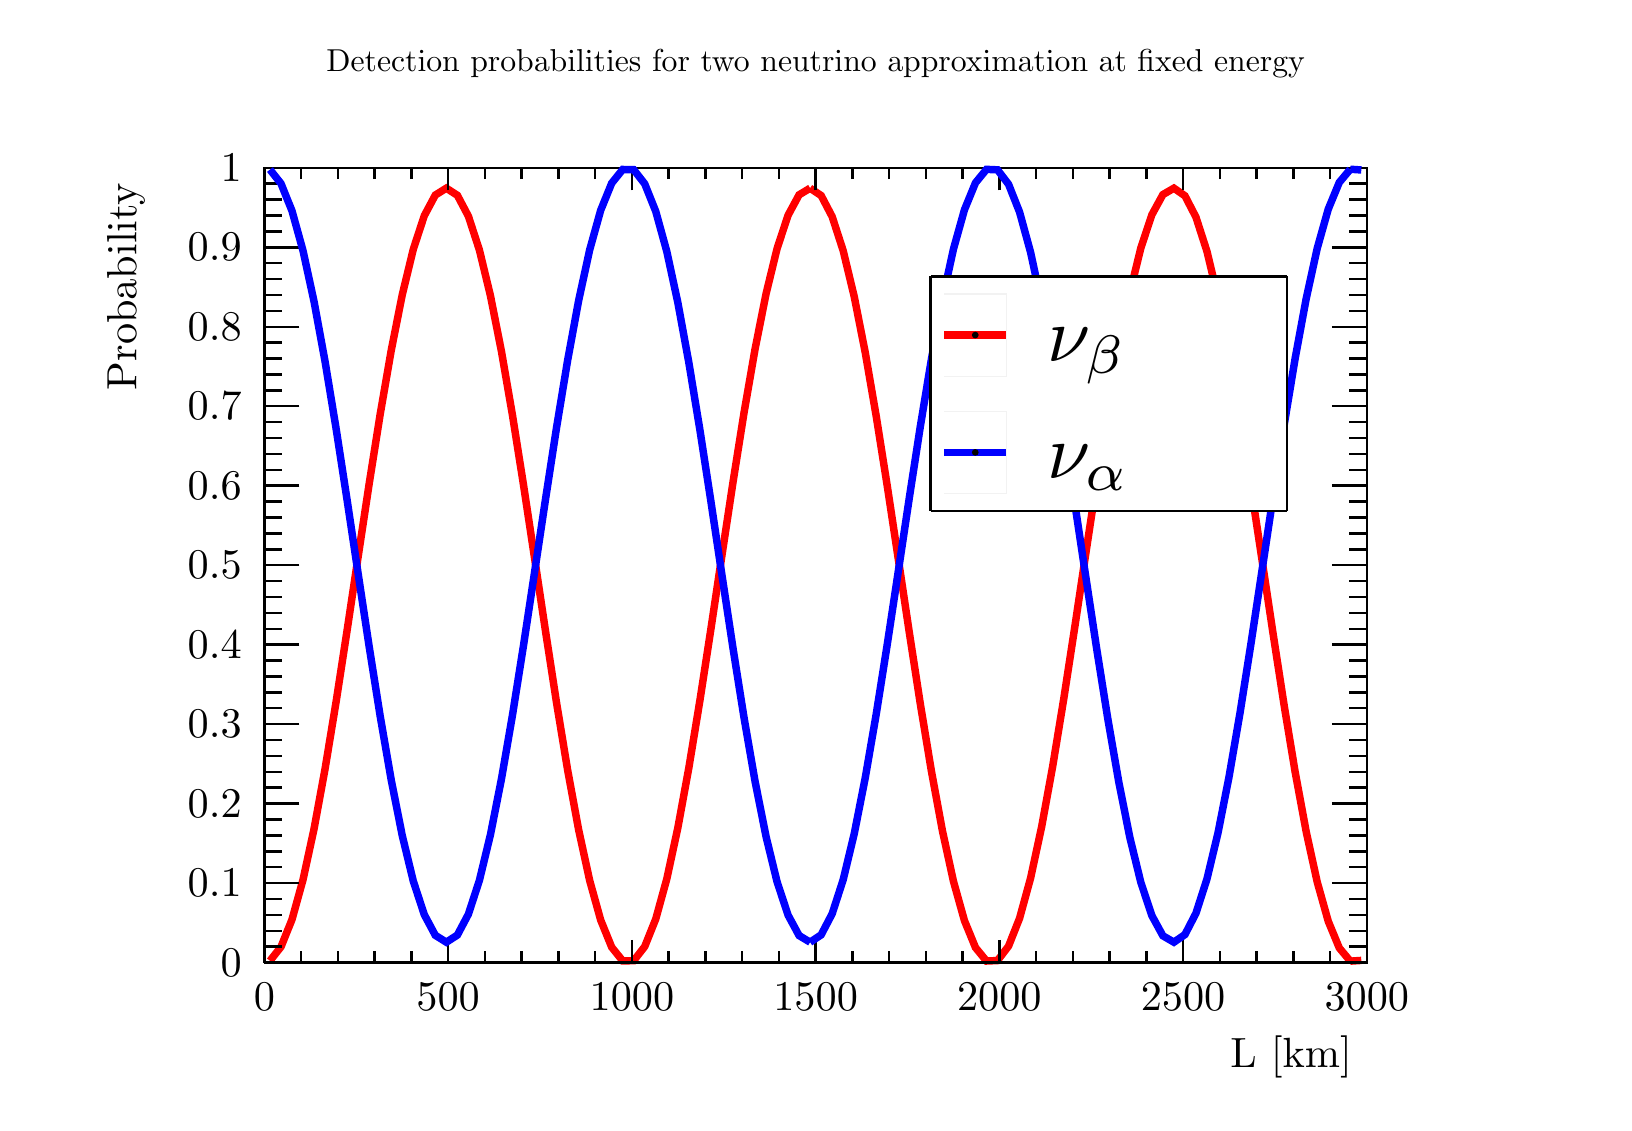
\begin{tikzpicture}
\pgfdeclareplotmark{cross} {
\pgfpathmoveto{\pgfpoint{-0.3\pgfplotmarksize}{\pgfplotmarksize}}
\pgfpathlineto{\pgfpoint{+0.3\pgfplotmarksize}{\pgfplotmarksize}}
\pgfpathlineto{\pgfpoint{+0.3\pgfplotmarksize}{0.3\pgfplotmarksize}}
\pgfpathlineto{\pgfpoint{+1\pgfplotmarksize}{0.3\pgfplotmarksize}}
\pgfpathlineto{\pgfpoint{+1\pgfplotmarksize}{-0.3\pgfplotmarksize}}
\pgfpathlineto{\pgfpoint{+0.3\pgfplotmarksize}{-0.3\pgfplotmarksize}}
\pgfpathlineto{\pgfpoint{+0.3\pgfplotmarksize}{-1.\pgfplotmarksize}}
\pgfpathlineto{\pgfpoint{-0.3\pgfplotmarksize}{-1.\pgfplotmarksize}}
\pgfpathlineto{\pgfpoint{-0.3\pgfplotmarksize}{-0.3\pgfplotmarksize}}
\pgfpathlineto{\pgfpoint{-1.\pgfplotmarksize}{-0.3\pgfplotmarksize}}
\pgfpathlineto{\pgfpoint{-1.\pgfplotmarksize}{0.3\pgfplotmarksize}}
\pgfpathlineto{\pgfpoint{-0.3\pgfplotmarksize}{0.3\pgfplotmarksize}}
\pgfpathclose
\pgfusepathqstroke
}
\pgfdeclareplotmark{cross*} {
\pgfpathmoveto{\pgfpoint{-0.3\pgfplotmarksize}{\pgfplotmarksize}}
\pgfpathlineto{\pgfpoint{+0.3\pgfplotmarksize}{\pgfplotmarksize}}
\pgfpathlineto{\pgfpoint{+0.3\pgfplotmarksize}{0.3\pgfplotmarksize}}
\pgfpathlineto{\pgfpoint{+1\pgfplotmarksize}{0.3\pgfplotmarksize}}
\pgfpathlineto{\pgfpoint{+1\pgfplotmarksize}{-0.3\pgfplotmarksize}}
\pgfpathlineto{\pgfpoint{+0.3\pgfplotmarksize}{-0.3\pgfplotmarksize}}
\pgfpathlineto{\pgfpoint{+0.3\pgfplotmarksize}{-1.\pgfplotmarksize}}
\pgfpathlineto{\pgfpoint{-0.3\pgfplotmarksize}{-1.\pgfplotmarksize}}
\pgfpathlineto{\pgfpoint{-0.3\pgfplotmarksize}{-0.3\pgfplotmarksize}}
\pgfpathlineto{\pgfpoint{-1.\pgfplotmarksize}{-0.3\pgfplotmarksize}}
\pgfpathlineto{\pgfpoint{-1.\pgfplotmarksize}{0.3\pgfplotmarksize}}
\pgfpathlineto{\pgfpoint{-0.3\pgfplotmarksize}{0.3\pgfplotmarksize}}
\pgfpathclose
\pgfusepathqfillstroke
}
\pgfdeclareplotmark{newstar} {
\pgfpathmoveto{\pgfqpoint{0pt}{\pgfplotmarksize}}
\pgfpathlineto{\pgfqpointpolar{44}{0.5\pgfplotmarksize}}
\pgfpathlineto{\pgfqpointpolar{18}{\pgfplotmarksize}}
\pgfpathlineto{\pgfqpointpolar{-20}{0.5\pgfplotmarksize}}
\pgfpathlineto{\pgfqpointpolar{-54}{\pgfplotmarksize}}
\pgfpathlineto{\pgfqpointpolar{-90}{0.5\pgfplotmarksize}}
\pgfpathlineto{\pgfqpointpolar{234}{\pgfplotmarksize}}
\pgfpathlineto{\pgfqpointpolar{198}{0.5\pgfplotmarksize}}
\pgfpathlineto{\pgfqpointpolar{162}{\pgfplotmarksize}}
\pgfpathlineto{\pgfqpointpolar{134}{0.5\pgfplotmarksize}}
\pgfpathclose
\pgfusepathqstroke
}
\pgfdeclareplotmark{newstar*} {
\pgfpathmoveto{\pgfqpoint{0pt}{\pgfplotmarksize}}
\pgfpathlineto{\pgfqpointpolar{44}{0.5\pgfplotmarksize}}
\pgfpathlineto{\pgfqpointpolar{18}{\pgfplotmarksize}}
\pgfpathlineto{\pgfqpointpolar{-20}{0.5\pgfplotmarksize}}
\pgfpathlineto{\pgfqpointpolar{-54}{\pgfplotmarksize}}
\pgfpathlineto{\pgfqpointpolar{-90}{0.5\pgfplotmarksize}}
\pgfpathlineto{\pgfqpointpolar{234}{\pgfplotmarksize}}
\pgfpathlineto{\pgfqpointpolar{198}{0.5\pgfplotmarksize}}
\pgfpathlineto{\pgfqpointpolar{162}{\pgfplotmarksize}}
\pgfpathlineto{\pgfqpointpolar{134}{0.5\pgfplotmarksize}}
\pgfpathclose
\pgfusepathqfillstroke
}
\definecolor{c}{rgb}{1,1,1};
\draw [color=c, fill=c] (0,0) rectangle (20,13.639);
\draw [color=c, fill=c] (3,1.77307) rectangle (17,11.8659);
\definecolor{c}{rgb}{0,0,0};
\draw [c,line width=0.9] (3,1.77307) -- (3,11.8659) -- (17,11.8659) -- (17,1.77307) -- (3,1.77307);
\definecolor{c}{rgb}{1,1,1};
\draw [color=c, fill=c] (3,1.77307) rectangle (17,11.8659);
\definecolor{c}{rgb}{0,0,0};
\draw [c,line width=0.9] (3,1.77307) -- (3,11.8659) -- (17,11.8659) -- (17,1.77307) -- (3,1.77307);
\definecolor{c}{rgb}{1,0,0};
\draw [c,line width=2.7] (3.07,1.79535) -- (3.21,1.97246) -- (3.35,2.32025) -- (3.49,2.82616) -- (3.63,3.47188) -- (3.77,4.23404) -- (3.91,5.08507) -- (4.05,5.99418) -- (4.19,6.92847) -- (4.33,7.85415) -- (4.47,8.73772) -- (4.61,9.54721) --
 (4.75,10.2533) -- (4.89,10.8306) -- (5.03,11.258) -- (5.17,11.5201) -- (5.31,11.6075) -- (5.45,11.517) -- (5.59,11.2519) -- (5.73,10.8217) -- (5.87,10.2421) -- (6.01,9.53393) -- (6.15,8.72289) -- (6.29,7.83831) -- (6.43,6.91219) -- (6.57,5.97805) --
 (6.71,5.06967) -- (6.85,4.21993) -- (6.99,3.45957) -- (7.13,2.8161) -- (7.27,2.31281) -- (7.41,1.96789) -- (7.55,1.79383) -- (7.69,1.79693) -- (7.83,1.97708) -- (7.97,2.32775) -- (8.11,2.83626) -- (8.25,3.48422) -- (8.39,4.24817) -- (8.53,5.10048)
 -- (8.67,6.01032) -- (8.81,6.94475) -- (8.95,7.86998) -- (9.09,8.75253) -- (9.23,9.56046) -- (9.37,10.2646) -- (9.51,10.8393) -- (9.65,11.264) -- (9.79,11.5232) -- (9.93,11.6075);
\draw [c,line width=2.7] (9.93,11.6075) -- (10.07,11.5139) -- (10.21,11.2458) -- (10.35,10.8129) -- (10.49,10.2308) -- (10.63,9.52062) -- (10.77,8.70804) -- (10.91,7.82245) -- (11.05,6.89591) -- (11.19,5.96192) -- (11.33,5.05429) -- (11.47,4.20585)
 -- (11.61,3.4473) -- (11.75,2.80609) -- (11.89,2.30541) -- (12.03,1.96337) -- (12.17,1.79236) -- (12.31,1.79856) -- (12.45,1.98175) -- (12.59,2.3353) -- (12.73,2.84641) -- (12.87,3.4966) -- (13.01,4.26233) -- (13.15,5.11592) -- (13.29,6.02646) --
 (13.43,6.96103) -- (13.57,7.8858) -- (13.71,8.76731) -- (13.85,9.57368) -- (13.99,10.2757) -- (14.13,10.8481) -- (14.27,11.2699) -- (14.41,11.5261) -- (14.55,11.6074) -- (14.69,11.5107) -- (14.83,11.2396) -- (14.97,10.804) -- (15.11,10.2195) --
 (15.25,9.50727) -- (15.39,8.69316) -- (15.53,7.80659) -- (15.67,6.87962) -- (15.81,5.94581) -- (15.95,5.03893) -- (16.09,4.1918) -- (16.23,3.43507) -- (16.37,2.79611) -- (16.51,2.29805) -- (16.65,1.95891) -- (16.79,1.79095);
\draw [c,line width=2.7] (16.79,1.79095) -- (16.93,1.80025);
\definecolor{c}{rgb}{0,0,0};
\draw [c,line width=0.9] (3,1.77307) -- (17,1.77307);
\draw [c,line width=0.9] (3,2.05948) -- (3,1.77307);
\draw [c,line width=0.9] (3.46667,1.91628) -- (3.46667,1.77307);
\draw [c,line width=0.9] (3.93333,1.91628) -- (3.93333,1.77307);
\draw [c,line width=0.9] (4.4,1.91628) -- (4.4,1.77307);
\draw [c,line width=0.9] (4.86667,1.91628) -- (4.86667,1.77307);
\draw [c,line width=0.9] (5.33333,2.05948) -- (5.33333,1.77307);
\draw [c,line width=0.9] (5.8,1.91628) -- (5.8,1.77307);
\draw [c,line width=0.9] (6.26667,1.91628) -- (6.26667,1.77307);
\draw [c,line width=0.9] (6.73333,1.91628) -- (6.73333,1.77307);
\draw [c,line width=0.9] (7.2,1.91628) -- (7.2,1.77307);
\draw [c,line width=0.9] (7.66667,2.05948) -- (7.66667,1.77307);
\draw [c,line width=0.9] (8.13333,1.91628) -- (8.13333,1.77307);
\draw [c,line width=0.9] (8.6,1.91628) -- (8.6,1.77307);
\draw [c,line width=0.9] (9.06667,1.91628) -- (9.06667,1.77307);
\draw [c,line width=0.9] (9.53333,1.91628) -- (9.53333,1.77307);
\draw [c,line width=0.9] (10,2.05948) -- (10,1.77307);
\draw [c,line width=0.9] (10.4667,1.91628) -- (10.4667,1.77307);
\draw [c,line width=0.9] (10.9333,1.91628) -- (10.9333,1.77307);
\draw [c,line width=0.9] (11.4,1.91628) -- (11.4,1.77307);
\draw [c,line width=0.9] (11.8667,1.91628) -- (11.8667,1.77307);
\draw [c,line width=0.9] (12.3333,2.05948) -- (12.3333,1.77307);
\draw [c,line width=0.9] (12.8,1.91628) -- (12.8,1.77307);
\draw [c,line width=0.9] (13.2667,1.91628) -- (13.2667,1.77307);
\draw [c,line width=0.9] (13.7333,1.91628) -- (13.7333,1.77307);
\draw [c,line width=0.9] (14.2,1.91628) -- (14.2,1.77307);
\draw [c,line width=0.9] (14.6667,2.05948) -- (14.6667,1.77307);
\draw [c,line width=0.9] (15.1333,1.91628) -- (15.1333,1.77307);
\draw [c,line width=0.9] (15.6,1.91628) -- (15.6,1.77307);
\draw [c,line width=0.9] (16.0667,1.91628) -- (16.0667,1.77307);
\draw [c,line width=0.9] (16.5333,1.91628) -- (16.5333,1.77307);
\draw [c,line width=0.9] (17,2.05948) -- (17,1.77307);
\draw [anchor=base] (3,1.15931) node[scale=1.52731, color=c, rotate=0]{0};
\draw [anchor=base] (5.33333,1.15931) node[scale=1.52731, color=c, rotate=0]{500};
\draw [anchor=base] (7.66667,1.15931) node[scale=1.52731, color=c, rotate=0]{1000};
\draw [anchor=base] (10,1.15931) node[scale=1.52731, color=c, rotate=0]{1500};
\draw [anchor=base] (12.3333,1.15931) node[scale=1.52731, color=c, rotate=0]{2000};
\draw [anchor=base] (14.6667,1.15931) node[scale=1.52731, color=c, rotate=0]{2500};
\draw [anchor=base] (17,1.15931) node[scale=1.52731, color=c, rotate=0]{3000};
\draw [anchor= east] (17,0.572837) node[scale=1.52731, color=c, rotate=0]{L [km]};
\draw [c,line width=0.9] (3,11.8659) -- (17,11.8659);
\draw [c,line width=0.9] (3,11.5795) -- (3,11.8659);
\draw [c,line width=0.9] (3.46667,11.7227) -- (3.46667,11.8659);
\draw [c,line width=0.9] (3.93333,11.7227) -- (3.93333,11.8659);
\draw [c,line width=0.9] (4.4,11.7227) -- (4.4,11.8659);
\draw [c,line width=0.9] (4.86667,11.7227) -- (4.86667,11.8659);
\draw [c,line width=0.9] (5.33333,11.5795) -- (5.33333,11.8659);
\draw [c,line width=0.9] (5.8,11.7227) -- (5.8,11.8659);
\draw [c,line width=0.9] (6.26667,11.7227) -- (6.26667,11.8659);
\draw [c,line width=0.9] (6.73333,11.7227) -- (6.73333,11.8659);
\draw [c,line width=0.9] (7.2,11.7227) -- (7.2,11.8659);
\draw [c,line width=0.9] (7.66667,11.5795) -- (7.66667,11.8659);
\draw [c,line width=0.9] (8.13333,11.7227) -- (8.13333,11.8659);
\draw [c,line width=0.9] (8.6,11.7227) -- (8.6,11.8659);
\draw [c,line width=0.9] (9.06667,11.7227) -- (9.06667,11.8659);
\draw [c,line width=0.9] (9.53333,11.7227) -- (9.53333,11.8659);
\draw [c,line width=0.9] (10,11.5795) -- (10,11.8659);
\draw [c,line width=0.9] (10.4667,11.7227) -- (10.4667,11.8659);
\draw [c,line width=0.9] (10.9333,11.7227) -- (10.9333,11.8659);
\draw [c,line width=0.9] (11.4,11.7227) -- (11.4,11.8659);
\draw [c,line width=0.9] (11.8667,11.7227) -- (11.8667,11.8659);
\draw [c,line width=0.9] (12.3333,11.5795) -- (12.3333,11.8659);
\draw [c,line width=0.9] (12.8,11.7227) -- (12.8,11.8659);
\draw [c,line width=0.9] (13.2667,11.7227) -- (13.2667,11.8659);
\draw [c,line width=0.9] (13.7333,11.7227) -- (13.7333,11.8659);
\draw [c,line width=0.9] (14.2,11.7227) -- (14.2,11.8659);
\draw [c,line width=0.9] (14.6667,11.5795) -- (14.6667,11.8659);
\draw [c,line width=0.9] (15.1333,11.7227) -- (15.1333,11.8659);
\draw [c,line width=0.9] (15.6,11.7227) -- (15.6,11.8659);
\draw [c,line width=0.9] (16.0667,11.7227) -- (16.0667,11.8659);
\draw [c,line width=0.9] (16.5333,11.7227) -- (16.5333,11.8659);
\draw [c,line width=0.9] (17,11.5795) -- (17,11.8659);
\draw [c,line width=0.9] (3,1.77307) -- (3,11.8659);
\draw [c,line width=0.9] (3.444,1.77307) -- (3,1.77307);
\draw [c,line width=0.9] (3.222,1.97492) -- (3,1.97492);
\draw [c,line width=0.9] (3.222,2.17678) -- (3,2.17678);
\draw [c,line width=0.9] (3.222,2.37864) -- (3,2.37864);
\draw [c,line width=0.9] (3.222,2.58049) -- (3,2.58049);
\draw [c,line width=0.9] (3.444,2.78235) -- (3,2.78235);
\draw [c,line width=0.9] (3.222,2.98421) -- (3,2.98421);
\draw [c,line width=0.9] (3.222,3.18606) -- (3,3.18606);
\draw [c,line width=0.9] (3.222,3.38792) -- (3,3.38792);
\draw [c,line width=0.9] (3.222,3.58978) -- (3,3.58978);
\draw [c,line width=0.9] (3.444,3.79163) -- (3,3.79163);
\draw [c,line width=0.9] (3.222,3.99349) -- (3,3.99349);
\draw [c,line width=0.9] (3.222,4.19535) -- (3,4.19535);
\draw [c,line width=0.9] (3.222,4.3972) -- (3,4.3972);
\draw [c,line width=0.9] (3.222,4.59906) -- (3,4.59906);
\draw [c,line width=0.9] (3.444,4.80092) -- (3,4.80092);
\draw [c,line width=0.9] (3.222,5.00277) -- (3,5.00277);
\draw [c,line width=0.9] (3.222,5.20463) -- (3,5.20463);
\draw [c,line width=0.9] (3.222,5.40649) -- (3,5.40649);
\draw [c,line width=0.9] (3.222,5.60834) -- (3,5.60834);
\draw [c,line width=0.9] (3.444,5.8102) -- (3,5.8102);
\draw [c,line width=0.9] (3.222,6.01206) -- (3,6.01206);
\draw [c,line width=0.9] (3.222,6.21391) -- (3,6.21391);
\draw [c,line width=0.9] (3.222,6.41577) -- (3,6.41577);
\draw [c,line width=0.9] (3.222,6.61763) -- (3,6.61763);
\draw [c,line width=0.9] (3.444,6.81948) -- (3,6.81948);
\draw [c,line width=0.9] (3.222,7.02134) -- (3,7.02134);
\draw [c,line width=0.9] (3.222,7.2232) -- (3,7.2232);
\draw [c,line width=0.9] (3.222,7.42505) -- (3,7.42505);
\draw [c,line width=0.9] (3.222,7.62691) -- (3,7.62691);
\draw [c,line width=0.9] (3.444,7.82877) -- (3,7.82877);
\draw [c,line width=0.9] (3.222,8.03062) -- (3,8.03062);
\draw [c,line width=0.9] (3.222,8.23248) -- (3,8.23248);
\draw [c,line width=0.9] (3.222,8.43434) -- (3,8.43434);
\draw [c,line width=0.9] (3.222,8.6362) -- (3,8.6362);
\draw [c,line width=0.9] (3.444,8.83805) -- (3,8.83805);
\draw [c,line width=0.9] (3.222,9.03991) -- (3,9.03991);
\draw [c,line width=0.9] (3.222,9.24177) -- (3,9.24177);
\draw [c,line width=0.9] (3.222,9.44362) -- (3,9.44362);
\draw [c,line width=0.9] (3.222,9.64548) -- (3,9.64548);
\draw [c,line width=0.9] (3.444,9.84733) -- (3,9.84733);
\draw [c,line width=0.9] (3.222,10.0492) -- (3,10.0492);
\draw [c,line width=0.9] (3.222,10.251) -- (3,10.251);
\draw [c,line width=0.9] (3.222,10.4529) -- (3,10.4529);
\draw [c,line width=0.9] (3.222,10.6548) -- (3,10.6548);
\draw [c,line width=0.9] (3.444,10.8566) -- (3,10.8566);
\draw [c,line width=0.9] (3.222,11.0585) -- (3,11.0585);
\draw [c,line width=0.9] (3.222,11.2603) -- (3,11.2603);
\draw [c,line width=0.9] (3.222,11.4622) -- (3,11.4622);
\draw [c,line width=0.9] (3.222,11.664) -- (3,11.664);
\draw [c,line width=0.9] (3.444,11.8659) -- (3,11.8659);
\draw [anchor= east] (2.9,1.77307) node[scale=1.52731, color=c, rotate=0]{0};
\draw [anchor= east] (2.9,2.78235) node[scale=1.52731, color=c, rotate=0]{0.1};
\draw [anchor= east] (2.9,3.79163) node[scale=1.52731, color=c, rotate=0]{0.2};
\draw [anchor= east] (2.9,4.80092) node[scale=1.52731, color=c, rotate=0]{0.3};
\draw [anchor= east] (2.9,5.8102) node[scale=1.52731, color=c, rotate=0]{0.4};
\draw [anchor= east] (2.9,6.81948) node[scale=1.52731, color=c, rotate=0]{0.5};
\draw [anchor= east] (2.9,7.82877) node[scale=1.52731, color=c, rotate=0]{0.6};
\draw [anchor= east] (2.9,8.83805) node[scale=1.52731, color=c, rotate=0]{0.7};
\draw [anchor= east] (2.9,9.84733) node[scale=1.52731, color=c, rotate=0]{0.8};
\draw [anchor= east] (2.9,10.8566) node[scale=1.52731, color=c, rotate=0]{0.9};
\draw [anchor= east] (2.9,11.8659) node[scale=1.52731, color=c, rotate=0]{1};
\draw [anchor= east] (1.24,11.8659) node[scale=1.52731, color=c, rotate=90]{Probability};
\draw [c,line width=0.9] (17,1.77307) -- (17,11.8659);
\draw [c,line width=0.9] (16.556,1.77307) -- (17,1.77307);
\draw [c,line width=0.9] (16.778,1.97492) -- (17,1.97492);
\draw [c,line width=0.9] (16.778,2.17678) -- (17,2.17678);
\draw [c,line width=0.9] (16.778,2.37864) -- (17,2.37864);
\draw [c,line width=0.9] (16.778,2.58049) -- (17,2.58049);
\draw [c,line width=0.9] (16.556,2.78235) -- (17,2.78235);
\draw [c,line width=0.9] (16.778,2.98421) -- (17,2.98421);
\draw [c,line width=0.9] (16.778,3.18606) -- (17,3.18606);
\draw [c,line width=0.9] (16.778,3.38792) -- (17,3.38792);
\draw [c,line width=0.9] (16.778,3.58978) -- (17,3.58978);
\draw [c,line width=0.9] (16.556,3.79163) -- (17,3.79163);
\draw [c,line width=0.9] (16.778,3.99349) -- (17,3.99349);
\draw [c,line width=0.9] (16.778,4.19535) -- (17,4.19535);
\draw [c,line width=0.9] (16.778,4.3972) -- (17,4.3972);
\draw [c,line width=0.9] (16.778,4.59906) -- (17,4.59906);
\draw [c,line width=0.9] (16.556,4.80092) -- (17,4.80092);
\draw [c,line width=0.9] (16.778,5.00277) -- (17,5.00277);
\draw [c,line width=0.9] (16.778,5.20463) -- (17,5.20463);
\draw [c,line width=0.9] (16.778,5.40649) -- (17,5.40649);
\draw [c,line width=0.9] (16.778,5.60834) -- (17,5.60834);
\draw [c,line width=0.9] (16.556,5.8102) -- (17,5.8102);
\draw [c,line width=0.9] (16.778,6.01206) -- (17,6.01206);
\draw [c,line width=0.9] (16.778,6.21391) -- (17,6.21391);
\draw [c,line width=0.9] (16.778,6.41577) -- (17,6.41577);
\draw [c,line width=0.9] (16.778,6.61763) -- (17,6.61763);
\draw [c,line width=0.9] (16.556,6.81948) -- (17,6.81948);
\draw [c,line width=0.9] (16.778,7.02134) -- (17,7.02134);
\draw [c,line width=0.9] (16.778,7.2232) -- (17,7.2232);
\draw [c,line width=0.9] (16.778,7.42505) -- (17,7.42505);
\draw [c,line width=0.9] (16.778,7.62691) -- (17,7.62691);
\draw [c,line width=0.9] (16.556,7.82877) -- (17,7.82877);
\draw [c,line width=0.9] (16.778,8.03062) -- (17,8.03062);
\draw [c,line width=0.9] (16.778,8.23248) -- (17,8.23248);
\draw [c,line width=0.9] (16.778,8.43434) -- (17,8.43434);
\draw [c,line width=0.9] (16.778,8.6362) -- (17,8.6362);
\draw [c,line width=0.9] (16.556,8.83805) -- (17,8.83805);
\draw [c,line width=0.9] (16.778,9.03991) -- (17,9.03991);
\draw [c,line width=0.9] (16.778,9.24177) -- (17,9.24177);
\draw [c,line width=0.9] (16.778,9.44362) -- (17,9.44362);
\draw [c,line width=0.9] (16.778,9.64548) -- (17,9.64548);
\draw [c,line width=0.9] (16.556,9.84733) -- (17,9.84733);
\draw [c,line width=0.9] (16.778,10.0492) -- (17,10.0492);
\draw [c,line width=0.9] (16.778,10.251) -- (17,10.251);
\draw [c,line width=0.9] (16.778,10.4529) -- (17,10.4529);
\draw [c,line width=0.9] (16.778,10.6548) -- (17,10.6548);
\draw [c,line width=0.9] (16.556,10.8566) -- (17,10.8566);
\draw [c,line width=0.9] (16.778,11.0585) -- (17,11.0585);
\draw [c,line width=0.9] (16.778,11.2603) -- (17,11.2603);
\draw [c,line width=0.9] (16.778,11.4622) -- (17,11.4622);
\draw [c,line width=0.9] (16.778,11.664) -- (17,11.664);
\draw [c,line width=0.9] (16.556,11.8659) -- (17,11.8659);
\definecolor{c}{rgb}{0,0,1};
\draw [c,line width=2.7] (3.07,11.8436) -- (3.21,11.6665) -- (3.35,11.3187) -- (3.49,10.8128) -- (3.63,10.1671) -- (3.77,9.40493) -- (3.91,8.5539) -- (4.05,7.64479) -- (4.19,6.7105) -- (4.33,5.78482) -- (4.47,4.90125) -- (4.61,4.09176) --
 (4.75,3.38563) -- (4.89,2.80841) -- (5.03,2.381) -- (5.17,2.11884) -- (5.31,2.03143) -- (5.45,2.12192) -- (5.59,2.38706) -- (5.73,2.81723) -- (5.87,3.39688) -- (6.01,4.10504) -- (6.15,4.91608) -- (6.29,5.80066) -- (6.43,6.72678) -- (6.57,7.66092) --
 (6.71,8.5693) -- (6.85,9.41904) -- (6.99,10.1794) -- (7.13,10.8229) -- (7.27,11.3262) -- (7.41,11.6711) -- (7.55,11.8451) -- (7.69,11.842) -- (7.83,11.6619) -- (7.97,11.3112) -- (8.11,10.8027) -- (8.25,10.1547) -- (8.39,9.3908) -- (8.53,8.53848) --
 (8.67,7.62865) -- (8.81,6.69422) -- (8.95,5.76899) -- (9.09,4.88644) -- (9.23,4.07851) -- (9.37,3.37442) -- (9.51,2.79964) -- (9.65,2.37498) -- (9.79,2.1158) -- (9.93,2.03148);
\draw [c,line width=2.7] (9.93,2.03148) -- (10.07,2.12506) -- (10.21,2.39317) -- (10.35,2.82609) -- (10.49,3.40817) -- (10.63,4.11835) -- (10.77,4.93093) -- (10.91,5.81652) -- (11.05,6.74306) -- (11.19,7.67705) -- (11.33,8.58468) -- (11.47,9.43312)
 -- (11.61,10.1917) -- (11.75,10.8329) -- (11.89,11.3336) -- (12.03,11.6756) -- (12.17,11.8466) -- (12.31,11.8404) -- (12.45,11.6572) -- (12.59,11.3037) -- (12.73,10.7926) -- (12.87,10.1424) -- (13.01,9.37664) -- (13.15,8.52305) -- (13.29,7.61251) --
 (13.43,6.67794) -- (13.57,5.75317) -- (13.71,4.87166) -- (13.85,4.06529) -- (13.99,3.36324) -- (14.13,2.79092) -- (14.27,2.36902) -- (14.41,2.11282) -- (14.55,2.03159) -- (14.69,2.12826) -- (14.83,2.39933) -- (14.97,2.835) -- (15.11,3.4195) --
 (15.25,4.1317) -- (15.39,4.94581) -- (15.53,5.83238) -- (15.67,6.75935) -- (15.81,7.69316) -- (15.95,8.60004) -- (16.09,9.44717) -- (16.23,10.2039) -- (16.37,10.8429) -- (16.51,11.3409) -- (16.65,11.6801) -- (16.79,11.848);
\draw [c,line width=2.7] (16.79,11.848) -- (16.93,11.8387);
\definecolor{c}{rgb}{1,1,1};
\draw [color=c, fill=c] (2,12.8206) rectangle (18,13.5708);
\definecolor{c}{rgb}{0,0,0};
\draw (10,13.1957) node[scale=1.14549, color=c, rotate=0]{Detection probabilities for two neutrino approximation at fixed energy};
\definecolor{c}{rgb}{1,1,1};
\draw [color=c, fill=c] (11.4613,7.50716) rectangle (15.9885,10.4871);
\definecolor{c}{rgb}{0,0,0};
\draw [c,line width=0.9] (11.4613,7.50716) -- (15.9885,7.50716);
\draw [c,line width=0.9] (15.9885,7.50716) -- (15.9885,10.4871);
\draw [c,line width=0.9] (15.9885,10.4871) -- (11.4613,10.4871);
\draw [c,line width=0.9] (11.4613,10.4871) -- (11.4613,7.50716);
\draw [anchor=base west] (12.5931,9.40688) node[scale=2.80008, color=c, rotate=0]{$\nu_{\beta}$};
\definecolor{c}{rgb}{0.95,0.95,0.95};
\draw [c] (11.6311,9.22063) -- (12.4234,9.22063) -- (12.4234,10.2636) -- (11.6311,10.2636);
\definecolor{c}{rgb}{1,0,0};
\draw [c,line width=2.7] (11.6311,9.74212) -- (12.4234,9.74212);
\definecolor{c}{rgb}{0,0,0};
\foreach \P in {(12.0272,9.74212)}{\draw[mark options={color=c,fill=c},mark size=2.402402pt,mark=*,mark size=1pt] plot coordinates {\P};}
\draw [anchor=base west] (12.5931,7.91691) node[scale=2.80008, color=c, rotate=0]{$\nu_{\alpha}$};
\definecolor{c}{rgb}{0.95,0.95,0.95};
\draw [c] (11.6311,7.73066) -- (12.4234,7.73066) -- (12.4234,8.77364) -- (11.6311,8.77364);
\definecolor{c}{rgb}{0,0,1};
\draw [c,line width=2.7] (11.6311,8.25215) -- (12.4234,8.25215);
\definecolor{c}{rgb}{0,0,0};
\foreach \P in {(12.0272,8.25215)}{\draw[mark options={color=c,fill=c},mark size=2.402402pt,mark=*,mark size=1pt] plot coordinates {\P};}
\end{tikzpicture}

    \end{adjustbox}
    \caption{Probability of detecting an initial $\nu_{\alpha}$ as a particular flavour as a function of baseline, $L$. Here, the energy of the neutrino is 1~GeV.}
  \end{subfigure}
  \hfill
  \begin{subfigure}[t]{0.49\textwidth}
    \begin{adjustbox}{max totalsize={\textwidth}, center}
      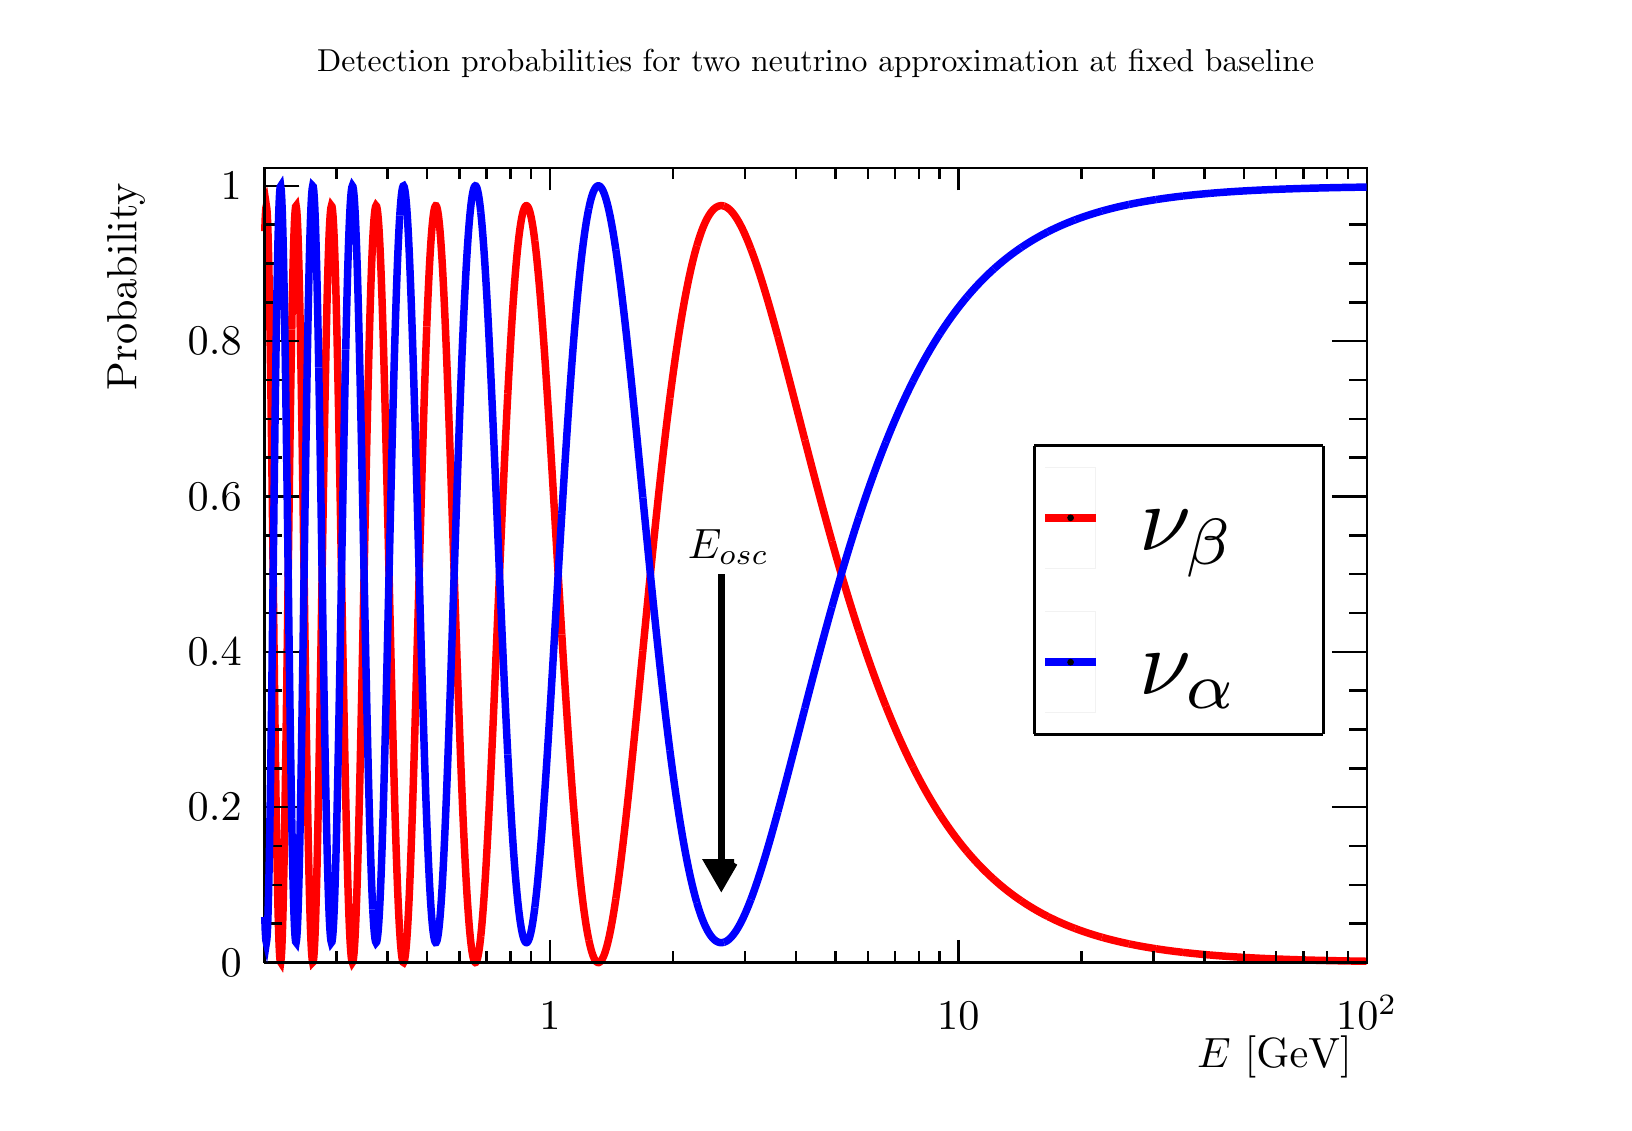
\begin{tikzpicture}
\pgfdeclareplotmark{cross} {
\pgfpathmoveto{\pgfpoint{-0.3\pgfplotmarksize}{\pgfplotmarksize}}
\pgfpathlineto{\pgfpoint{+0.3\pgfplotmarksize}{\pgfplotmarksize}}
\pgfpathlineto{\pgfpoint{+0.3\pgfplotmarksize}{0.3\pgfplotmarksize}}
\pgfpathlineto{\pgfpoint{+1\pgfplotmarksize}{0.3\pgfplotmarksize}}
\pgfpathlineto{\pgfpoint{+1\pgfplotmarksize}{-0.3\pgfplotmarksize}}
\pgfpathlineto{\pgfpoint{+0.3\pgfplotmarksize}{-0.3\pgfplotmarksize}}
\pgfpathlineto{\pgfpoint{+0.3\pgfplotmarksize}{-1.\pgfplotmarksize}}
\pgfpathlineto{\pgfpoint{-0.3\pgfplotmarksize}{-1.\pgfplotmarksize}}
\pgfpathlineto{\pgfpoint{-0.3\pgfplotmarksize}{-0.3\pgfplotmarksize}}
\pgfpathlineto{\pgfpoint{-1.\pgfplotmarksize}{-0.3\pgfplotmarksize}}
\pgfpathlineto{\pgfpoint{-1.\pgfplotmarksize}{0.3\pgfplotmarksize}}
\pgfpathlineto{\pgfpoint{-0.3\pgfplotmarksize}{0.3\pgfplotmarksize}}
\pgfpathclose
\pgfusepathqstroke
}
\pgfdeclareplotmark{cross*} {
\pgfpathmoveto{\pgfpoint{-0.3\pgfplotmarksize}{\pgfplotmarksize}}
\pgfpathlineto{\pgfpoint{+0.3\pgfplotmarksize}{\pgfplotmarksize}}
\pgfpathlineto{\pgfpoint{+0.3\pgfplotmarksize}{0.3\pgfplotmarksize}}
\pgfpathlineto{\pgfpoint{+1\pgfplotmarksize}{0.3\pgfplotmarksize}}
\pgfpathlineto{\pgfpoint{+1\pgfplotmarksize}{-0.3\pgfplotmarksize}}
\pgfpathlineto{\pgfpoint{+0.3\pgfplotmarksize}{-0.3\pgfplotmarksize}}
\pgfpathlineto{\pgfpoint{+0.3\pgfplotmarksize}{-1.\pgfplotmarksize}}
\pgfpathlineto{\pgfpoint{-0.3\pgfplotmarksize}{-1.\pgfplotmarksize}}
\pgfpathlineto{\pgfpoint{-0.3\pgfplotmarksize}{-0.3\pgfplotmarksize}}
\pgfpathlineto{\pgfpoint{-1.\pgfplotmarksize}{-0.3\pgfplotmarksize}}
\pgfpathlineto{\pgfpoint{-1.\pgfplotmarksize}{0.3\pgfplotmarksize}}
\pgfpathlineto{\pgfpoint{-0.3\pgfplotmarksize}{0.3\pgfplotmarksize}}
\pgfpathclose
\pgfusepathqfillstroke
}
\pgfdeclareplotmark{newstar} {
\pgfpathmoveto{\pgfqpoint{0pt}{\pgfplotmarksize}}
\pgfpathlineto{\pgfqpointpolar{44}{0.5\pgfplotmarksize}}
\pgfpathlineto{\pgfqpointpolar{18}{\pgfplotmarksize}}
\pgfpathlineto{\pgfqpointpolar{-20}{0.5\pgfplotmarksize}}
\pgfpathlineto{\pgfqpointpolar{-54}{\pgfplotmarksize}}
\pgfpathlineto{\pgfqpointpolar{-90}{0.5\pgfplotmarksize}}
\pgfpathlineto{\pgfqpointpolar{234}{\pgfplotmarksize}}
\pgfpathlineto{\pgfqpointpolar{198}{0.5\pgfplotmarksize}}
\pgfpathlineto{\pgfqpointpolar{162}{\pgfplotmarksize}}
\pgfpathlineto{\pgfqpointpolar{134}{0.5\pgfplotmarksize}}
\pgfpathclose
\pgfusepathqstroke
}
\pgfdeclareplotmark{newstar*} {
\pgfpathmoveto{\pgfqpoint{0pt}{\pgfplotmarksize}}
\pgfpathlineto{\pgfqpointpolar{44}{0.5\pgfplotmarksize}}
\pgfpathlineto{\pgfqpointpolar{18}{\pgfplotmarksize}}
\pgfpathlineto{\pgfqpointpolar{-20}{0.5\pgfplotmarksize}}
\pgfpathlineto{\pgfqpointpolar{-54}{\pgfplotmarksize}}
\pgfpathlineto{\pgfqpointpolar{-90}{0.5\pgfplotmarksize}}
\pgfpathlineto{\pgfqpointpolar{234}{\pgfplotmarksize}}
\pgfpathlineto{\pgfqpointpolar{198}{0.5\pgfplotmarksize}}
\pgfpathlineto{\pgfqpointpolar{162}{\pgfplotmarksize}}
\pgfpathlineto{\pgfqpointpolar{134}{0.5\pgfplotmarksize}}
\pgfpathclose
\pgfusepathqfillstroke
}
\definecolor{c}{rgb}{1,1,1};
\draw [color=c, fill=c] (0,0) rectangle (20,13.639);
\draw [color=c, fill=c] (3,1.77307) rectangle (17,11.8659);
\definecolor{c}{rgb}{0,0,0};
\draw [c,line width=0.9] (3,1.77307) -- (3,11.8659) -- (17,11.8659) -- (17,1.77307) -- (3,1.77307);
\definecolor{c}{rgb}{1,1,1};
\draw [color=c, fill=c] (3,1.77307) rectangle (17,11.8659);
\definecolor{c}{rgb}{0,0,0};
\draw [c,line width=0.9] (3,1.77307) -- (3,11.8659) -- (17,11.8659) -- (17,1.77307) -- (3,1.77307);
\definecolor{c}{rgb}{1,0,0};
\draw [c,line width=2.7] (3.0035,11.0598) -- (3.0105,11.2449) -- (3.0175,11.3537) -- (3.0245,11.385) -- (3.0315,11.339) -- (3.0385,11.2174) -- (3.0455,11.0225) -- (3.0525,10.7583) -- (3.0595,10.4295) -- (3.0665,10.0417) -- (3.0735,9.60166) --
 (3.0805,9.1165) -- (3.0875,8.5941) -- (3.0945,8.04273) -- (3.1015,7.47098) -- (3.1085,6.88764) -- (3.1155,6.30149) -- (3.1225,5.72127) -- (3.1295,5.15547) -- (3.1365,4.61223) -- (3.1435,4.09924) -- (3.1505,3.62366) -- (3.1575,3.19196) --
 (3.1645,2.80992) -- (3.1715,2.48248) -- (3.1785,2.21376) -- (3.1855,2.00699) -- (3.1925,1.86448) -- (3.1995,1.7876) -- (3.2065,1.7768) -- (3.2135,1.83162) -- (3.2205,1.95071) -- (3.2275,2.13186) -- (3.2345,2.37207) -- (3.2415,2.66759) --
 (3.2485,3.01398) -- (3.2555,3.40621) -- (3.2625,3.83872) -- (3.2695,4.30551) -- (3.2765,4.80022) -- (3.2835,5.31623) -- (3.2905,5.84676) -- (3.2975,6.38493) -- (3.3045,6.9239) -- (3.3115,7.45687) -- (3.3185,7.97729) -- (3.3255,8.4788) --
 (3.3325,8.95542) -- (3.3395,9.40155) -- (3.3465,9.81205);
\draw [c,line width=2.7] (3.3465,9.81205) -- (3.3535,10.1823) -- (3.3605,10.5082) -- (3.3675,10.7862) -- (3.3745,11.0136) -- (3.3815,11.1882) -- (3.3885,11.3083) -- (3.3955,11.373) -- (3.4025,11.3822) -- (3.4095,11.3363) -- (3.4165,11.2362) --
 (3.4235,11.0836) -- (3.4305,10.8808) -- (3.4375,10.6304) -- (3.4445,10.3357) -- (3.4515,10.0004) -- (3.4585,9.62854) -- (3.4655,9.22451) -- (3.4725,8.79302) -- (3.4795,8.33898) -- (3.4865,7.86749) -- (3.4935,7.38372) -- (3.5005,6.89293) --
 (3.5075,6.40036) -- (3.5145,5.91118) -- (3.5215,5.43046) -- (3.5285,4.96308) -- (3.5355,4.51374) -- (3.5425,4.08686) -- (3.5495,3.68656) -- (3.5565,3.31665) -- (3.5635,2.98054) -- (3.5705,2.68128) -- (3.5775,2.42149) -- (3.5845,2.20337) --
 (3.5915,2.02866) -- (3.5985,1.89865) -- (3.6055,1.8142) -- (3.6125,1.77569) -- (3.6195,1.78306) -- (3.6265,1.83582) -- (3.6335,1.93305) -- (3.6405,2.07343) -- (3.6475,2.25525) -- (3.6545,2.47644) -- (3.6615,2.7346) -- (3.6685,3.02703) --
 (3.6755,3.35077) -- (3.6825,3.70258) -- (3.6895,4.07907);
\draw [c,line width=2.7] (3.6895,4.07907) -- (3.6965,4.47663) -- (3.7035,4.89156) -- (3.7105,5.32004) -- (3.7175,5.75819) -- (3.7245,6.20211) -- (3.7315,6.64791) -- (3.7385,7.09174) -- (3.7455,7.52983) -- (3.7525,7.95852) -- (3.7595,8.37427) --
 (3.7665,8.77373) -- (3.7735,9.15371) -- (3.7805,9.51126) -- (3.7875,9.84363) -- (3.7945,10.1483) -- (3.8015,10.4232) -- (3.8085,10.6662) -- (3.8155,10.8757) -- (3.8225,11.0505) -- (3.8295,11.1893) -- (3.8365,11.2914) -- (3.8435,11.3564) --
 (3.8505,11.3842) -- (3.8575,11.3748) -- (3.8645,11.3287) -- (3.8715,11.2465) -- (3.8785,11.1292) -- (3.8855,10.9781) -- (3.8925,10.7945) -- (3.8995,10.5802) -- (3.9065,10.337) -- (3.9135,10.067) -- (3.9205,9.77235) -- (3.9275,9.45548) --
 (3.9345,9.11886) -- (3.9415,8.76511) -- (3.9485,8.39689) -- (3.9555,8.01696) -- (3.9625,7.62811) -- (3.9695,7.23313) -- (3.9765,6.83483) -- (3.9835,6.436) -- (3.9905,6.03939) -- (3.9975,5.64769) -- (4.0045,5.2635) -- (4.0115,4.88936) --
 (4.0185,4.52768) -- (4.0255,4.18074) -- (4.0325,3.85072);
\draw [c,line width=2.7] (4.0325,3.85072) -- (4.0395,3.53964) -- (4.0465,3.24934) -- (4.0535,2.98152) -- (4.0605,2.73771) -- (4.0675,2.51925) -- (4.0745,2.3273) -- (4.0815,2.16283) -- (4.0885,2.02663) -- (4.0955,1.91927) -- (4.1025,1.84117) --
 (4.1095,1.79254) -- (4.1165,1.77307) -- (4.1235,1.7836) -- (4.1305,1.8228) -- (4.1375,1.89049) -- (4.1445,1.98601) -- (4.1515,2.10854) -- (4.1585,2.25708) -- (4.1655,2.43053) -- (4.1725,2.62765) -- (4.1795,2.84706) -- (4.1865,3.08729) --
 (4.1935,3.34676) -- (4.2005,3.62383) -- (4.2075,3.91675) -- (4.2145,4.22372) -- (4.2215,4.5429) -- (4.2285,4.87239) -- (4.2355,5.21027) -- (4.2425,5.55461) -- (4.2495,5.90347) -- (4.2565,6.2549) -- (4.2635,6.60699) -- (4.2705,6.95784) --
 (4.2775,7.3056) -- (4.2845,7.64844) -- (4.2915,7.9846) -- (4.2985,8.3124) -- (4.3055,8.63019) -- (4.3125,8.93644) -- (4.3195,9.22967) -- (4.3265,9.5085) -- (4.3335,9.77166) -- (4.3405,10.018) -- (4.3475,10.2463) -- (4.3545,10.4558) --
 (4.3615,10.6455) -- (4.3685,10.8147) -- (4.3755,10.9627);
\draw [c,line width=2.7] (4.3755,10.9627) -- (4.3825,11.089) -- (4.3895,11.1933) -- (4.3965,11.2751) -- (4.4035,11.3344) -- (4.4105,11.3711) -- (4.4175,11.3851) -- (4.4245,11.3767) -- (4.4315,11.3461) -- (4.4385,11.2937) -- (4.4455,11.2198) --
 (4.4525,11.125) -- (4.4595,11.0099) -- (4.4665,10.8753) -- (4.4735,10.722) -- (4.4805,10.5507) -- (4.4875,10.3625) -- (4.4945,10.1582) -- (4.5015,9.939) -- (4.5085,9.70592) -- (4.5155,9.46012) -- (4.5225,9.20275) -- (4.5295,8.93504) --
 (4.5365,8.65821) -- (4.5435,8.37351) -- (4.5505,8.08222) -- (4.5575,7.78559) -- (4.5645,7.48491) -- (4.5715,7.18146) -- (4.5785,6.8765) -- (4.5855,6.57128) -- (4.5925,6.26704) -- (4.5995,5.96498) -- (4.6065,5.66631) -- (4.6135,5.37215) --
 (4.6205,5.08364) -- (4.6275,4.80185) -- (4.6345,4.52781) -- (4.6415,4.26251) -- (4.6485,4.00689) -- (4.6555,3.76184) -- (4.6625,3.52818) -- (4.6695,3.3067) -- (4.6765,3.0981) -- (4.6835,2.90306) -- (4.6905,2.72216) -- (4.6975,2.55594) --
 (4.7045,2.40487) -- (4.7115,2.26935) -- (4.7185,2.14975);
\draw [c,line width=2.7] (4.7185,2.14975) -- (4.7255,2.04633) -- (4.7325,1.95931) -- (4.7395,1.88886) -- (4.7465,1.83506) -- (4.7535,1.79795) -- (4.7605,1.77751) -- (4.7675,1.77307) -- (4.7745,1.78623) -- (4.7815,1.81505) -- (4.7885,1.85987) --
 (4.7955,1.92039) -- (4.8025,1.99626) -- (4.8095,2.08708) -- (4.8165,2.19241) -- (4.8235,2.31177) -- (4.8305,2.44465) -- (4.8375,2.59048) -- (4.8445,2.74867) -- (4.8515,2.9186) -- (4.8585,3.09963) -- (4.8655,3.29106) -- (4.8725,3.4922) --
 (4.8795,3.70234) -- (4.8865,3.92072) -- (4.8935,4.14661) -- (4.9005,4.37924) -- (4.9075,4.61782) -- (4.9145,4.86159) -- (4.9215,5.10976) -- (4.9285,5.36154) -- (4.9355,5.61615) -- (4.9425,5.8728) -- (4.9495,6.13073) -- (4.9565,6.38916) --
 (4.9635,6.64734) -- (4.9705,6.90452) -- (4.9775,7.15998) -- (4.9845,7.413) -- (4.9915,7.66288) -- (4.9985,7.90896) -- (5.0055,8.15056) -- (5.0125,8.38707) -- (5.0195,8.61787) -- (5.0265,8.84239) -- (5.0335,9.06006) -- (5.0405,9.27035) --
 (5.0475,9.47278) -- (5.0545,9.66686) -- (5.0615,9.85216);
\draw [c,line width=2.7] (5.0615,9.85216) -- (5.0685,10.0283) -- (5.0755,10.1948) -- (5.0825,10.3514) -- (5.0895,10.4978) -- (5.0965,10.6336) -- (5.1035,10.7587) -- (5.1105,10.8728) -- (5.1175,10.9757) -- (5.1245,11.0673) -- (5.1315,11.1474) --
 (5.1385,11.216) -- (5.1455,11.2729) -- (5.1525,11.3182) -- (5.1595,11.3519) -- (5.1665,11.3739) -- (5.1735,11.3844) -- (5.1805,11.3833) -- (5.1875,11.3709) -- (5.1945,11.3472) -- (5.2015,11.3125) -- (5.2085,11.2668) -- (5.2155,11.2105) --
 (5.2225,11.1437) -- (5.2295,11.0667) -- (5.2365,10.9797) -- (5.2435,10.8831) -- (5.2505,10.7771) -- (5.2575,10.6622) -- (5.2645,10.5385) -- (5.2715,10.4065) -- (5.2785,10.2666) -- (5.2855,10.1191) -- (5.2925,9.96439) -- (5.2995,9.80291) --
 (5.3065,9.63506) -- (5.3135,9.46126) -- (5.3205,9.28193) -- (5.3275,9.0975) -- (5.3345,8.9084) -- (5.3415,8.71507) -- (5.3485,8.51796) -- (5.3555,8.3175) -- (5.3625,8.11414) -- (5.3695,7.90831) -- (5.3765,7.70045) -- (5.3835,7.49101) --
 (5.3905,7.28042) -- (5.3975,7.0691) -- (5.4045,6.85747);
\draw [c,line width=2.7] (5.4045,6.85747) -- (5.4115,6.64596) -- (5.4185,6.43498) -- (5.4255,6.22493) -- (5.4325,6.01621) -- (5.4395,5.8092) -- (5.4465,5.60428) -- (5.4535,5.40182) -- (5.4605,5.20218) -- (5.4675,5.0057) -- (5.4745,4.81272) --
 (5.4815,4.62356) -- (5.4885,4.43854) -- (5.4955,4.25795) -- (5.5025,4.08208) -- (5.5095,3.9112) -- (5.5165,3.74557) -- (5.5235,3.58543) -- (5.5305,3.43103) -- (5.5375,3.28257) -- (5.5445,3.14026) -- (5.5515,3.00429) -- (5.5585,2.87484) --
 (5.5655,2.75206) -- (5.5725,2.63611) -- (5.5795,2.52711) -- (5.5865,2.42519) -- (5.5935,2.33045) -- (5.6005,2.24298) -- (5.6075,2.16286) -- (5.6145,2.09015) -- (5.6215,2.02491) -- (5.6285,1.96716) -- (5.6355,1.91693) -- (5.6425,1.87423) --
 (5.6495,1.83907) -- (5.6565,1.81142) -- (5.6635,1.79126) -- (5.6705,1.77855) -- (5.6775,1.77307) -- (5.6845,1.77528) -- (5.6915,1.78459) -- (5.6985,1.80109) -- (5.7055,1.82468) -- (5.7125,1.85527) -- (5.7195,1.89274) -- (5.7265,1.93698) --
 (5.7335,1.98786) -- (5.7405,2.04524) -- (5.7475,2.10898);
\draw [c,line width=2.7] (5.7475,2.10898) -- (5.7545,2.17892) -- (5.7615,2.25491) -- (5.7685,2.33678) -- (5.7755,2.42436) -- (5.7825,2.51748) -- (5.7895,2.61594) -- (5.7965,2.71957) -- (5.8035,2.82818) -- (5.8105,2.94155) -- (5.8175,3.05951) --
 (5.8245,3.18183) -- (5.8315,3.30833) -- (5.8385,3.43877) -- (5.8455,3.57297) -- (5.8525,3.71069) -- (5.8595,3.85173) -- (5.8665,3.99587) -- (5.8735,4.14289) -- (5.8805,4.29258) -- (5.8875,4.44471) -- (5.8945,4.59907) -- (5.9015,4.75545) --
 (5.9085,4.91361) -- (5.9155,5.07336) -- (5.9225,5.23446) -- (5.9295,5.39672) -- (5.9365,5.55991) -- (5.9435,5.72383) -- (5.9505,5.88828) -- (5.9575,6.05304) -- (5.9645,6.21791) -- (5.9715,6.3827) -- (5.9785,6.54721) -- (5.9855,6.71125) --
 (5.9925,6.87462) -- (5.9995,7.03715) -- (6.0065,7.19865) -- (6.0135,7.35894) -- (6.0205,7.51785) -- (6.0275,7.67522) -- (6.0345,7.83087) -- (6.0415,7.98465) -- (6.0485,8.13641) -- (6.0555,8.28598) -- (6.0625,8.43323) -- (6.0695,8.57802) --
 (6.0765,8.72021) -- (6.0835,8.85966) -- (6.0905,8.99626);
\draw [c,line width=2.7] (6.0905,8.99626) -- (6.0975,9.12988) -- (6.1045,9.26041) -- (6.1115,9.38774) -- (6.1185,9.51176) -- (6.1255,9.63237) -- (6.1325,9.74948) -- (6.1395,9.86301) -- (6.1465,9.97286) -- (6.1535,10.079) -- (6.1605,10.1812) --
 (6.1675,10.2796) -- (6.1745,10.374) -- (6.1815,10.4644) -- (6.1885,10.5508) -- (6.1955,10.633) -- (6.2025,10.7111) -- (6.2095,10.785) -- (6.2165,10.8546) -- (6.2235,10.92) -- (6.2305,10.9811) -- (6.2375,11.038) -- (6.2445,11.0905) --
 (6.2515,11.1387) -- (6.2585,11.1825) -- (6.2655,11.2221) -- (6.2725,11.2573) -- (6.2795,11.2882) -- (6.2865,11.3148) -- (6.2935,11.3371) -- (6.3005,11.3552) -- (6.3075,11.369) -- (6.3145,11.3786) -- (6.3215,11.384) -- (6.3285,11.3852) --
 (6.3355,11.3824) -- (6.3425,11.3755) -- (6.3495,11.3645) -- (6.3565,11.3495) -- (6.3635,11.3307) -- (6.3705,11.3079) -- (6.3775,11.2813) -- (6.3845,11.251) -- (6.3915,11.2169) -- (6.3985,11.1792) -- (6.4055,11.1379) -- (6.4125,11.0931) --
 (6.4195,11.0449) -- (6.4265,10.9933) -- (6.4335,10.9384);
\draw [c,line width=2.7] (6.4335,10.9384) -- (6.4405,10.8802) -- (6.4475,10.8189) -- (6.4545,10.7546) -- (6.4615,10.6872) -- (6.4685,10.6169) -- (6.4755,10.5438) -- (6.4825,10.468) -- (6.4895,10.3895) -- (6.4965,10.3084) -- (6.5035,10.2248) --
 (6.5105,10.1388) -- (6.5175,10.0505) -- (6.5245,9.95991) -- (6.5315,9.8672) -- (6.5385,9.77243) -- (6.5455,9.67568) -- (6.5525,9.57705) -- (6.5595,9.47663) -- (6.5665,9.3745) -- (6.5735,9.27075) -- (6.5805,9.16548) -- (6.5875,9.05876) --
 (6.5945,8.95068) -- (6.6015,8.84134) -- (6.6085,8.73082) -- (6.6155,8.61921) -- (6.6225,8.50659) -- (6.6295,8.39305) -- (6.6365,8.27868) -- (6.6435,8.16356) -- (6.6505,8.04776) -- (6.6575,7.93139) -- (6.6645,7.81451) -- (6.6715,7.69721) --
 (6.6785,7.57957) -- (6.6855,7.46166) -- (6.6925,7.34357) -- (6.6995,7.22538) -- (6.7065,7.10715) -- (6.7135,6.98897) -- (6.7205,6.87091) -- (6.7275,6.75303) -- (6.7345,6.63542) -- (6.7415,6.51814) -- (6.7485,6.40126) -- (6.7555,6.28484) --
 (6.7625,6.16896) -- (6.7695,6.05368) -- (6.7765,5.93906);
\draw [c,line width=2.7] (6.7765,5.93906) -- (6.7835,5.82516) -- (6.7905,5.71204) -- (6.7975,5.59977) -- (6.8045,5.4884) -- (6.8115,5.37799) -- (6.8185,5.26859) -- (6.8255,5.16025) -- (6.8325,5.05303) -- (6.8395,4.94698) -- (6.8465,4.84214) --
 (6.8535,4.73856) -- (6.8605,4.6363) -- (6.8675,4.53538) -- (6.8745,4.43587) -- (6.8815,4.33779) -- (6.8885,4.24119) -- (6.8955,4.1461) -- (6.9025,4.05257) -- (6.9095,3.96063) -- (6.9165,3.87031) -- (6.9235,3.78164) -- (6.9305,3.69466) --
 (6.9375,3.60939) -- (6.9445,3.52587) -- (6.9515,3.44412) -- (6.9585,3.36416) -- (6.9655,3.28602) -- (6.9725,3.20973) -- (6.9795,3.1353) -- (6.9865,3.06275) -- (6.9935,2.99211) -- (7.0005,2.92338) -- (7.0075,2.85659) -- (7.0145,2.79175) --
 (7.0215,2.72887) -- (7.0285,2.66796) -- (7.0355,2.60904) -- (7.0425,2.55212) -- (7.0495,2.4972) -- (7.0565,2.44429) -- (7.0635,2.3934) -- (7.0705,2.34453) -- (7.0775,2.29769) -- (7.0845,2.25288) -- (7.0915,2.21009) -- (7.0985,2.16934) --
 (7.1055,2.13061) -- (7.1125,2.09392) -- (7.1195,2.05925);
\draw [c,line width=2.7] (7.1195,2.05925) -- (7.1265,2.0266) -- (7.1335,1.99598) -- (7.1405,1.96736) -- (7.1475,1.94075) -- (7.1545,1.91615) -- (7.1615,1.89353) -- (7.1685,1.8729) -- (7.1755,1.85424) -- (7.1825,1.83754) -- (7.1895,1.8228) --
 (7.1965,1.80999) -- (7.2035,1.79912) -- (7.2105,1.79015) -- (7.2175,1.78309) -- (7.2245,1.77791) -- (7.2315,1.7746) -- (7.2385,1.77307) -- (7.2455,1.77307) -- (7.2525,1.77572) -- (7.2595,1.77973) -- (7.2665,1.78551) -- (7.2735,1.79306) --
 (7.2805,1.80236) -- (7.2875,1.81338) -- (7.2945,1.82611) -- (7.3015,1.84052) -- (7.3085,1.8566) -- (7.3155,1.87432) -- (7.3225,1.89366) -- (7.3295,1.91459) -- (7.3365,1.9371) -- (7.3435,1.96117) -- (7.3505,1.98676) -- (7.3575,2.01386) --
 (7.3645,2.04244) -- (7.3715,2.07248) -- (7.3785,2.10396) -- (7.3855,2.13684) -- (7.3925,2.17111) -- (7.3995,2.20674) -- (7.4065,2.2437) -- (7.4135,2.28197) -- (7.4205,2.32152) -- (7.4275,2.36233) -- (7.4345,2.40438) -- (7.4415,2.44763) --
 (7.4485,2.49207) -- (7.4555,2.53766) -- (7.4625,2.58438);
\draw [c,line width=2.7] (7.4625,2.58438) -- (7.4695,2.6322) -- (7.4765,2.6811) -- (7.4835,2.73105) -- (7.4905,2.78203) -- (7.4975,2.834) -- (7.5045,2.88695) -- (7.5115,2.94085) -- (7.5185,2.99567) -- (7.5255,3.05138) -- (7.5325,3.10796) --
 (7.5395,3.16539) -- (7.5465,3.22364) -- (7.5535,3.28268) -- (7.5605,3.34248) -- (7.5675,3.40303) -- (7.5745,3.46429) -- (7.5815,3.52625) -- (7.5885,3.58887) -- (7.5955,3.65213) -- (7.6025,3.71601) -- (7.6095,3.78048) -- (7.6165,3.84552) --
 (7.6235,3.9111) -- (7.6305,3.9772) -- (7.6375,4.0438) -- (7.6445,4.11086) -- (7.6515,4.17838) -- (7.6585,4.24632) -- (7.6655,4.31467) -- (7.6725,4.38339) -- (7.6795,4.45247) -- (7.6865,4.52188) -- (7.6935,4.5916) -- (7.7005,4.66162) --
 (7.7075,4.7319) -- (7.7145,4.80243) -- (7.7215,4.87318) -- (7.7285,4.94414) -- (7.7355,5.01528) -- (7.7425,5.08658) -- (7.7495,5.15803) -- (7.7565,5.2296) -- (7.7635,5.30127) -- (7.7705,5.37302) -- (7.7775,5.44484) -- (7.7845,5.51671) --
 (7.7915,5.5886) -- (7.7985,5.66049) -- (7.8055,5.73238);
\draw [c,line width=2.7] (7.8055,5.73238) -- (7.8125,5.80424) -- (7.8195,5.87606) -- (7.8265,5.94781) -- (7.8335,6.01949) -- (7.8405,6.09106) -- (7.8475,6.16253) -- (7.8545,6.23386) -- (7.8615,6.30505) -- (7.8685,6.37608) -- (7.8755,6.44693) --
 (7.8825,6.51759) -- (7.8895,6.58805) -- (7.8965,6.65828) -- (7.9035,6.72828) -- (7.9105,6.79804) -- (7.9175,6.86753) -- (7.9245,6.93674) -- (7.9315,7.00566) -- (7.9385,7.07429) -- (7.9455,7.1426) -- (7.9525,7.21058) -- (7.9595,7.27822) --
 (7.9665,7.34551) -- (7.9735,7.41245) -- (7.9805,7.479) -- (7.9875,7.54518) -- (7.9945,7.61096) -- (8.0015,7.67633) -- (8.0085,7.74129) -- (8.0155,7.80583) -- (8.0225,7.86992) -- (8.0295,7.93358) -- (8.0365,7.99678) -- (8.0435,8.05952) --
 (8.0505,8.12179) -- (8.0575,8.18358) -- (8.0645,8.24488) -- (8.0715,8.30569) -- (8.0785,8.36599) -- (8.0855,8.42579) -- (8.0925,8.48506) -- (8.0995,8.54381) -- (8.1065,8.60203) -- (8.1135,8.65972) -- (8.1205,8.71686) -- (8.1275,8.77345) --
 (8.1345,8.82948) -- (8.1415,8.88495) -- (8.1485,8.93986);
\draw [c,line width=2.7] (8.1485,8.93986) -- (8.1555,8.9942) -- (8.1625,9.04796) -- (8.1695,9.10113) -- (8.1765,9.15372) -- (8.1835,9.20573) -- (8.1905,9.25713) -- (8.1975,9.30794) -- (8.2045,9.35815) -- (8.2115,9.40776) -- (8.2185,9.45675) --
 (8.2255,9.50513) -- (8.2325,9.5529) -- (8.2395,9.60005) -- (8.2465,9.64658) -- (8.2535,9.69249) -- (8.2605,9.73778) -- (8.2675,9.78243) -- (8.2745,9.82646) -- (8.2815,9.86986) -- (8.2885,9.91263) -- (8.2955,9.95476) -- (8.3025,9.99626) --
 (8.3095,10.0371) -- (8.3165,10.0774) -- (8.3235,10.117) -- (8.3305,10.1559) -- (8.3375,10.1942) -- (8.3445,10.2319) -- (8.3515,10.2689) -- (8.3585,10.3053) -- (8.3655,10.3411) -- (8.3725,10.3762) -- (8.3795,10.4107) -- (8.3865,10.4446) --
 (8.3935,10.4778) -- (8.4005,10.5103) -- (8.4075,10.5423) -- (8.4145,10.5736) -- (8.4215,10.6043) -- (8.4285,10.6343) -- (8.4355,10.6637) -- (8.4425,10.6925) -- (8.4495,10.7206) -- (8.4565,10.7482) -- (8.4635,10.7751) -- (8.4705,10.8014) --
 (8.4775,10.827) -- (8.4845,10.852) -- (8.4915,10.8765);
\draw [c,line width=2.7] (8.4915,10.8765) -- (8.4985,10.9003) -- (8.5055,10.9235) -- (8.5125,10.9461) -- (8.5195,10.968) -- (8.5265,10.9894) -- (8.5335,11.0102) -- (8.5405,11.0304) -- (8.5475,11.0499) -- (8.5545,11.0689) -- (8.5615,11.0873) --
 (8.5685,11.1051) -- (8.5755,11.1223) -- (8.5825,11.139) -- (8.5895,11.155) -- (8.5965,11.1705) -- (8.6035,11.1854) -- (8.6105,11.1998) -- (8.6175,11.2135) -- (8.6245,11.2267) -- (8.6315,11.2394) -- (8.6385,11.2515) -- (8.6455,11.263) --
 (8.6525,11.274) -- (8.6595,11.2845) -- (8.6665,11.2944) -- (8.6735,11.3038) -- (8.6805,11.3126) -- (8.6875,11.3209) -- (8.6945,11.3287) -- (8.7015,11.336) -- (8.7085,11.3428) -- (8.7155,11.349) -- (8.7225,11.3547) -- (8.7295,11.36) --
 (8.7365,11.3647) -- (8.7435,11.3689) -- (8.7505,11.3726) -- (8.7575,11.3759) -- (8.7645,11.3786) -- (8.7715,11.3809) -- (8.7785,11.3827) -- (8.7855,11.384) -- (8.7925,11.3849) -- (8.7995,11.3853) -- (8.8065,11.3852) -- (8.8135,11.3847) --
 (8.8205,11.3837) -- (8.8275,11.3823) -- (8.8345,11.3805);
\draw [c,line width=2.7] (8.8345,11.3805) -- (8.8415,11.3782) -- (8.8485,11.3754) -- (8.8555,11.3723) -- (8.8625,11.3687) -- (8.8695,11.3647) -- (8.8765,11.3603) -- (8.8835,11.3554) -- (8.8905,11.3502) -- (8.8975,11.3445) -- (8.9045,11.3385) --
 (8.9115,11.3321) -- (8.9185,11.3252) -- (8.9255,11.318) -- (8.9325,11.3104) -- (8.9395,11.3024) -- (8.9465,11.2941) -- (8.9535,11.2854) -- (8.9605,11.2763) -- (8.9675,11.2669) -- (8.9745,11.2571) -- (8.9815,11.2469) -- (8.9885,11.2364) --
 (8.9955,11.2256) -- (9.0025,11.2144) -- (9.0095,11.2029) -- (9.0165,11.1911) -- (9.0235,11.1789) -- (9.0305,11.1664) -- (9.0375,11.1536) -- (9.0445,11.1405) -- (9.0515,11.127) -- (9.0585,11.1133) -- (9.0655,11.0993) -- (9.0725,11.0849) --
 (9.0795,11.0703) -- (9.0865,11.0554) -- (9.0935,11.0402) -- (9.1005,11.0247) -- (9.1075,11.009) -- (9.1145,10.9929) -- (9.1215,10.9766) -- (9.1285,10.9601) -- (9.1355,10.9433) -- (9.1425,10.9262) -- (9.1495,10.9089) -- (9.1565,10.8913) --
 (9.1635,10.8735) -- (9.1705,10.8554) -- (9.1775,10.8371);
\draw [c,line width=2.7] (9.1775,10.8371) -- (9.1845,10.8186) -- (9.1915,10.7998) -- (9.1985,10.7808) -- (9.2055,10.7616) -- (9.2125,10.7421) -- (9.2195,10.7225) -- (9.2265,10.7026) -- (9.2335,10.6826) -- (9.2405,10.6623) -- (9.2475,10.6418) --
 (9.2545,10.6212) -- (9.2615,10.6003) -- (9.2685,10.5793) -- (9.2755,10.558) -- (9.2825,10.5366) -- (9.2895,10.515) -- (9.2965,10.4932) -- (9.3035,10.4713) -- (9.3105,10.4492) -- (9.3175,10.4269) -- (9.3245,10.4044) -- (9.3315,10.3818) --
 (9.3385,10.3591) -- (9.3455,10.3362) -- (9.3525,10.3131) -- (9.3595,10.2899) -- (9.3665,10.2665) -- (9.3735,10.243) -- (9.3805,10.2194) -- (9.3875,10.1957) -- (9.3945,10.1718) -- (9.4015,10.1477) -- (9.4085,10.1236) -- (9.4155,10.0993) --
 (9.4225,10.0749) -- (9.4295,10.0504) -- (9.4365,10.0258) -- (9.4435,10.0011) -- (9.4505,9.97626) -- (9.4575,9.95132) -- (9.4645,9.92628) -- (9.4715,9.90114) -- (9.4785,9.8759) -- (9.4855,9.85057) -- (9.4925,9.82515) -- (9.4995,9.79964) --
 (9.5065,9.77404) -- (9.5135,9.74836) -- (9.5205,9.7226);
\draw [c,line width=2.7] (9.5205,9.7226) -- (9.5275,9.69676) -- (9.5345,9.67085) -- (9.5415,9.64487) -- (9.5485,9.61881) -- (9.5555,9.59268) -- (9.5625,9.56649) -- (9.5695,9.54024) -- (9.5765,9.51392) -- (9.5835,9.48755) -- (9.5905,9.46111) --
 (9.5975,9.43463) -- (9.6045,9.40809) -- (9.6115,9.38151) -- (9.6185,9.35487) -- (9.6255,9.32819) -- (9.6325,9.30147) -- (9.6395,9.27471) -- (9.6465,9.2479) -- (9.6535,9.22106) -- (9.6605,9.19419) -- (9.6675,9.16728) -- (9.6745,9.14035) --
 (9.6815,9.11338) -- (9.6885,9.08639) -- (9.6955,9.05937) -- (9.7025,9.03233) -- (9.7095,9.00527) -- (9.7165,8.97818) -- (9.7235,8.95109) -- (9.7305,8.92397) -- (9.7375,8.89684) -- (9.7445,8.8697) -- (9.7515,8.84256) -- (9.7585,8.8154) --
 (9.7655,8.78823) -- (9.7725,8.76106) -- (9.7795,8.73389) -- (9.7865,8.70671) -- (9.7935,8.67954) -- (9.8005,8.65236) -- (9.8075,8.62519) -- (9.8145,8.59803) -- (9.8215,8.57086) -- (9.8285,8.54371) -- (9.8355,8.51657) -- (9.8425,8.48944) --
 (9.8495,8.46231) -- (9.8565,8.43521) -- (9.8635,8.40811);
\draw [c,line width=2.7] (9.8635,8.40811) -- (9.8705,8.38104) -- (9.8775,8.35398) -- (9.8845,8.32694) -- (9.8915,8.29992) -- (9.8985,8.27292) -- (9.9055,8.24595) -- (9.9125,8.219) -- (9.9195,8.19207) -- (9.9265,8.16517) -- (9.9335,8.1383) --
 (9.9405,8.11146) -- (9.9475,8.08464) -- (9.9545,8.05786) -- (9.9615,8.03112) -- (9.9685,8.0044) -- (9.9755,7.97772) -- (9.9825,7.95108) -- (9.9895,7.92447) -- (9.9965,7.8979) -- (10.0035,7.87137) -- (10.0105,7.84488) -- (10.0175,7.81843) --
 (10.0245,7.79203) -- (10.0315,7.76566) -- (10.0385,7.73934) -- (10.0455,7.71307) -- (10.0525,7.68684) -- (10.0595,7.66065) -- (10.0665,7.63452) -- (10.0735,7.60843) -- (10.0805,7.58239) -- (10.0875,7.55641) -- (10.0945,7.53047) -- (10.1015,7.50458)
 -- (10.1085,7.47875) -- (10.1155,7.45297) -- (10.1225,7.42725) -- (10.1295,7.40158) -- (10.1365,7.37596) -- (10.1435,7.3504) -- (10.1505,7.3249) -- (10.1575,7.29946) -- (10.1645,7.27407) -- (10.1715,7.24875) -- (10.1785,7.22348) -- (10.1855,7.19827)
 -- (10.1925,7.17313) -- (10.1995,7.14805) -- (10.2065,7.12302);
\draw [c,line width=2.7] (10.2065,7.12302) -- (10.2135,7.09806) -- (10.2205,7.07317) -- (10.2275,7.04834) -- (10.2345,7.02357) -- (10.2415,6.99887) -- (10.2485,6.97423) -- (10.2555,6.94966) -- (10.2625,6.92516) -- (10.2695,6.90072) --
 (10.2765,6.87635) -- (10.2835,6.85205) -- (10.2905,6.82781) -- (10.2975,6.80365) -- (10.3045,6.77955) -- (10.3115,6.75553) -- (10.3185,6.73157) -- (10.3255,6.70769) -- (10.3325,6.68388) -- (10.3395,6.66013) -- (10.3465,6.63646) -- (10.3535,6.61286)
 -- (10.3605,6.58934) -- (10.3675,6.56589) -- (10.3745,6.5425) -- (10.3815,6.5192) -- (10.3885,6.49596) -- (10.3955,6.47281) -- (10.4025,6.44972) -- (10.4095,6.42671) -- (10.4165,6.40377) -- (10.4235,6.38091) -- (10.4305,6.35813) -- (10.4375,6.33542)
 -- (10.4445,6.31279) -- (10.4515,6.29023) -- (10.4585,6.26775) -- (10.4655,6.24534) -- (10.4725,6.22302) -- (10.4795,6.20077) -- (10.4865,6.17859) -- (10.4935,6.1565) -- (10.5005,6.13448) -- (10.5075,6.11254) -- (10.5145,6.09067) --
 (10.5215,6.06889) -- (10.5285,6.04718) -- (10.5355,6.02555) -- (10.5425,6.004) -- (10.5495,5.98253);
\draw [c,line width=2.7] (10.5495,5.98253) -- (10.5565,5.96114) -- (10.5635,5.93982) -- (10.5705,5.91859) -- (10.5775,5.89743) -- (10.5845,5.87635) -- (10.5915,5.85535) -- (10.5985,5.83443) -- (10.6055,5.81359) -- (10.6125,5.79283) --
 (10.6195,5.77215) -- (10.6265,5.75155) -- (10.6335,5.73103) -- (10.6405,5.71059) -- (10.6475,5.69022) -- (10.6545,5.66994) -- (10.6615,5.64974) -- (10.6685,5.62961) -- (10.6755,5.60957) -- (10.6825,5.5896) -- (10.6895,5.56972) -- (10.6965,5.54991)
 -- (10.7035,5.53019) -- (10.7105,5.51054) -- (10.7175,5.49097) -- (10.7245,5.47149) -- (10.7315,5.45208) -- (10.7385,5.43275) -- (10.7455,5.4135) -- (10.7525,5.39433) -- (10.7595,5.37524) -- (10.7665,5.35623) -- (10.7735,5.3373) -- (10.7805,5.31845)
 -- (10.7875,5.29968) -- (10.7945,5.28099) -- (10.8015,5.26237) -- (10.8085,5.24384) -- (10.8155,5.22538) -- (10.8225,5.207) -- (10.8295,5.1887) -- (10.8365,5.17049) -- (10.8435,5.15234) -- (10.8505,5.13428) -- (10.8575,5.1163) -- (10.8645,5.09839)
 -- (10.8715,5.08056) -- (10.8785,5.06281) -- (10.8855,5.04514) -- (10.8925,5.02754);
\draw [c,line width=2.7] (10.8925,5.02754) -- (10.8995,5.01003) -- (10.9065,4.99259) -- (10.9135,4.97523) -- (10.9205,4.95794) -- (10.9275,4.94073) -- (10.9345,4.9236) -- (10.9415,4.90655) -- (10.9485,4.88957) -- (10.9555,4.87267) --
 (10.9625,4.85585) -- (10.9695,4.8391) -- (10.9765,4.82243) -- (10.9835,4.80583) -- (10.9905,4.78931) -- (10.9975,4.77287) -- (11.0045,4.7565) -- (11.0115,4.74021) -- (11.0185,4.72399) -- (11.0255,4.70785) -- (11.0325,4.69178) -- (11.0395,4.67578) --
 (11.0465,4.65986) -- (11.0535,4.64402) -- (11.0605,4.62825) -- (11.0675,4.61255) -- (11.0745,4.59693) -- (11.0815,4.58138) -- (11.0885,4.5659) -- (11.0955,4.5505) -- (11.1025,4.53517) -- (11.1095,4.51991) -- (11.1165,4.50473) -- (11.1235,4.48962) --
 (11.1305,4.47458) -- (11.1375,4.45961) -- (11.1445,4.44471) -- (11.1515,4.42989) -- (11.1585,4.41513) -- (11.1655,4.40045) -- (11.1725,4.38584) -- (11.1795,4.3713) -- (11.1865,4.35683) -- (11.1935,4.34243) -- (11.2005,4.3281) -- (11.2075,4.31384) --
 (11.2145,4.29965) -- (11.2215,4.28553) -- (11.2285,4.27148) -- (11.2355,4.2575);
\draw [c,line width=2.7] (11.2355,4.2575) -- (11.2425,4.24359) -- (11.2495,4.22974) -- (11.2565,4.21597) -- (11.2635,4.20226) -- (11.2705,4.18862) -- (11.2775,4.17505) -- (11.2845,4.16154) -- (11.2915,4.1481) -- (11.2985,4.13473) -- (11.3055,4.12143)
 -- (11.3125,4.10819) -- (11.3195,4.09502) -- (11.3265,4.08192) -- (11.3335,4.06888) -- (11.3405,4.05591) -- (11.3475,4.043) -- (11.3545,4.03016) -- (11.3615,4.01738) -- (11.3685,4.00467) -- (11.3755,3.99202) -- (11.3825,3.97944) -- (11.3895,3.96692)
 -- (11.3965,3.95446) -- (11.4035,3.94207) -- (11.4105,3.92974) -- (11.4175,3.91748) -- (11.4245,3.90527) -- (11.4315,3.89313) -- (11.4385,3.88106) -- (11.4455,3.86904) -- (11.4525,3.85709) -- (11.4595,3.8452) -- (11.4665,3.83337) -- (11.4735,3.8216)
 -- (11.4805,3.80989) -- (11.4875,3.79824) -- (11.4945,3.78666) -- (11.5015,3.77513) -- (11.5085,3.76366) -- (11.5155,3.75226) -- (11.5225,3.74091) -- (11.5295,3.72962) -- (11.5365,3.71839) -- (11.5435,3.70722) -- (11.5505,3.69611) --
 (11.5575,3.68506) -- (11.5645,3.67407) -- (11.5715,3.66313) -- (11.5785,3.65225);
\draw [c,line width=2.7] (11.5785,3.65225) -- (11.5855,3.64143) -- (11.5925,3.63066) -- (11.5995,3.61996) -- (11.6065,3.60931) -- (11.6135,3.59871) -- (11.6205,3.58817) -- (11.6275,3.57769) -- (11.6345,3.56727) -- (11.6415,3.5569) --
 (11.6485,3.54658) -- (11.6555,3.53632) -- (11.6625,3.52611) -- (11.6695,3.51596) -- (11.6765,3.50587) -- (11.6835,3.49582) -- (11.6905,3.48584) -- (11.6975,3.4759) -- (11.7045,3.46602) -- (11.7115,3.45619) -- (11.7185,3.44642) -- (11.7255,3.43669)
 -- (11.7325,3.42702) -- (11.7395,3.4174) -- (11.7465,3.40784) -- (11.7535,3.39832) -- (11.7605,3.38886) -- (11.7675,3.37945) -- (11.7745,3.37009) -- (11.7815,3.36078) -- (11.7885,3.35152) -- (11.7955,3.34231) -- (11.8025,3.33316) --
 (11.8095,3.32405) -- (11.8165,3.31499) -- (11.8235,3.30598) -- (11.8305,3.29702) -- (11.8375,3.28811) -- (11.8445,3.27925) -- (11.8515,3.27043) -- (11.8585,3.26167) -- (11.8655,3.25295) -- (11.8725,3.24428) -- (11.8795,3.23566) -- (11.8865,3.22709)
 -- (11.8935,3.21856) -- (11.9005,3.21008) -- (11.9075,3.20165) -- (11.9145,3.19326) -- (11.9215,3.18492);
\draw [c,line width=2.7] (11.9215,3.18492) -- (11.9285,3.17663) -- (11.9355,3.16838) -- (11.9425,3.16018) -- (11.9495,3.15202) -- (11.9565,3.14391) -- (11.9635,3.13584) -- (11.9705,3.12782) -- (11.9775,3.11984) -- (11.9845,3.11191) --
 (11.9915,3.10402) -- (11.9985,3.09618) -- (12.0055,3.08838) -- (12.0125,3.08062) -- (12.0195,3.0729) -- (12.0265,3.06523) -- (12.0335,3.05761) -- (12.0405,3.05002) -- (12.0475,3.04248) -- (12.0545,3.03498) -- (12.0615,3.02752) -- (12.0685,3.0201) --
 (12.0755,3.01273) -- (12.0825,3.00539) -- (12.0895,2.9981) -- (12.0965,2.99085) -- (12.1035,2.98364) -- (12.1105,2.97647) -- (12.1175,2.96934) -- (12.1245,2.96225) -- (12.1315,2.9552) -- (12.1385,2.94819) -- (12.1455,2.94122) -- (12.1525,2.93429) --
 (12.1595,2.9274) -- (12.1665,2.92055) -- (12.1735,2.91373) -- (12.1805,2.90696) -- (12.1875,2.90022) -- (12.1945,2.89352) -- (12.2015,2.88686) -- (12.2085,2.88024) -- (12.2155,2.87366) -- (12.2225,2.86711) -- (12.2295,2.8606) -- (12.2365,2.85413) --
 (12.2435,2.84769) -- (12.2505,2.84129) -- (12.2575,2.83493) -- (12.2645,2.8286);
\draw [c,line width=2.7] (12.2645,2.8286) -- (12.2715,2.82231) -- (12.2785,2.81606) -- (12.2855,2.80984) -- (12.2925,2.80366) -- (12.2995,2.79751) -- (12.3065,2.79139) -- (12.3135,2.78532) -- (12.3205,2.77927) -- (12.3275,2.77327) --
 (12.3345,2.76729) -- (12.3415,2.76135) -- (12.3485,2.75545) -- (12.3555,2.74958) -- (12.3625,2.74374) -- (12.3695,2.73794) -- (12.3765,2.73217) -- (12.3835,2.72643) -- (12.3905,2.72072) -- (12.3975,2.71505) -- (12.4045,2.70941) -- (12.4115,2.70381)
 -- (12.4185,2.69824) -- (12.4255,2.69269) -- (12.4325,2.68718) -- (12.4395,2.68171) -- (12.4465,2.67626) -- (12.4535,2.67085) -- (12.4605,2.66546) -- (12.4675,2.66011) -- (12.4745,2.65479) -- (12.4815,2.6495) -- (12.4885,2.64424) --
 (12.4955,2.63901) -- (12.5025,2.63381) -- (12.5095,2.62864) -- (12.5165,2.62351) -- (12.5235,2.6184) -- (12.5305,2.61332) -- (12.5375,2.60827) -- (12.5445,2.60325) -- (12.5515,2.59826) -- (12.5585,2.5933) -- (12.5655,2.58836) -- (12.5725,2.58346) --
 (12.5795,2.57858) -- (12.5865,2.57374) -- (12.5935,2.56892) -- (12.6005,2.56413) -- (12.6075,2.55937);
\draw [c,line width=2.7] (12.6075,2.55937) -- (12.6145,2.55463) -- (12.6215,2.54992) -- (12.6285,2.54524) -- (12.6355,2.54059) -- (12.6425,2.53597) -- (12.6495,2.53137) -- (12.6565,2.5268) -- (12.6635,2.52225) -- (12.6705,2.51774) --
 (12.6775,2.51324) -- (12.6845,2.50878) -- (12.6915,2.50434) -- (12.6985,2.49993) -- (12.7055,2.49554) -- (12.7125,2.49118) -- (12.7195,2.48684) -- (12.7265,2.48253) -- (12.7335,2.47825) -- (12.7405,2.47399) -- (12.7475,2.46976) -- (12.7545,2.46555)
 -- (12.7615,2.46136) -- (12.7685,2.4572) -- (12.7755,2.45307) -- (12.7825,2.44896) -- (12.7895,2.44487) -- (12.7965,2.44081) -- (12.8035,2.43677) -- (12.8105,2.43275) -- (12.8175,2.42876) -- (12.8245,2.42479) -- (12.8315,2.42085) --
 (12.8385,2.41693) -- (12.8455,2.41303) -- (12.8525,2.40915) -- (12.8595,2.4053) -- (12.8665,2.40147) -- (12.8735,2.39767) -- (12.8805,2.39388) -- (12.8875,2.39012) -- (12.8945,2.38638) -- (12.9015,2.38266) -- (12.9085,2.37897) -- (12.9155,2.37529)
 -- (12.9225,2.37164) -- (12.9295,2.36801) -- (12.9365,2.36441) -- (12.9435,2.36082) -- (12.9505,2.35725);
\draw [c,line width=2.7] (12.9505,2.35725) -- (12.9575,2.35371) -- (12.9645,2.35018) -- (12.9715,2.34668) -- (12.9785,2.3432) -- (12.9855,2.33974) -- (12.9925,2.3363) -- (12.9995,2.33288) -- (13.0065,2.32948) -- (13.0135,2.3261) -- (13.0205,2.32274)
 -- (13.0275,2.3194) -- (13.0345,2.31608) -- (13.0415,2.31278) -- (13.0485,2.3095) -- (13.0555,2.30624) -- (13.0625,2.303) -- (13.0695,2.29978) -- (13.0765,2.29658) -- (13.0835,2.29339) -- (13.0905,2.29023) -- (13.0975,2.28708) -- (13.1045,2.28395)
 -- (13.1115,2.28085) -- (13.1185,2.27776) -- (13.1255,2.27469) -- (13.1325,2.27163) -- (13.1395,2.2686) -- (13.1465,2.26558) -- (13.1535,2.26258) -- (13.1605,2.2596) -- (13.1675,2.25664) -- (13.1745,2.2537) -- (13.1815,2.25077) -- (13.1885,2.24786)
 -- (13.1955,2.24497) -- (13.2025,2.24209) -- (13.2095,2.23923) -- (13.2165,2.23639) -- (13.2235,2.23357) -- (13.2305,2.23076) -- (13.2375,2.22797) -- (13.2445,2.2252) -- (13.2515,2.22244) -- (13.2585,2.2197) -- (13.2655,2.21698) -- (13.2725,2.21427)
 -- (13.2795,2.21158) -- (13.2865,2.2089) -- (13.2935,2.20625);
\draw [c,line width=2.7] (13.2935,2.20625) -- (13.3005,2.2036) -- (13.3075,2.20098) -- (13.3145,2.19836) -- (13.3215,2.19577) -- (13.3285,2.19319) -- (13.3355,2.19062) -- (13.3425,2.18808) -- (13.3495,2.18554) -- (13.3565,2.18302) --
 (13.3635,2.18052) -- (13.3705,2.17803) -- (13.3775,2.17556) -- (13.3845,2.1731) -- (13.3915,2.17066) -- (13.3985,2.16823) -- (13.4055,2.16581) -- (13.4125,2.16341) -- (13.4195,2.16103) -- (13.4265,2.15866) -- (13.4335,2.1563) -- (13.4405,2.15396) --
 (13.4475,2.15163) -- (13.4545,2.14932) -- (13.4615,2.14702) -- (13.4685,2.14473) -- (13.4755,2.14246) -- (13.4825,2.1402) -- (13.4895,2.13795) -- (13.4965,2.13572) -- (13.5035,2.1335) -- (13.5105,2.1313) -- (13.5175,2.12911) -- (13.5245,2.12693) --
 (13.5315,2.12476) -- (13.5385,2.12261) -- (13.5455,2.12047) -- (13.5525,2.11835) -- (13.5595,2.11623) -- (13.5665,2.11413) -- (13.5735,2.11204) -- (13.5805,2.10997) -- (13.5875,2.10791) -- (13.5945,2.10586) -- (13.6015,2.10382) -- (13.6085,2.10179)
 -- (13.6155,2.09978) -- (13.6225,2.09778) -- (13.6295,2.09579) -- (13.6365,2.09381);
\draw [c,line width=2.7] (13.6365,2.09381) -- (13.6435,2.09185) -- (13.6505,2.0899) -- (13.6575,2.08795) -- (13.6645,2.08602) -- (13.6715,2.08411) -- (13.6785,2.0822) -- (13.6855,2.08031) -- (13.6925,2.07842) -- (13.6995,2.07655) -- (13.7065,2.07469)
 -- (13.7135,2.07284) -- (13.7205,2.071) -- (13.7275,2.06918) -- (13.7345,2.06736) -- (13.7415,2.06556) -- (13.7485,2.06376) -- (13.7555,2.06198) -- (13.7625,2.06021) -- (13.7695,2.05845) -- (13.7765,2.0567) -- (13.7835,2.05496) -- (13.7905,2.05323)
 -- (13.7975,2.05151) -- (13.8045,2.0498) -- (13.8115,2.0481) -- (13.8185,2.04642) -- (13.8255,2.04474) -- (13.8325,2.04307) -- (13.8395,2.04141) -- (13.8465,2.03977) -- (13.8535,2.03813) -- (13.8605,2.0365) -- (13.8675,2.03489) -- (13.8745,2.03328)
 -- (13.8815,2.03168) -- (13.8885,2.03009) -- (13.8955,2.02852) -- (13.9025,2.02695) -- (13.9095,2.02539) -- (13.9165,2.02384) -- (13.9235,2.0223) -- (13.9305,2.02077) -- (13.9375,2.01925) -- (13.9445,2.01774) -- (13.9515,2.01623) --
 (13.9585,2.01474) -- (13.9655,2.01325) -- (13.9725,2.01178) -- (13.9795,2.01031);
\draw [c,line width=2.7] (13.9795,2.01031) -- (13.9865,2.00885) -- (13.9935,2.00741) -- (14.0005,2.00596) -- (14.0075,2.00453) -- (14.0145,2.00311) -- (14.0215,2.0017) -- (14.0285,2.00029) -- (14.0355,1.9989) -- (14.0425,1.99751) -- (14.0495,1.99613)
 -- (14.0565,1.99476) -- (14.0635,1.99339) -- (14.0705,1.99204) -- (14.0775,1.99069) -- (14.0845,1.98935) -- (14.0915,1.98803) -- (14.0985,1.9867) -- (14.1055,1.98539) -- (14.1125,1.98408) -- (14.1195,1.98279) -- (14.1265,1.9815) -- (14.1335,1.98021)
 -- (14.1405,1.97894) -- (14.1475,1.97767) -- (14.1545,1.97642) -- (14.1615,1.97516) -- (14.1685,1.97392) -- (14.1755,1.97269) -- (14.1825,1.97146) -- (14.1895,1.97024) -- (14.1965,1.96902) -- (14.2035,1.96782) -- (14.2105,1.96662) --
 (14.2175,1.96543) -- (14.2245,1.96424) -- (14.2315,1.96307) -- (14.2385,1.9619) -- (14.2455,1.96074) -- (14.2525,1.95958) -- (14.2595,1.95843) -- (14.2665,1.95729) -- (14.2735,1.95616) -- (14.2805,1.95503) -- (14.2875,1.95391) -- (14.2945,1.9528) --
 (14.3015,1.95169) -- (14.3085,1.95059) -- (14.3155,1.9495) -- (14.3225,1.94841);
\draw [c,line width=2.7] (14.3225,1.94841) -- (14.3295,1.94733) -- (14.3365,1.94626) -- (14.3435,1.94519) -- (14.3505,1.94413) -- (14.3575,1.94308) -- (14.3645,1.94203) -- (14.3715,1.94099) -- (14.3785,1.93996) -- (14.3855,1.93893) --
 (14.3925,1.93791) -- (14.3995,1.93689) -- (14.4065,1.93588) -- (14.4135,1.93488) -- (14.4205,1.93388) -- (14.4275,1.93289) -- (14.4345,1.93191) -- (14.4415,1.93093) -- (14.4485,1.92996) -- (14.4555,1.92899) -- (14.4625,1.92803) -- (14.4695,1.92707)
 -- (14.4765,1.92612) -- (14.4835,1.92518) -- (14.4905,1.92424) -- (14.4975,1.92331) -- (14.5045,1.92239) -- (14.5115,1.92147) -- (14.5185,1.92055) -- (14.5255,1.91964) -- (14.5325,1.91874) -- (14.5395,1.91784) -- (14.5465,1.91695) --
 (14.5535,1.91606) -- (14.5605,1.91518) -- (14.5675,1.9143) -- (14.5745,1.91343) -- (14.5815,1.91257) -- (14.5885,1.91171) -- (14.5955,1.91085) -- (14.6025,1.91) -- (14.6095,1.90916) -- (14.6165,1.90832) -- (14.6235,1.90749) -- (14.6305,1.90666) --
 (14.6375,1.90583) -- (14.6445,1.90501) -- (14.6515,1.9042) -- (14.6585,1.90339) -- (14.6655,1.90259);
\draw [c,line width=2.7] (14.6655,1.90259) -- (14.6725,1.90179) -- (14.6795,1.901) -- (14.6865,1.90021) -- (14.6935,1.89942) -- (14.7005,1.89864) -- (14.7075,1.89787) -- (14.7145,1.8971) -- (14.7215,1.89633) -- (14.7285,1.89557) -- (14.7355,1.89482)
 -- (14.7425,1.89407) -- (14.7495,1.89332) -- (14.7565,1.89258) -- (14.7635,1.89184) -- (14.7705,1.89111) -- (14.7775,1.89038) -- (14.7845,1.88966) -- (14.7915,1.88894) -- (14.7985,1.88822) -- (14.8055,1.88751) -- (14.8125,1.8868) -- (14.8195,1.8861)
 -- (14.8265,1.8854) -- (14.8335,1.88471) -- (14.8405,1.88402) -- (14.8475,1.88334) -- (14.8545,1.88266) -- (14.8615,1.88198) -- (14.8685,1.88131) -- (14.8755,1.88064) -- (14.8825,1.87998) -- (14.8895,1.87932) -- (14.8965,1.87866) --
 (14.9035,1.87801) -- (14.9105,1.87736) -- (14.9175,1.87672) -- (14.9245,1.87608) -- (14.9315,1.87544) -- (14.9385,1.87481) -- (14.9455,1.87418) -- (14.9525,1.87356) -- (14.9595,1.87294) -- (14.9665,1.87232) -- (14.9735,1.87171) -- (14.9805,1.8711)
 -- (14.9875,1.87049) -- (14.9945,1.86989) -- (15.0015,1.86929) -- (15.0085,1.8687);
\draw [c,line width=2.7] (15.0085,1.8687) -- (15.0155,1.86811) -- (15.0225,1.86752) -- (15.0295,1.86694) -- (15.0365,1.86636) -- (15.0435,1.86578) -- (15.0505,1.86521) -- (15.0575,1.86464) -- (15.0645,1.86408) -- (15.0715,1.86351) --
 (15.0785,1.86295) -- (15.0855,1.8624) -- (15.0925,1.86185) -- (15.0995,1.8613) -- (15.1065,1.86075) -- (15.1135,1.86021) -- (15.1205,1.85967) -- (15.1275,1.85914) -- (15.1345,1.85861) -- (15.1415,1.85808) -- (15.1485,1.85755) -- (15.1555,1.85703) --
 (15.1625,1.85651) -- (15.1695,1.856) -- (15.1765,1.85549) -- (15.1835,1.85498) -- (15.1905,1.85447) -- (15.1975,1.85397) -- (15.2045,1.85347) -- (15.2115,1.85297) -- (15.2185,1.85248) -- (15.2255,1.85199) -- (15.2325,1.8515) -- (15.2395,1.85102) --
 (15.2465,1.85053) -- (15.2535,1.85005) -- (15.2605,1.84958) -- (15.2675,1.84911) -- (15.2745,1.84864) -- (15.2815,1.84817) -- (15.2885,1.84771) -- (15.2955,1.84724) -- (15.3025,1.84679) -- (15.3095,1.84633) -- (15.3165,1.84588) -- (15.3235,1.84543)
 -- (15.3305,1.84498) -- (15.3375,1.84454) -- (15.3445,1.84409) -- (15.3515,1.84366);
\draw [c,line width=2.7] (15.3515,1.84366) -- (15.3585,1.84322) -- (15.3655,1.84279) -- (15.3725,1.84235) -- (15.3795,1.84193) -- (15.3865,1.8415) -- (15.3935,1.84108) -- (15.4005,1.84066) -- (15.4075,1.84024) -- (15.4145,1.83982) --
 (15.4215,1.83941) -- (15.4285,1.839) -- (15.4355,1.83859) -- (15.4425,1.83819) -- (15.4495,1.83779) -- (15.4565,1.83739) -- (15.4635,1.83699) -- (15.4705,1.83659) -- (15.4775,1.8362) -- (15.4845,1.83581) -- (15.4915,1.83542) -- (15.4985,1.83504) --
 (15.5055,1.83465) -- (15.5125,1.83427) -- (15.5195,1.8339) -- (15.5265,1.83352) -- (15.5335,1.83315) -- (15.5405,1.83277) -- (15.5475,1.8324) -- (15.5545,1.83204) -- (15.5615,1.83167) -- (15.5685,1.83131) -- (15.5755,1.83095) -- (15.5825,1.83059) --
 (15.5895,1.83024) -- (15.5965,1.82988) -- (15.6035,1.82953) -- (15.6105,1.82918) -- (15.6175,1.82884) -- (15.6245,1.82849) -- (15.6315,1.82815) -- (15.6385,1.82781) -- (15.6455,1.82747) -- (15.6525,1.82713) -- (15.6595,1.8268) -- (15.6665,1.82647)
 -- (15.6735,1.82614) -- (15.6805,1.82581) -- (15.6875,1.82548) -- (15.6945,1.82516);
\draw [c,line width=2.7] (15.6945,1.82516) -- (15.7015,1.82484) -- (15.7085,1.82452) -- (15.7155,1.8242) -- (15.7225,1.82388) -- (15.7295,1.82357) -- (15.7365,1.82325) -- (15.7435,1.82294) -- (15.7505,1.82264) -- (15.7575,1.82233) --
 (15.7645,1.82202) -- (15.7715,1.82172) -- (15.7785,1.82142) -- (15.7855,1.82112) -- (15.7925,1.82082) -- (15.7995,1.82053) -- (15.8065,1.82024) -- (15.8135,1.81994) -- (15.8205,1.81965) -- (15.8275,1.81937) -- (15.8345,1.81908) -- (15.8415,1.81879)
 -- (15.8485,1.81851) -- (15.8555,1.81823) -- (15.8625,1.81795) -- (15.8695,1.81767) -- (15.8765,1.8174) -- (15.8835,1.81712) -- (15.8905,1.81685) -- (15.8975,1.81658) -- (15.9045,1.81631) -- (15.9115,1.81604) -- (15.9185,1.81578) --
 (15.9255,1.81551) -- (15.9325,1.81525) -- (15.9395,1.81499) -- (15.9465,1.81473) -- (15.9535,1.81447) -- (15.9605,1.81422) -- (15.9675,1.81396) -- (15.9745,1.81371) -- (15.9815,1.81346) -- (15.9885,1.81321) -- (15.9955,1.81296) -- (16.0025,1.81271)
 -- (16.0095,1.81247) -- (16.0165,1.81222) -- (16.0235,1.81198) -- (16.0305,1.81174) -- (16.0375,1.8115);
\draw [c,line width=2.7] (16.0375,1.8115) -- (16.0445,1.81126) -- (16.0515,1.81103) -- (16.0585,1.81079) -- (16.0655,1.81056) -- (16.0725,1.81033) -- (16.0795,1.8101) -- (16.0865,1.80987) -- (16.0935,1.80964) -- (16.1005,1.80941) -- (16.1075,1.80919)
 -- (16.1145,1.80896) -- (16.1215,1.80874) -- (16.1285,1.80852) -- (16.1355,1.8083) -- (16.1425,1.80808) -- (16.1495,1.80787) -- (16.1565,1.80765) -- (16.1635,1.80744) -- (16.1705,1.80723) -- (16.1775,1.80701) -- (16.1845,1.8068) -- (16.1915,1.8066)
 -- (16.1985,1.80639) -- (16.2055,1.80618) -- (16.2125,1.80598) -- (16.2195,1.80577) -- (16.2265,1.80557) -- (16.2335,1.80537) -- (16.2405,1.80517) -- (16.2475,1.80497) -- (16.2545,1.80477) -- (16.2615,1.80458) -- (16.2685,1.80438) --
 (16.2755,1.80419) -- (16.2825,1.804) -- (16.2895,1.8038) -- (16.2965,1.80361) -- (16.3035,1.80342) -- (16.3105,1.80324) -- (16.3175,1.80305) -- (16.3245,1.80286) -- (16.3315,1.80268) -- (16.3385,1.8025) -- (16.3455,1.80231) -- (16.3525,1.80213) --
 (16.3595,1.80195) -- (16.3665,1.80178) -- (16.3735,1.8016) -- (16.3805,1.80142);
\draw [c,line width=2.7] (16.3805,1.80142) -- (16.3875,1.80125) -- (16.3945,1.80107) -- (16.4015,1.8009) -- (16.4085,1.80073) -- (16.4155,1.80055) -- (16.4225,1.80038) -- (16.4295,1.80021) -- (16.4365,1.80005) -- (16.4435,1.79988) --
 (16.4505,1.79971) -- (16.4575,1.79955) -- (16.4645,1.79939) -- (16.4715,1.79922) -- (16.4785,1.79906) -- (16.4855,1.7989) -- (16.4925,1.79874) -- (16.4995,1.79858) -- (16.5065,1.79842) -- (16.5135,1.79827) -- (16.5205,1.79811) -- (16.5275,1.79795)
 -- (16.5345,1.7978) -- (16.5415,1.79765) -- (16.5485,1.7975) -- (16.5555,1.79734) -- (16.5625,1.79719) -- (16.5695,1.79704) -- (16.5765,1.7969) -- (16.5835,1.79675) -- (16.5905,1.7966) -- (16.5975,1.79646) -- (16.6045,1.79631) -- (16.6115,1.79617)
 -- (16.6185,1.79602) -- (16.6255,1.79588) -- (16.6325,1.79574) -- (16.6395,1.7956) -- (16.6465,1.79546) -- (16.6535,1.79532) -- (16.6605,1.79518) -- (16.6675,1.79505) -- (16.6745,1.79491) -- (16.6815,1.79478) -- (16.6885,1.79464) --
 (16.6955,1.79451) -- (16.7025,1.79438) -- (16.7095,1.79424) -- (16.7165,1.79411) -- (16.7235,1.79398);
\draw [c,line width=2.7] (16.7235,1.79398) -- (16.7305,1.79385) -- (16.7375,1.79372) -- (16.7445,1.7936) -- (16.7515,1.79347) -- (16.7585,1.79334) -- (16.7655,1.79322) -- (16.7725,1.79309) -- (16.7795,1.79297) -- (16.7865,1.79285) --
 (16.7935,1.79272) -- (16.8005,1.7926) -- (16.8075,1.79248) -- (16.8145,1.79236) -- (16.8215,1.79224) -- (16.8285,1.79212) -- (16.8355,1.792) -- (16.8425,1.79189) -- (16.8495,1.79177) -- (16.8565,1.79165) -- (16.8635,1.79154) -- (16.8705,1.79142) --
 (16.8775,1.79131) -- (16.8845,1.7912) -- (16.8915,1.79109) -- (16.8985,1.79097) -- (16.9055,1.79086) -- (16.9125,1.79075) -- (16.9195,1.79064) -- (16.9265,1.79054) -- (16.9335,1.79043) -- (16.9405,1.79032) -- (16.9475,1.79021) -- (16.9545,1.79011)
 -- (16.9615,1.79) -- (16.9685,1.7899) -- (16.9755,1.78979) -- (16.9825,1.78969) -- (16.9895,1.78959) -- (16.9965,1.78948);
\definecolor{c}{rgb}{0,0,0};
\draw [c,line width=0.9] (3,1.77307) -- (17,1.77307);
\draw [c,line width=0.9] (3.00001,1.91628) -- (3.00001,1.77307);
\draw [c,line width=0.9] (3.91342,1.91628) -- (3.91342,1.77307);
\draw [c,line width=0.9] (4.5615,1.91628) -- (4.5615,1.77307);
\draw [c,line width=0.9] (5.06418,1.91628) -- (5.06418,1.77307);
\draw [c,line width=0.9] (5.47491,1.91628) -- (5.47491,1.77307);
\draw [c,line width=0.9] (5.82217,1.91628) -- (5.82217,1.77307);
\draw [c,line width=0.9] (6.12299,1.91628) -- (6.12299,1.77307);
\draw [c,line width=0.9] (6.38832,1.91628) -- (6.38832,1.77307);
\draw [c,line width=0.9] (6.62568,2.05948) -- (6.62568,1.77307);
\draw [anchor=base] (6.62568,0.92063) node[scale=1.52731, color=c, rotate=0]{1};
\draw [c,line width=0.9] (8.18717,1.91628) -- (8.18717,1.77307);
\draw [c,line width=0.9] (9.10058,1.91628) -- (9.10058,1.77307);
\draw [c,line width=0.9] (9.74866,1.91628) -- (9.74866,1.77307);
\draw [c,line width=0.9] (10.2513,1.91628) -- (10.2513,1.77307);
\draw [c,line width=0.9] (10.6621,1.91628) -- (10.6621,1.77307);
\draw [c,line width=0.9] (11.0093,1.91628) -- (11.0093,1.77307);
\draw [c,line width=0.9] (11.3102,1.91628) -- (11.3102,1.77307);
\draw [c,line width=0.9] (11.5755,1.91628) -- (11.5755,1.77307);
\draw [c,line width=0.9] (11.8128,2.05948) -- (11.8128,1.77307);
\draw [anchor=base] (11.8128,0.92063) node[scale=1.52731, color=c, rotate=0]{10};
\draw [c,line width=0.9] (13.3743,1.91628) -- (13.3743,1.77307);
\draw [c,line width=0.9] (14.2877,1.91628) -- (14.2877,1.77307);
\draw [c,line width=0.9] (14.9358,1.91628) -- (14.9358,1.77307);
\draw [c,line width=0.9] (15.4385,1.91628) -- (15.4385,1.77307);
\draw [c,line width=0.9] (15.8492,1.91628) -- (15.8492,1.77307);
\draw [c,line width=0.9] (16.1965,1.91628) -- (16.1965,1.77307);
\draw [c,line width=0.9] (16.4973,1.91628) -- (16.4973,1.77307);
\draw [c,line width=0.9] (16.7626,1.91628) -- (16.7626,1.77307);
\draw [c,line width=0.9] (17,2.05948) -- (17,1.77307);
\draw [anchor=base] (17,0.92063) node[scale=1.52731, color=c, rotate=0]{$10^{2}$};
\draw [anchor= east] (17,0.572837) node[scale=1.52731, color=c, rotate=0]{$E$ [GeV]};
\draw [c,line width=0.9] (3,11.8659) -- (17,11.8659);
\draw [c,line width=0.9] (3.00001,11.7227) -- (3.00001,11.8659);
\draw [c,line width=0.9] (3.91342,11.7227) -- (3.91342,11.8659);
\draw [c,line width=0.9] (4.5615,11.7227) -- (4.5615,11.8659);
\draw [c,line width=0.9] (5.06418,11.7227) -- (5.06418,11.8659);
\draw [c,line width=0.9] (5.47491,11.7227) -- (5.47491,11.8659);
\draw [c,line width=0.9] (5.82217,11.7227) -- (5.82217,11.8659);
\draw [c,line width=0.9] (6.12299,11.7227) -- (6.12299,11.8659);
\draw [c,line width=0.9] (6.38832,11.7227) -- (6.38832,11.8659);
\draw [c,line width=0.9] (6.62568,11.5795) -- (6.62568,11.8659);
\draw [c,line width=0.9] (8.18717,11.7227) -- (8.18717,11.8659);
\draw [c,line width=0.9] (9.10058,11.7227) -- (9.10058,11.8659);
\draw [c,line width=0.9] (9.74866,11.7227) -- (9.74866,11.8659);
\draw [c,line width=0.9] (10.2513,11.7227) -- (10.2513,11.8659);
\draw [c,line width=0.9] (10.6621,11.7227) -- (10.6621,11.8659);
\draw [c,line width=0.9] (11.0093,11.7227) -- (11.0093,11.8659);
\draw [c,line width=0.9] (11.3102,11.7227) -- (11.3102,11.8659);
\draw [c,line width=0.9] (11.5755,11.7227) -- (11.5755,11.8659);
\draw [c,line width=0.9] (11.8128,11.5795) -- (11.8128,11.8659);
\draw [c,line width=0.9] (13.3743,11.7227) -- (13.3743,11.8659);
\draw [c,line width=0.9] (14.2877,11.7227) -- (14.2877,11.8659);
\draw [c,line width=0.9] (14.9358,11.7227) -- (14.9358,11.8659);
\draw [c,line width=0.9] (15.4385,11.7227) -- (15.4385,11.8659);
\draw [c,line width=0.9] (15.8492,11.7227) -- (15.8492,11.8659);
\draw [c,line width=0.9] (16.1965,11.7227) -- (16.1965,11.8659);
\draw [c,line width=0.9] (16.4973,11.7227) -- (16.4973,11.8659);
\draw [c,line width=0.9] (16.7626,11.7227) -- (16.7626,11.8659);
\draw [c,line width=0.9] (17,11.5795) -- (17,11.8659);
\draw [c,line width=0.9] (3,1.77307) -- (3,11.8659);
\draw [c,line width=0.9] (3.444,1.77307) -- (3,1.77307);
\draw [c,line width=0.9] (3.222,2.2663) -- (3,2.2663);
\draw [c,line width=0.9] (3.222,2.75954) -- (3,2.75954);
\draw [c,line width=0.9] (3.222,3.25278) -- (3,3.25278);
\draw [c,line width=0.9] (3.444,3.74602) -- (3,3.74602);
\draw [c,line width=0.9] (3.222,4.23926) -- (3,4.23926);
\draw [c,line width=0.9] (3.222,4.7325) -- (3,4.7325);
\draw [c,line width=0.9] (3.222,5.22574) -- (3,5.22574);
\draw [c,line width=0.9] (3.444,5.71897) -- (3,5.71897);
\draw [c,line width=0.9] (3.222,6.21221) -- (3,6.21221);
\draw [c,line width=0.9] (3.222,6.70545) -- (3,6.70545);
\draw [c,line width=0.9] (3.222,7.19869) -- (3,7.19869);
\draw [c,line width=0.9] (3.444,7.69193) -- (3,7.69193);
\draw [c,line width=0.9] (3.222,8.18517) -- (3,8.18517);
\draw [c,line width=0.9] (3.222,8.67841) -- (3,8.67841);
\draw [c,line width=0.9] (3.222,9.17165) -- (3,9.17165);
\draw [c,line width=0.9] (3.444,9.66488) -- (3,9.66488);
\draw [c,line width=0.9] (3.222,10.1581) -- (3,10.1581);
\draw [c,line width=0.9] (3.222,10.6514) -- (3,10.6514);
\draw [c,line width=0.9] (3.222,11.1446) -- (3,11.1446);
\draw [c,line width=0.9] (3.444,11.6378) -- (3,11.6378);
\draw [c,line width=0.9] (3.444,11.6378) -- (3,11.6378);
\draw [anchor= east] (2.9,1.77307) node[scale=1.52731, color=c, rotate=0]{0};
\draw [anchor= east] (2.9,3.74602) node[scale=1.52731, color=c, rotate=0]{0.2};
\draw [anchor= east] (2.9,5.71897) node[scale=1.52731, color=c, rotate=0]{0.4};
\draw [anchor= east] (2.9,7.69193) node[scale=1.52731, color=c, rotate=0]{0.6};
\draw [anchor= east] (2.9,9.66488) node[scale=1.52731, color=c, rotate=0]{0.8};
\draw [anchor= east] (2.9,11.6378) node[scale=1.52731, color=c, rotate=0]{1};
\draw [anchor= east] (1.24,11.8659) node[scale=1.52731, color=c, rotate=90]{Probability};
\draw [c,line width=0.9] (17,1.77307) -- (17,11.8659);
\draw [c,line width=0.9] (16.556,1.77307) -- (17,1.77307);
\draw [c,line width=0.9] (16.778,2.2663) -- (17,2.2663);
\draw [c,line width=0.9] (16.778,2.75954) -- (17,2.75954);
\draw [c,line width=0.9] (16.778,3.25278) -- (17,3.25278);
\draw [c,line width=0.9] (16.556,3.74602) -- (17,3.74602);
\draw [c,line width=0.9] (16.778,4.23926) -- (17,4.23926);
\draw [c,line width=0.9] (16.778,4.7325) -- (17,4.7325);
\draw [c,line width=0.9] (16.778,5.22574) -- (17,5.22574);
\draw [c,line width=0.9] (16.556,5.71897) -- (17,5.71897);
\draw [c,line width=0.9] (16.778,6.21221) -- (17,6.21221);
\draw [c,line width=0.9] (16.778,6.70545) -- (17,6.70545);
\draw [c,line width=0.9] (16.778,7.19869) -- (17,7.19869);
\draw [c,line width=0.9] (16.556,7.69193) -- (17,7.69193);
\draw [c,line width=0.9] (16.778,8.18517) -- (17,8.18517);
\draw [c,line width=0.9] (16.778,8.67841) -- (17,8.67841);
\draw [c,line width=0.9] (16.778,9.17165) -- (17,9.17165);
\draw [c,line width=0.9] (16.556,9.66488) -- (17,9.66488);
\draw [c,line width=0.9] (16.778,10.1581) -- (17,10.1581);
\draw [c,line width=0.9] (16.778,10.6514) -- (17,10.6514);
\draw [c,line width=0.9] (16.778,11.1446) -- (17,11.1446);
\draw [c,line width=0.9] (16.556,11.6378) -- (17,11.6378);
\draw [c,line width=0.9] (16.556,11.6378) -- (17,11.6378);
\definecolor{c}{rgb}{0,0,1};
\draw [c,line width=2.7] (3.0035,2.35112) -- (3.0105,2.16599) -- (3.0175,2.05725) -- (3.0245,2.02594) -- (3.0315,2.07186) -- (3.0385,2.19355) -- (3.0455,2.38838) -- (3.0525,2.65261) -- (3.0595,2.98145) -- (3.0665,3.36918) -- (3.0735,3.80924) --
 (3.0805,4.2944) -- (3.0875,4.8168) -- (3.0945,5.36818) -- (3.1015,5.93992) -- (3.1085,6.52327) -- (3.1155,7.10941) -- (3.1225,7.68963) -- (3.1295,8.25544) -- (3.1365,8.79868) -- (3.1435,9.31166) -- (3.1505,9.78724) -- (3.1575,10.2189) --
 (3.1645,10.601) -- (3.1715,10.9284) -- (3.1785,11.1971) -- (3.1855,11.4039) -- (3.1925,11.5464) -- (3.1995,11.6233) -- (3.2065,11.6341) -- (3.2135,11.5793) -- (3.2205,11.4602) -- (3.2275,11.279) -- (3.2345,11.0388) -- (3.2415,10.7433) --
 (3.2485,10.3969) -- (3.2555,10.0047) -- (3.2625,9.57218) -- (3.2695,9.1054) -- (3.2765,8.61069) -- (3.2835,8.09467) -- (3.2905,7.56414) -- (3.2975,7.02597) -- (3.3045,6.48701) -- (3.3115,5.95403) -- (3.3185,5.43362) -- (3.3255,4.9321) --
 (3.3325,4.45548) -- (3.3395,4.00935) -- (3.3465,3.59886);
\draw [c,line width=2.7] (3.3465,3.59886) -- (3.3535,3.22863) -- (3.3605,2.90274) -- (3.3675,2.62466) -- (3.3745,2.39725) -- (3.3815,2.22273) -- (3.3885,2.10264) -- (3.3955,2.03787) -- (3.4025,2.02868) -- (3.4095,2.07464) -- (3.4165,2.17472) --
 (3.4235,2.32729) -- (3.4305,2.53013) -- (3.4375,2.78051) -- (3.4445,3.07519) -- (3.4515,3.4105) -- (3.4585,3.78237) -- (3.4655,4.18639) -- (3.4725,4.61788) -- (3.4795,5.07192) -- (3.4865,5.54342) -- (3.4935,6.02718) -- (3.5005,6.51797) --
 (3.5075,7.01054) -- (3.5145,7.49972) -- (3.5215,7.98045) -- (3.5285,8.44782) -- (3.5355,8.89716) -- (3.5425,9.32404) -- (3.5495,9.72434) -- (3.5565,10.0943) -- (3.5635,10.4304) -- (3.5705,10.7296) -- (3.5775,10.9894) -- (3.5845,11.2075) --
 (3.5915,11.3822) -- (3.5985,11.5122) -- (3.6055,11.5967) -- (3.6125,11.6352) -- (3.6195,11.6278) -- (3.6265,11.5751) -- (3.6335,11.4779) -- (3.6405,11.3375) -- (3.6475,11.1557) -- (3.6545,10.9345) -- (3.6615,10.6763) -- (3.6685,10.3839) --
 (3.6755,10.0601) -- (3.6825,9.70832) -- (3.6895,9.33184);
\draw [c,line width=2.7] (3.6895,9.33184) -- (3.6965,8.93427) -- (3.7035,8.51934) -- (3.7105,8.09086) -- (3.7175,7.65272) -- (3.7245,7.2088) -- (3.7315,6.763) -- (3.7385,6.31917) -- (3.7455,5.88107) -- (3.7525,5.45239) -- (3.7595,5.03663) --
 (3.7665,4.63718) -- (3.7735,4.25719) -- (3.7805,3.89965) -- (3.7875,3.56727) -- (3.7945,3.26256) -- (3.8015,2.98772) -- (3.8085,2.7447) -- (3.8155,2.53516) -- (3.8225,2.36045) -- (3.8295,2.22164) -- (3.8365,2.11949) -- (3.8435,2.05445) --
 (3.8505,2.0267) -- (3.8575,2.0361) -- (3.8645,2.08224) -- (3.8715,2.16441) -- (3.8785,2.28167) -- (3.8855,2.4328) -- (3.8925,2.61636) -- (3.8995,2.83068) -- (3.9065,3.07388) -- (3.9135,3.34391) -- (3.9205,3.63855) -- (3.9275,3.95543) --
 (3.9345,4.29204) -- (3.9415,4.6458) -- (3.9485,5.01401) -- (3.9555,5.39394) -- (3.9625,5.7828) -- (3.9695,6.17778) -- (3.9765,6.57607) -- (3.9835,6.9749) -- (3.9905,7.37151) -- (3.9975,7.76321) -- (4.0045,8.1474) -- (4.0115,8.52154) --
 (4.0185,8.88323) -- (4.0255,9.23016) -- (4.0325,9.56018);
\draw [c,line width=2.7] (4.0325,9.56018) -- (4.0395,9.87127) -- (4.0465,10.1616) -- (4.0535,10.4294) -- (4.0605,10.6732) -- (4.0675,10.8917) -- (4.0745,11.0836) -- (4.0815,11.2481) -- (4.0885,11.3843) -- (4.0955,11.4916) -- (4.1025,11.5697) --
 (4.1095,11.6184) -- (4.1165,11.6375) -- (4.1235,11.6273) -- (4.1305,11.5881) -- (4.1375,11.5204) -- (4.1445,11.4249) -- (4.1515,11.3024) -- (4.1585,11.1538) -- (4.1655,10.9804) -- (4.1725,10.7833) -- (4.1795,10.5638) -- (4.1865,10.3236) --
 (4.1935,10.0641) -- (4.2005,9.78708) -- (4.2075,9.49416) -- (4.2145,9.18718) -- (4.2215,8.86801) -- (4.2285,8.53852) -- (4.2355,8.20063) -- (4.2425,7.85629) -- (4.2495,7.50744) -- (4.2565,7.156) -- (4.2635,6.80391) -- (4.2705,6.45306) --
 (4.2775,6.10531) -- (4.2845,5.76247) -- (4.2915,5.4263) -- (4.2985,5.09851) -- (4.3055,4.78071) -- (4.3125,4.47447) -- (4.3195,4.18124) -- (4.3265,3.9024) -- (4.3335,3.63924) -- (4.3405,3.39294) -- (4.3475,3.16457) -- (4.3545,2.9551) --
 (4.3615,2.76541) -- (4.3685,2.59624) -- (4.3755,2.44822);
\draw [c,line width=2.7] (4.3755,2.44822) -- (4.3825,2.32188) -- (4.3895,2.21763) -- (4.3965,2.13577) -- (4.4035,2.07647) -- (4.4105,2.03981) -- (4.4175,2.02576) -- (4.4245,2.03416) -- (4.4315,2.06477) -- (4.4385,2.11725) -- (4.4455,2.19115) --
 (4.4525,2.28593) -- (4.4595,2.40096) -- (4.4665,2.53556) -- (4.4735,2.68892) -- (4.4805,2.86019) -- (4.4875,3.04844) -- (4.4945,3.25269) -- (4.5015,3.47191) -- (4.5085,3.70498) -- (4.5155,3.95079) -- (4.5225,4.20815) -- (4.5295,4.47586) --
 (4.5365,4.75269) -- (4.5435,5.03739) -- (4.5505,5.32869) -- (4.5575,5.62531) -- (4.5645,5.92599) -- (4.5715,6.22944) -- (4.5785,6.53441) -- (4.5855,6.83962) -- (4.5925,7.14387) -- (4.5995,7.44592) -- (4.6065,7.7446) -- (4.6135,8.03875) --
 (4.6205,8.32726) -- (4.6275,8.60906) -- (4.6345,8.8831) -- (4.6415,9.14839) -- (4.6485,9.40401) -- (4.6555,9.64907) -- (4.6625,9.88272) -- (4.6695,10.1042) -- (4.6765,10.3128) -- (4.6835,10.5078) -- (4.6905,10.6887) -- (4.6975,10.855) --
 (4.7045,11.006) -- (4.7115,11.1416) -- (4.7185,11.2612);
\draw [c,line width=2.7] (4.7185,11.2612) -- (4.7255,11.3646) -- (4.7325,11.4516) -- (4.7395,11.522) -- (4.7465,11.5758) -- (4.7535,11.613) -- (4.7605,11.6334) -- (4.7675,11.6373) -- (4.7745,11.6247) -- (4.7815,11.5958) -- (4.7885,11.551) --
 (4.7955,11.4905) -- (4.8025,11.4146) -- (4.8095,11.3238) -- (4.8165,11.2185) -- (4.8235,11.0991) -- (4.8305,10.9663) -- (4.8375,10.8204) -- (4.8445,10.6622) -- (4.8515,10.4923) -- (4.8585,10.3113) -- (4.8655,10.1198) -- (4.8725,9.9187) --
 (4.8795,9.70857) -- (4.8865,9.49018) -- (4.8935,9.26429) -- (4.9005,9.03167) -- (4.9075,8.79308) -- (4.9145,8.54931) -- (4.9215,8.30114) -- (4.9285,8.04936) -- (4.9355,7.79476) -- (4.9425,7.5381) -- (4.9495,7.28017) -- (4.9565,7.02174) --
 (4.9635,6.76356) -- (4.9705,6.50638) -- (4.9775,6.25092) -- (4.9845,5.9979) -- (4.9915,5.74802) -- (4.9985,5.50195) -- (5.0055,5.26034) -- (5.0125,5.02383) -- (5.0195,4.79303) -- (5.0265,4.56852) -- (5.0335,4.35085) -- (5.0405,4.14055) --
 (5.0475,3.93812) -- (5.0545,3.74404) -- (5.0615,3.55874);
\draw [c,line width=2.7] (5.0615,3.55874) -- (5.0685,3.38264) -- (5.0755,3.2161) -- (5.0825,3.05949) -- (5.0895,2.91311) -- (5.0965,2.77726) -- (5.1035,2.65217) -- (5.1105,2.53808) -- (5.1175,2.43516) -- (5.1245,2.34358) -- (5.1315,2.26347) --
 (5.1385,2.1949) -- (5.1455,2.13795) -- (5.1525,2.09266) -- (5.1595,2.05901) -- (5.1665,2.03699) -- (5.1735,2.02654) -- (5.1805,2.02758) -- (5.1875,2.04) -- (5.1945,2.06366) -- (5.2015,2.09841) -- (5.2085,2.14407) -- (5.2155,2.20041) --
 (5.2225,2.26722) -- (5.2295,2.34423) -- (5.2365,2.4312) -- (5.2435,2.52781) -- (5.2505,2.63377) -- (5.2575,2.74874) -- (5.2645,2.8724) -- (5.2715,3.00438) -- (5.2785,3.14431) -- (5.2855,3.29182) -- (5.2925,3.44651) -- (5.2995,3.60799) --
 (5.3065,3.77584) -- (5.3135,3.94964) -- (5.3205,4.12898) -- (5.3275,4.31341) -- (5.3345,4.50251) -- (5.3415,4.69583) -- (5.3485,4.89294) -- (5.3555,5.0934) -- (5.3625,5.29677) -- (5.3695,5.5026) -- (5.3765,5.71045) -- (5.3835,5.91989) --
 (5.3905,6.13049) -- (5.3975,6.34181) -- (5.4045,6.55343);
\draw [c,line width=2.7] (5.4045,6.55343) -- (5.4115,6.76494) -- (5.4185,6.97592) -- (5.4255,7.18597) -- (5.4325,7.3947) -- (5.4395,7.60171) -- (5.4465,7.80663) -- (5.4535,8.00908) -- (5.4605,8.20873) -- (5.4675,8.40521) -- (5.4745,8.59818) --
 (5.4815,8.78734) -- (5.4885,8.97236) -- (5.4955,9.15295) -- (5.5025,9.32883) -- (5.5095,9.49971) -- (5.5165,9.66534) -- (5.5235,9.82547) -- (5.5305,9.97988) -- (5.5375,10.1283) -- (5.5445,10.2706) -- (5.5515,10.4066) -- (5.5585,10.5361) --
 (5.5655,10.6588) -- (5.5725,10.7748) -- (5.5795,10.8838) -- (5.5865,10.9857) -- (5.5935,11.0805) -- (5.6005,11.1679) -- (5.6075,11.248) -- (5.6145,11.3208) -- (5.6215,11.386) -- (5.6285,11.4437) -- (5.6355,11.494) -- (5.6425,11.5367) --
 (5.6495,11.5718) -- (5.6565,11.5995) -- (5.6635,11.6196) -- (5.6705,11.6324) -- (5.6775,11.6377) -- (5.6845,11.6356) -- (5.6915,11.6263) -- (5.6985,11.6098) -- (5.7055,11.5862) -- (5.7125,11.5556) -- (5.7195,11.5182) -- (5.7265,11.4739) --
 (5.7335,11.423) -- (5.7405,11.3657) -- (5.7475,11.3019);
\draw [c,line width=2.7] (5.7475,11.3019) -- (5.7545,11.232) -- (5.7615,11.156) -- (5.7685,11.0741) -- (5.7755,10.9865) -- (5.7825,10.8934) -- (5.7895,10.795) -- (5.7965,10.6913) -- (5.8035,10.5827) -- (5.8105,10.4693) -- (5.8175,10.3514) --
 (5.8245,10.2291) -- (5.8315,10.1026) -- (5.8385,9.97213) -- (5.8455,9.83794) -- (5.8525,9.70021) -- (5.8595,9.55917) -- (5.8665,9.41503) -- (5.8735,9.26801) -- (5.8805,9.11832) -- (5.8875,8.96619) -- (5.8945,8.81183) -- (5.9015,8.65546) --
 (5.9085,8.49729) -- (5.9155,8.33755) -- (5.9225,8.17644) -- (5.9295,8.01419) -- (5.9365,7.85099) -- (5.9435,7.68707) -- (5.9505,7.52263) -- (5.9575,7.35787) -- (5.9645,7.19299) -- (5.9715,7.0282) -- (5.9785,6.86369) -- (5.9855,6.69966) --
 (5.9925,6.53628) -- (5.9995,6.37376) -- (6.0065,6.21226) -- (6.0135,6.05196) -- (6.0205,5.89305) -- (6.0275,5.73568) -- (6.0345,5.58003) -- (6.0415,5.42625) -- (6.0485,5.2745) -- (6.0555,5.12492) -- (6.0625,4.97767) -- (6.0695,4.83288) --
 (6.0765,4.6907) -- (6.0835,4.55124) -- (6.0905,4.41464);
\draw [c,line width=2.7] (6.0905,4.41464) -- (6.0975,4.28102) -- (6.1045,4.15049) -- (6.1115,4.02316) -- (6.1185,3.89914) -- (6.1255,3.77853) -- (6.1325,3.66142) -- (6.1395,3.5479) -- (6.1465,3.43805) -- (6.1535,3.33195) -- (6.1605,3.22968) --
 (6.1675,3.1313) -- (6.1745,3.03688) -- (6.1815,2.94647) -- (6.1885,2.86012) -- (6.1955,2.77789) -- (6.2025,2.69982) -- (6.2095,2.62594) -- (6.2165,2.55629) -- (6.2235,2.49089) -- (6.2305,2.42977) -- (6.2375,2.37295) -- (6.2445,2.32044) --
 (6.2515,2.27224) -- (6.2585,2.22838) -- (6.2655,2.18883) -- (6.2725,2.15361) -- (6.2795,2.1227) -- (6.2865,2.0961) -- (6.2935,2.07378) -- (6.3005,2.05573) -- (6.3075,2.04192) -- (6.3145,2.03232) -- (6.3215,2.02692) -- (6.3285,2.02566) --
 (6.3355,2.02852) -- (6.3425,2.03545) -- (6.3495,2.04641) -- (6.3565,2.06136) -- (6.3635,2.08023) -- (6.3705,2.10299) -- (6.3775,2.12958) -- (6.3845,2.15993) -- (6.3915,2.19399) -- (6.3985,2.23169) -- (6.4055,2.27297) -- (6.4125,2.31777) --
 (6.4195,2.36601) -- (6.4265,2.41763) -- (6.4335,2.47254);
\draw [c,line width=2.7] (6.4335,2.47254) -- (6.4405,2.53068) -- (6.4475,2.59197) -- (6.4545,2.65633) -- (6.4615,2.72369) -- (6.4685,2.79396) -- (6.4755,2.86706) -- (6.4825,2.94291) -- (6.4895,3.02142) -- (6.4965,3.10252) -- (6.5035,3.18611) --
 (6.5105,3.27211) -- (6.5175,3.36044) -- (6.5245,3.451) -- (6.5315,3.54371) -- (6.5385,3.63848) -- (6.5455,3.73522) -- (6.5525,3.83385) -- (6.5595,3.93427) -- (6.5665,4.0364) -- (6.5735,4.14015) -- (6.5805,4.24543) -- (6.5875,4.35215) --
 (6.5945,4.46022) -- (6.6015,4.56956) -- (6.6085,4.68008) -- (6.6155,4.79169) -- (6.6225,4.90431) -- (6.6295,5.01785) -- (6.6365,5.13222) -- (6.6435,5.24735) -- (6.6505,5.36314) -- (6.6575,5.47952) -- (6.6645,5.5964) -- (6.6715,5.7137) --
 (6.6785,5.83134) -- (6.6855,5.94924) -- (6.6925,6.06733) -- (6.6995,6.18553) -- (6.7065,6.30375) -- (6.7135,6.42193) -- (6.7205,6.54) -- (6.7275,6.65787) -- (6.7345,6.77548) -- (6.7415,6.89277) -- (6.7485,7.00965) -- (6.7555,7.12606) --
 (6.7625,7.24194) -- (6.7695,7.35723) -- (6.7765,7.47185);
\draw [c,line width=2.7] (6.7765,7.47185) -- (6.7835,7.58574) -- (6.7905,7.69886) -- (6.7975,7.81113) -- (6.8045,7.9225) -- (6.8115,8.03291) -- (6.8185,8.14232) -- (6.8255,8.25065) -- (6.8325,8.35787) -- (6.8395,8.46393) -- (6.8465,8.56877) --
 (6.8535,8.67234) -- (6.8605,8.77461) -- (6.8675,8.87552) -- (6.8745,8.97503) -- (6.8815,9.07311) -- (6.8885,9.16971) -- (6.8955,9.2648) -- (6.9025,9.35833) -- (6.9095,9.45028) -- (6.9165,9.5406) -- (6.9235,9.62927) -- (6.9305,9.71625) --
 (6.9375,9.80151) -- (6.9445,9.88504) -- (6.9515,9.96679) -- (6.9585,10.0467) -- (6.9655,10.1249) -- (6.9725,10.2012) -- (6.9795,10.2756) -- (6.9865,10.3482) -- (6.9935,10.4188) -- (7.0005,10.4875) -- (7.0075,10.5543) -- (7.0145,10.6192) --
 (7.0215,10.682) -- (7.0285,10.7429) -- (7.0355,10.8019) -- (7.0425,10.8588) -- (7.0495,10.9137) -- (7.0565,10.9666) -- (7.0635,11.0175) -- (7.0705,11.0664) -- (7.0775,11.1132) -- (7.0845,11.158) -- (7.0915,11.2008) -- (7.0985,11.2416) --
 (7.1055,11.2803) -- (7.1125,11.317) -- (7.1195,11.3517);
\draw [c,line width=2.7] (7.1195,11.3517) -- (7.1265,11.3843) -- (7.1335,11.4149) -- (7.1405,11.4435) -- (7.1475,11.4701) -- (7.1545,11.4948) -- (7.1615,11.5174) -- (7.1685,11.538) -- (7.1755,11.5567) -- (7.1825,11.5734) -- (7.1895,11.5881) --
 (7.1965,11.6009) -- (7.2035,11.6118) -- (7.2105,11.6208) -- (7.2175,11.6278) -- (7.2245,11.633) -- (7.2315,11.6363) -- (7.2385,11.6378) -- (7.2455,11.6374) -- (7.2525,11.6352) -- (7.2595,11.6312) -- (7.2665,11.6254) -- (7.2735,11.6178) --
 (7.2805,11.6085) -- (7.2875,11.5975) -- (7.2945,11.5848) -- (7.3015,11.5704) -- (7.3085,11.5543) -- (7.3155,11.5366) -- (7.3225,11.5172) -- (7.3295,11.4963) -- (7.3365,11.4738) -- (7.3435,11.4497) -- (7.3505,11.4241) -- (7.3575,11.397) --
 (7.3645,11.3685) -- (7.3715,11.3384) -- (7.3785,11.3069) -- (7.3855,11.2741) -- (7.3925,11.2398) -- (7.3995,11.2042) -- (7.4065,11.1672) -- (7.4135,11.1289) -- (7.4205,11.0894) -- (7.4275,11.0486) -- (7.4345,11.0065) -- (7.4415,10.9633) --
 (7.4485,10.9188) -- (7.4555,10.8732) -- (7.4625,10.8265);
\draw [c,line width=2.7] (7.4625,10.8265) -- (7.4695,10.7787) -- (7.4765,10.7298) -- (7.4835,10.6799) -- (7.4905,10.6289) -- (7.4975,10.5769) -- (7.5045,10.524) -- (7.5115,10.4701) -- (7.5185,10.4152) -- (7.5255,10.3595) -- (7.5325,10.3029) --
 (7.5395,10.2455) -- (7.5465,10.1873) -- (7.5535,10.1282) -- (7.5605,10.0684) -- (7.5675,10.0079) -- (7.5745,9.94661) -- (7.5815,9.88466) -- (7.5885,9.82204) -- (7.5955,9.75877) -- (7.6025,9.6949) -- (7.6095,9.63043) -- (7.6165,9.56539) --
 (7.6235,9.49981) -- (7.6305,9.4337) -- (7.6375,9.36711) -- (7.6445,9.30004) -- (7.6515,9.23252) -- (7.6585,9.16458) -- (7.6655,9.09624) -- (7.6725,9.02752) -- (7.6795,8.95844) -- (7.6865,8.88903) -- (7.6935,8.8193) -- (7.7005,8.74929) --
 (7.7075,8.67901) -- (7.7145,8.60848) -- (7.7215,8.53772) -- (7.7285,8.46677) -- (7.7355,8.39563) -- (7.7425,8.32432) -- (7.7495,8.25288) -- (7.7565,8.18131) -- (7.7635,8.10964) -- (7.7705,8.03788) -- (7.7775,7.96606) -- (7.7845,7.8942) --
 (7.7915,7.82231) -- (7.7985,7.75041) -- (7.8055,7.67852);
\draw [c,line width=2.7] (7.8055,7.67852) -- (7.8125,7.60666) -- (7.8195,7.53484) -- (7.8265,7.46309) -- (7.8335,7.39142) -- (7.8405,7.31984) -- (7.8475,7.24838) -- (7.8545,7.17704) -- (7.8615,7.10585) -- (7.8685,7.03482) -- (7.8755,6.96397) --
 (7.8825,6.89331) -- (7.8895,6.82285) -- (7.8965,6.75262) -- (7.9035,6.68262) -- (7.9105,6.61287) -- (7.9175,6.54338) -- (7.9245,6.47416) -- (7.9315,6.40524) -- (7.9385,6.33662) -- (7.9455,6.26831) -- (7.9525,6.20033) -- (7.9595,6.13268) --
 (7.9665,6.06539) -- (7.9735,5.99846) -- (7.9805,5.9319) -- (7.9875,5.86573) -- (7.9945,5.79995) -- (8.0015,5.73457) -- (8.0085,5.66961) -- (8.0155,5.60508) -- (8.0225,5.54098) -- (8.0295,5.47732) -- (8.0365,5.41412) -- (8.0435,5.35138) --
 (8.0505,5.28911) -- (8.0575,5.22733) -- (8.0645,5.16602) -- (8.0715,5.10522) -- (8.0785,5.04491) -- (8.0855,4.98512) -- (8.0925,4.92584) -- (8.0995,4.86709) -- (8.1065,4.80887) -- (8.1135,4.75119) -- (8.1205,4.69405) -- (8.1275,4.63746) --
 (8.1345,4.58142) -- (8.1415,4.52595) -- (8.1485,4.47104);
\draw [c,line width=2.7] (8.1485,4.47104) -- (8.1555,4.41671) -- (8.1625,4.36295) -- (8.1695,4.30977) -- (8.1765,4.25718) -- (8.1835,4.20518) -- (8.1905,4.15377) -- (8.1975,4.10296) -- (8.2045,4.05275) -- (8.2115,4.00315) -- (8.2185,3.95415) --
 (8.2255,3.90577) -- (8.2325,3.858) -- (8.2395,3.81085) -- (8.2465,3.76432) -- (8.2535,3.71841) -- (8.2605,3.67313) -- (8.2675,3.62847) -- (8.2745,3.58444) -- (8.2815,3.54104) -- (8.2885,3.49827) -- (8.2955,3.45614) -- (8.3025,3.41464) --
 (8.3095,3.37377) -- (8.3165,3.33354) -- (8.3235,3.29395) -- (8.3305,3.255) -- (8.3375,3.21668) -- (8.3445,3.17901) -- (8.3515,3.14197) -- (8.3585,3.10557) -- (8.3655,3.0698) -- (8.3725,3.03468) -- (8.3795,3.00019) -- (8.3865,2.96635) --
 (8.3935,2.93314) -- (8.4005,2.90056) -- (8.4075,2.86862) -- (8.4145,2.83731) -- (8.4215,2.80664) -- (8.4285,2.7766) -- (8.4355,2.74719) -- (8.4425,2.71841) -- (8.4495,2.69026) -- (8.4565,2.66273) -- (8.4635,2.63583) -- (8.4705,2.60955) --
 (8.4775,2.58389) -- (8.4845,2.55885) -- (8.4915,2.53443);
\draw [c,line width=2.7] (8.4915,2.53443) -- (8.4985,2.51062) -- (8.5055,2.48743) -- (8.5125,2.46484) -- (8.5195,2.44286) -- (8.5265,2.42149) -- (8.5335,2.40071) -- (8.5405,2.38054) -- (8.5475,2.36096) -- (8.5545,2.34198) -- (8.5615,2.32359) --
 (8.5685,2.30579) -- (8.5755,2.28857) -- (8.5825,2.27193) -- (8.5895,2.25588) -- (8.5965,2.2404) -- (8.6035,2.22549) -- (8.6105,2.21115) -- (8.6175,2.19737) -- (8.6245,2.18416) -- (8.6315,2.17151) -- (8.6385,2.15941) -- (8.6455,2.14786) --
 (8.6525,2.13686) -- (8.6595,2.12641) -- (8.6665,2.11649) -- (8.6735,2.10712) -- (8.6805,2.09827) -- (8.6875,2.08995) -- (8.6945,2.08216) -- (8.7015,2.0749) -- (8.7085,2.06814) -- (8.7155,2.06191) -- (8.7225,2.05618) -- (8.7295,2.05095) --
 (8.7365,2.04623) -- (8.7435,2.04201) -- (8.7505,2.03828) -- (8.7575,2.03503) -- (8.7645,2.03228) -- (8.7715,2.03) -- (8.7785,2.0282) -- (8.7855,2.02687) -- (8.7925,2.02601) -- (8.7995,2.02561) -- (8.8065,2.02568) -- (8.8135,2.02619) --
 (8.8205,2.02716) -- (8.8275,2.02858) -- (8.8345,2.03044);
\draw [c,line width=2.7] (8.8345,2.03044) -- (8.8415,2.03273) -- (8.8485,2.03546) -- (8.8555,2.03862) -- (8.8625,2.04221) -- (8.8695,2.04621) -- (8.8765,2.05064) -- (8.8835,2.05547) -- (8.8905,2.06071) -- (8.8975,2.06636) -- (8.9045,2.0724) --
 (8.9115,2.07884) -- (8.9185,2.08567) -- (8.9255,2.09288) -- (8.9325,2.10048) -- (8.9395,2.10846) -- (8.9465,2.1168) -- (8.9535,2.12552) -- (8.9605,2.1346) -- (8.9675,2.14404) -- (8.9745,2.15384) -- (8.9815,2.16398) -- (8.9885,2.17448) --
 (8.9955,2.18532) -- (9.0025,2.19649) -- (9.0095,2.208) -- (9.0165,2.21985) -- (9.0235,2.23201) -- (9.0305,2.2445) -- (9.0375,2.25731) -- (9.0445,2.27043) -- (9.0515,2.28386) -- (9.0585,2.29759) -- (9.0655,2.31163) -- (9.0725,2.32596) --
 (9.0795,2.34058) -- (9.0865,2.3555) -- (9.0935,2.3707) -- (9.1005,2.38618) -- (9.1075,2.40193) -- (9.1145,2.41796) -- (9.1215,2.43425) -- (9.1285,2.45081) -- (9.1355,2.46764) -- (9.1425,2.48471) -- (9.1495,2.50204) -- (9.1565,2.51962) --
 (9.1635,2.53745) -- (9.1705,2.55551) -- (9.1775,2.57382);
\draw [c,line width=2.7] (9.1775,2.57382) -- (9.1845,2.59235) -- (9.1915,2.61112) -- (9.1985,2.63011) -- (9.2055,2.64932) -- (9.2125,2.66876) -- (9.2195,2.6884) -- (9.2265,2.70826) -- (9.2335,2.72833) -- (9.2405,2.7486) -- (9.2475,2.76907) --
 (9.2545,2.78974) -- (9.2615,2.8106) -- (9.2685,2.83165) -- (9.2755,2.85289) -- (9.2825,2.8743) -- (9.2895,2.8959) -- (9.2965,2.91768) -- (9.3035,2.93962) -- (9.3105,2.96174) -- (9.3175,2.98402) -- (9.3245,3.00647) -- (9.3315,3.02907) --
 (9.3385,3.05183) -- (9.3455,3.07474) -- (9.3525,3.09781) -- (9.3595,3.12101) -- (9.3665,3.14437) -- (9.3735,3.16786) -- (9.3805,3.19149) -- (9.3875,3.21525) -- (9.3945,3.23914) -- (9.4015,3.26316) -- (9.4085,3.28731) -- (9.4155,3.31158) --
 (9.4225,3.33597) -- (9.4295,3.36047) -- (9.4365,3.38509) -- (9.4435,3.40981) -- (9.4505,3.43465) -- (9.4575,3.45959) -- (9.4645,3.48463) -- (9.4715,3.50977) -- (9.4785,3.535) -- (9.4855,3.56034) -- (9.4925,3.58576) -- (9.4995,3.61127) --
 (9.5065,3.63686) -- (9.5135,3.66254) -- (9.5205,3.6883);
\draw [c,line width=2.7] (9.5205,3.6883) -- (9.5275,3.71414) -- (9.5345,3.74005) -- (9.5415,3.76604) -- (9.5485,3.7921) -- (9.5555,3.81822) -- (9.5625,3.84441) -- (9.5695,3.87067) -- (9.5765,3.89698) -- (9.5835,3.92336) -- (9.5905,3.94979) --
 (9.5975,3.97627) -- (9.6045,4.00281) -- (9.6115,4.0294) -- (9.6185,4.05603) -- (9.6255,4.08271) -- (9.6325,4.10943) -- (9.6395,4.1362) -- (9.6465,4.163) -- (9.6535,4.18984) -- (9.6605,4.21671) -- (9.6675,4.24362) -- (9.6745,4.27056) --
 (9.6815,4.29752) -- (9.6885,4.32452) -- (9.6955,4.35154) -- (9.7025,4.37858) -- (9.7095,4.40564) -- (9.7165,4.43272) -- (9.7235,4.45982) -- (9.7305,4.48693) -- (9.7375,4.51406) -- (9.7445,4.5412) -- (9.7515,4.56835) -- (9.7585,4.59551) --
 (9.7655,4.62267) -- (9.7725,4.64984) -- (9.7795,4.67702) -- (9.7865,4.70419) -- (9.7935,4.73137) -- (9.8005,4.75854) -- (9.8075,4.78571) -- (9.8145,4.81288) -- (9.8215,4.84004) -- (9.8285,4.86719) -- (9.8355,4.89433) -- (9.8425,4.92147) --
 (9.8495,4.94859) -- (9.8565,4.9757) -- (9.8635,5.00279);
\draw [c,line width=2.7] (9.8635,5.00279) -- (9.8705,5.02987) -- (9.8775,5.05692) -- (9.8845,5.08396) -- (9.8915,5.11098) -- (9.8985,5.13798) -- (9.9055,5.16496) -- (9.9125,5.19191) -- (9.9195,5.21883) -- (9.9265,5.24573) -- (9.9335,5.2726) --
 (9.9405,5.29945) -- (9.9475,5.32626) -- (9.9545,5.35304) -- (9.9615,5.37979) -- (9.9685,5.4065) -- (9.9755,5.43318) -- (9.9825,5.45983) -- (9.9895,5.48643) -- (9.9965,5.513) -- (10.0035,5.53953) -- (10.0105,5.56602) -- (10.0175,5.59247) --
 (10.0245,5.61888) -- (10.0315,5.64524) -- (10.0385,5.67156) -- (10.0455,5.69784) -- (10.0525,5.72407) -- (10.0595,5.75025) -- (10.0665,5.77639) -- (10.0735,5.80247) -- (10.0805,5.82851) -- (10.0875,5.8545) -- (10.0945,5.88043) -- (10.1015,5.90632)
 -- (10.1085,5.93215) -- (10.1155,5.95793) -- (10.1225,5.98366) -- (10.1295,6.00933) -- (10.1365,6.03494) -- (10.1435,6.0605) -- (10.1505,6.086) -- (10.1575,6.11144) -- (10.1645,6.13683) -- (10.1715,6.16216) -- (10.1785,6.18742) -- (10.1855,6.21263)
 -- (10.1925,6.23777) -- (10.1995,6.26286) -- (10.2065,6.28788);
\draw [c,line width=2.7] (10.2065,6.28788) -- (10.2135,6.31284) -- (10.2205,6.33773) -- (10.2275,6.36257) -- (10.2345,6.38733) -- (10.2415,6.41204) -- (10.2485,6.43667) -- (10.2555,6.46124) -- (10.2625,6.48575) -- (10.2695,6.51018) --
 (10.2765,6.53455) -- (10.2835,6.55886) -- (10.2905,6.58309) -- (10.2975,6.60725) -- (10.3045,6.63135) -- (10.3115,6.65537) -- (10.3185,6.67933) -- (10.3255,6.70321) -- (10.3325,6.72703) -- (10.3395,6.75077) -- (10.3465,6.77444) -- (10.3535,6.79804)
 -- (10.3605,6.82157) -- (10.3675,6.84502) -- (10.3745,6.8684) -- (10.3815,6.89171) -- (10.3885,6.91494) -- (10.3955,6.9381) -- (10.4025,6.96118) -- (10.4095,6.98419) -- (10.4165,7.00713) -- (10.4235,7.02999) -- (10.4305,7.05277) -- (10.4375,7.07548)
 -- (10.4445,7.09812) -- (10.4515,7.12067) -- (10.4585,7.14316) -- (10.4655,7.16556) -- (10.4725,7.18789) -- (10.4795,7.21014) -- (10.4865,7.23231) -- (10.4935,7.25441) -- (10.5005,7.27643) -- (10.5075,7.29837) -- (10.5145,7.32023) --
 (10.5215,7.34202) -- (10.5285,7.36372) -- (10.5355,7.38535) -- (10.5425,7.4069) -- (10.5495,7.42837);
\draw [c,line width=2.7] (10.5495,7.42837) -- (10.5565,7.44977) -- (10.5635,7.47108) -- (10.5705,7.49232) -- (10.5775,7.51347) -- (10.5845,7.53455) -- (10.5915,7.55555) -- (10.5985,7.57647) -- (10.6055,7.59731) -- (10.6125,7.61807) --
 (10.6195,7.63875) -- (10.6265,7.65935) -- (10.6335,7.67987) -- (10.6405,7.70032) -- (10.6475,7.72068) -- (10.6545,7.74096) -- (10.6615,7.76117) -- (10.6685,7.78129) -- (10.6755,7.80134) -- (10.6825,7.8213) -- (10.6895,7.84119) -- (10.6965,7.86099)
 -- (10.7035,7.88072) -- (10.7105,7.90036) -- (10.7175,7.91993) -- (10.7245,7.93942) -- (10.7315,7.95883) -- (10.7385,7.97815) -- (10.7455,7.9974) -- (10.7525,8.01657) -- (10.7595,8.03566) -- (10.7665,8.05467) -- (10.7735,8.0736) -- (10.7805,8.09245)
 -- (10.7875,8.11122) -- (10.7945,8.12992) -- (10.8015,8.14853) -- (10.8085,8.16707) -- (10.8155,8.18552) -- (10.8225,8.2039) -- (10.8295,8.2222) -- (10.8365,8.24042) -- (10.8435,8.25856) -- (10.8505,8.27662) -- (10.8575,8.29461) -- (10.8645,8.31251)
 -- (10.8715,8.33034) -- (10.8785,8.34809) -- (10.8855,8.36577) -- (10.8925,8.38336);
\draw [c,line width=2.7] (10.8925,8.38336) -- (10.8995,8.40088) -- (10.9065,8.41832) -- (10.9135,8.43568) -- (10.9205,8.45296) -- (10.9275,8.47017) -- (10.9345,8.4873) -- (10.9415,8.50435) -- (10.9485,8.52133) -- (10.9555,8.53823) --
 (10.9625,8.55506) -- (10.9695,8.5718) -- (10.9765,8.58848) -- (10.9835,8.60507) -- (10.9905,8.62159) -- (10.9975,8.63803) -- (11.0045,8.6544) -- (11.0115,8.6707) -- (11.0185,8.68691) -- (11.0255,8.70306) -- (11.0325,8.71913) -- (11.0395,8.73512) --
 (11.0465,8.75104) -- (11.0535,8.76688) -- (11.0605,8.78265) -- (11.0675,8.79835) -- (11.0745,8.81398) -- (11.0815,8.82952) -- (11.0885,8.845) -- (11.0955,8.8604) -- (11.1025,8.87573) -- (11.1095,8.89099) -- (11.1165,8.90618) -- (11.1235,8.92129) --
 (11.1305,8.93633) -- (11.1375,8.9513) -- (11.1445,8.96619) -- (11.1515,8.98102) -- (11.1585,8.99577) -- (11.1655,9.01045) -- (11.1725,9.02506) -- (11.1795,9.0396) -- (11.1865,9.05407) -- (11.1935,9.06847) -- (11.2005,9.0828) -- (11.2075,9.09706) --
 (11.2145,9.11125) -- (11.2215,9.12537) -- (11.2285,9.13942) -- (11.2355,9.15341);
\draw [c,line width=2.7] (11.2355,9.15341) -- (11.2425,9.16732) -- (11.2495,9.18116) -- (11.2565,9.19494) -- (11.2635,9.20865) -- (11.2705,9.22229) -- (11.2775,9.23586) -- (11.2845,9.24936) -- (11.2915,9.2628) -- (11.2985,9.27617) --
 (11.3055,9.28947) -- (11.3125,9.30271) -- (11.3195,9.31588) -- (11.3265,9.32899) -- (11.3335,9.34202) -- (11.3405,9.355) -- (11.3475,9.3679) -- (11.3545,9.38075) -- (11.3615,9.39352) -- (11.3685,9.40623) -- (11.3755,9.41888) -- (11.3825,9.43147) --
 (11.3895,9.44399) -- (11.3965,9.45644) -- (11.4035,9.46883) -- (11.4105,9.48116) -- (11.4175,9.49343) -- (11.4245,9.50563) -- (11.4315,9.51777) -- (11.4385,9.52985) -- (11.4455,9.54186) -- (11.4525,9.55381) -- (11.4595,9.56571) -- (11.4665,9.57754)
 -- (11.4735,9.58931) -- (11.4805,9.60101) -- (11.4875,9.61266) -- (11.4945,9.62425) -- (11.5015,9.63577) -- (11.5085,9.64724) -- (11.5155,9.65865) -- (11.5225,9.66999) -- (11.5295,9.68128) -- (11.5365,9.69251) -- (11.5435,9.70368) --
 (11.5505,9.71479) -- (11.5575,9.72584) -- (11.5645,9.73684) -- (11.5715,9.74777) -- (11.5785,9.75865);
\draw [c,line width=2.7] (11.5785,9.75865) -- (11.5855,9.76947) -- (11.5925,9.78024) -- (11.5995,9.79095) -- (11.6065,9.8016) -- (11.6135,9.81219) -- (11.6205,9.82273) -- (11.6275,9.83321) -- (11.6345,9.84364) -- (11.6415,9.85401) --
 (11.6485,9.86432) -- (11.6555,9.87458) -- (11.6625,9.88479) -- (11.6695,9.89494) -- (11.6765,9.90504) -- (11.6835,9.91508) -- (11.6905,9.92507) -- (11.6975,9.935) -- (11.7045,9.94488) -- (11.7115,9.95471) -- (11.7185,9.96449) -- (11.7255,9.97421) --
 (11.7325,9.98388) -- (11.7395,9.9935) -- (11.7465,10.0031) -- (11.7535,10.0126) -- (11.7605,10.022) -- (11.7675,10.0315) -- (11.7745,10.0408) -- (11.7815,10.0501) -- (11.7885,10.0594) -- (11.7955,10.0686) -- (11.8025,10.0777) -- (11.8095,10.0869) --
 (11.8165,10.0959) -- (11.8235,10.1049) -- (11.8305,10.1139) -- (11.8375,10.1228) -- (11.8445,10.1317) -- (11.8515,10.1405) -- (11.8585,10.1492) -- (11.8655,10.158) -- (11.8725,10.1666) -- (11.8795,10.1752) -- (11.8865,10.1838) -- (11.8935,10.1923)
 -- (11.9005,10.2008) -- (11.9075,10.2093) -- (11.9145,10.2176) -- (11.9215,10.226);
\draw [c,line width=2.7] (11.9215,10.226) -- (11.9285,10.2343) -- (11.9355,10.2425) -- (11.9425,10.2507) -- (11.9495,10.2589) -- (11.9565,10.267) -- (11.9635,10.2751) -- (11.9705,10.2831) -- (11.9775,10.2911) -- (11.9845,10.299) -- (11.9915,10.3069)
 -- (11.9985,10.3147) -- (12.0055,10.3225) -- (12.0125,10.3303) -- (12.0195,10.338) -- (12.0265,10.3457) -- (12.0335,10.3533) -- (12.0405,10.3609) -- (12.0475,10.3684) -- (12.0545,10.3759) -- (12.0615,10.3834) -- (12.0685,10.3908) --
 (12.0755,10.3982) -- (12.0825,10.4055) -- (12.0895,10.4128) -- (12.0965,10.4201) -- (12.1035,10.4273) -- (12.1105,10.4344) -- (12.1175,10.4416) -- (12.1245,10.4487) -- (12.1315,10.4557) -- (12.1385,10.4627) -- (12.1455,10.4697) -- (12.1525,10.4766)
 -- (12.1595,10.4835) -- (12.1665,10.4904) -- (12.1735,10.4972) -- (12.1805,10.5039) -- (12.1875,10.5107) -- (12.1945,10.5174) -- (12.2015,10.524) -- (12.2085,10.5307) -- (12.2155,10.5372) -- (12.2225,10.5438) -- (12.2295,10.5503) --
 (12.2365,10.5568) -- (12.2435,10.5632) -- (12.2505,10.5696) -- (12.2575,10.576) -- (12.2645,10.5823);
\draw [c,line width=2.7] (12.2645,10.5823) -- (12.2715,10.5886) -- (12.2785,10.5948) -- (12.2855,10.6011) -- (12.2925,10.6072) -- (12.2995,10.6134) -- (12.3065,10.6195) -- (12.3135,10.6256) -- (12.3205,10.6316) -- (12.3275,10.6376) --
 (12.3345,10.6436) -- (12.3415,10.6495) -- (12.3485,10.6555) -- (12.3555,10.6613) -- (12.3625,10.6672) -- (12.3695,10.673) -- (12.3765,10.6787) -- (12.3835,10.6845) -- (12.3905,10.6902) -- (12.3975,10.6959) -- (12.4045,10.7015) -- (12.4115,10.7071)
 -- (12.4185,10.7127) -- (12.4255,10.7182) -- (12.4325,10.7237) -- (12.4395,10.7292) -- (12.4465,10.7346) -- (12.4535,10.7401) -- (12.4605,10.7454) -- (12.4675,10.7508) -- (12.4745,10.7561) -- (12.4815,10.7614) -- (12.4885,10.7667) --
 (12.4955,10.7719) -- (12.5025,10.7771) -- (12.5095,10.7823) -- (12.5165,10.7874) -- (12.5235,10.7925) -- (12.5305,10.7976) -- (12.5375,10.8026) -- (12.5445,10.8077) -- (12.5515,10.8126) -- (12.5585,10.8176) -- (12.5655,10.8225) -- (12.5725,10.8274)
 -- (12.5795,10.8323) -- (12.5865,10.8372) -- (12.5935,10.842) -- (12.6005,10.8468) -- (12.6075,10.8515);
\draw [c,line width=2.7] (12.6075,10.8515) -- (12.6145,10.8563) -- (12.6215,10.861) -- (12.6285,10.8657) -- (12.6355,10.8703) -- (12.6425,10.8749) -- (12.6495,10.8795) -- (12.6565,10.8841) -- (12.6635,10.8887) -- (12.6705,10.8932) --
 (12.6775,10.8977) -- (12.6845,10.9021) -- (12.6915,10.9066) -- (12.6985,10.911) -- (12.7055,10.9154) -- (12.7125,10.9197) -- (12.7195,10.9241) -- (12.7265,10.9284) -- (12.7335,10.9327) -- (12.7405,10.9369) -- (12.7475,10.9411) -- (12.7545,10.9454)
 -- (12.7615,10.9495) -- (12.7685,10.9537) -- (12.7755,10.9578) -- (12.7825,10.9619) -- (12.7895,10.966) -- (12.7965,10.9701) -- (12.8035,10.9741) -- (12.8105,10.9782) -- (12.8175,10.9821) -- (12.8245,10.9861) -- (12.8315,10.9901) -- (12.8385,10.994)
 -- (12.8455,10.9979) -- (12.8525,11.0017) -- (12.8595,11.0056) -- (12.8665,11.0094) -- (12.8735,11.0132) -- (12.8805,11.017) -- (12.8875,11.0208) -- (12.8945,11.0245) -- (12.9015,11.0282) -- (12.9085,11.0319) -- (12.9155,11.0356) --
 (12.9225,11.0393) -- (12.9295,11.0429) -- (12.9365,11.0465) -- (12.9435,11.0501) -- (12.9505,11.0537);
\draw [c,line width=2.7] (12.9505,11.0537) -- (12.9575,11.0572) -- (12.9645,11.0607) -- (12.9715,11.0642) -- (12.9785,11.0677) -- (12.9855,11.0712) -- (12.9925,11.0746) -- (12.9995,11.078) -- (13.0065,11.0814) -- (13.0135,11.0848) --
 (13.0205,11.0882) -- (13.0275,11.0915) -- (13.0345,11.0948) -- (13.0415,11.0981) -- (13.0485,11.1014) -- (13.0555,11.1047) -- (13.0625,11.1079) -- (13.0695,11.1111) -- (13.0765,11.1143) -- (13.0835,11.1175) -- (13.0905,11.1207) -- (13.0975,11.1238)
 -- (13.1045,11.1269) -- (13.1115,11.1301) -- (13.1185,11.1331) -- (13.1255,11.1362) -- (13.1325,11.1393) -- (13.1395,11.1423) -- (13.1465,11.1453) -- (13.1535,11.1483) -- (13.1605,11.1513) -- (13.1675,11.1543) -- (13.1745,11.1572) --
 (13.1815,11.1601) -- (13.1885,11.163) -- (13.1955,11.1659) -- (13.2025,11.1688) -- (13.2095,11.1717) -- (13.2165,11.1745) -- (13.2235,11.1773) -- (13.2305,11.1801) -- (13.2375,11.1829) -- (13.2445,11.1857) -- (13.2515,11.1885) -- (13.2585,11.1912)
 -- (13.2655,11.1939) -- (13.2725,11.1966) -- (13.2795,11.1993) -- (13.2865,11.202) -- (13.2935,11.2047);
\draw [c,line width=2.7] (13.2935,11.2047) -- (13.3005,11.2073) -- (13.3075,11.2099) -- (13.3145,11.2125) -- (13.3215,11.2151) -- (13.3285,11.2177) -- (13.3355,11.2203) -- (13.3425,11.2228) -- (13.3495,11.2254) -- (13.3565,11.2279) --
 (13.3635,11.2304) -- (13.3705,11.2329) -- (13.3775,11.2353) -- (13.3845,11.2378) -- (13.3915,11.2402) -- (13.3985,11.2427) -- (13.4055,11.2451) -- (13.4125,11.2475) -- (13.4195,11.2499) -- (13.4265,11.2522) -- (13.4335,11.2546) -- (13.4405,11.2569)
 -- (13.4475,11.2593) -- (13.4545,11.2616) -- (13.4615,11.2639) -- (13.4685,11.2662) -- (13.4755,11.2684) -- (13.4825,11.2707) -- (13.4895,11.273) -- (13.4965,11.2752) -- (13.5035,11.2774) -- (13.5105,11.2796) -- (13.5175,11.2818) -- (13.5245,11.284)
 -- (13.5315,11.2861) -- (13.5385,11.2883) -- (13.5455,11.2904) -- (13.5525,11.2926) -- (13.5595,11.2947) -- (13.5665,11.2968) -- (13.5735,11.2989) -- (13.5805,11.3009) -- (13.5875,11.303) -- (13.5945,11.305) -- (13.6015,11.3071) -- (13.6085,11.3091)
 -- (13.6155,11.3111) -- (13.6225,11.3131) -- (13.6295,11.3151) -- (13.6365,11.3171);
\draw [c,line width=2.7] (13.6365,11.3171) -- (13.6435,11.3191) -- (13.6505,11.321) -- (13.6575,11.3229) -- (13.6645,11.3249) -- (13.6715,11.3268) -- (13.6785,11.3287) -- (13.6855,11.3306) -- (13.6925,11.3325) -- (13.6995,11.3344) --
 (13.7065,11.3362) -- (13.7135,11.3381) -- (13.7205,11.3399) -- (13.7275,11.3417) -- (13.7345,11.3435) -- (13.7415,11.3453) -- (13.7485,11.3471) -- (13.7555,11.3489) -- (13.7625,11.3507) -- (13.7695,11.3525) -- (13.7765,11.3542) -- (13.7835,11.3559)
 -- (13.7905,11.3577) -- (13.7975,11.3594) -- (13.8045,11.3611) -- (13.8115,11.3628) -- (13.8185,11.3645) -- (13.8255,11.3662) -- (13.8325,11.3678) -- (13.8395,11.3695) -- (13.8465,11.3711) -- (13.8535,11.3728) -- (13.8605,11.3744) --
 (13.8675,11.376) -- (13.8745,11.3776) -- (13.8815,11.3792) -- (13.8885,11.3808) -- (13.8955,11.3824) -- (13.9025,11.384) -- (13.9095,11.3855) -- (13.9165,11.3871) -- (13.9235,11.3886) -- (13.9305,11.3901) -- (13.9375,11.3917) -- (13.9445,11.3932) --
 (13.9515,11.3947) -- (13.9585,11.3962) -- (13.9655,11.3976) -- (13.9725,11.3991) -- (13.9795,11.4006);
\draw [c,line width=2.7] (13.9795,11.4006) -- (13.9865,11.4021) -- (13.9935,11.4035) -- (14.0005,11.4049) -- (14.0075,11.4064) -- (14.0145,11.4078) -- (14.0215,11.4092) -- (14.0285,11.4106) -- (14.0355,11.412) -- (14.0425,11.4134) --
 (14.0495,11.4148) -- (14.0565,11.4161) -- (14.0635,11.4175) -- (14.0705,11.4189) -- (14.0775,11.4202) -- (14.0845,11.4215) -- (14.0915,11.4229) -- (14.0985,11.4242) -- (14.1055,11.4255) -- (14.1125,11.4268) -- (14.1195,11.4281) -- (14.1265,11.4294)
 -- (14.1335,11.4307) -- (14.1405,11.432) -- (14.1475,11.4332) -- (14.1545,11.4345) -- (14.1615,11.4357) -- (14.1685,11.437) -- (14.1755,11.4382) -- (14.1825,11.4394) -- (14.1895,11.4407) -- (14.1965,11.4419) -- (14.2035,11.4431) -- (14.2105,11.4443)
 -- (14.2175,11.4455) -- (14.2245,11.4467) -- (14.2315,11.4478) -- (14.2385,11.449) -- (14.2455,11.4502) -- (14.2525,11.4513) -- (14.2595,11.4525) -- (14.2665,11.4536) -- (14.2735,11.4547) -- (14.2805,11.4559) -- (14.2875,11.457) -- (14.2945,11.4581)
 -- (14.3015,11.4592) -- (14.3085,11.4603) -- (14.3155,11.4614) -- (14.3225,11.4625);
\draw [c,line width=2.7] (14.3225,11.4625) -- (14.3295,11.4636) -- (14.3365,11.4646) -- (14.3435,11.4657) -- (14.3505,11.4668) -- (14.3575,11.4678) -- (14.3645,11.4689) -- (14.3715,11.4699) -- (14.3785,11.4709) -- (14.3855,11.472) -- (14.3925,11.473)
 -- (14.3995,11.474) -- (14.4065,11.475) -- (14.4135,11.476) -- (14.4205,11.477) -- (14.4275,11.478) -- (14.4345,11.479) -- (14.4415,11.48) -- (14.4485,11.4809) -- (14.4555,11.4819) -- (14.4625,11.4829) -- (14.4695,11.4838) -- (14.4765,11.4848) --
 (14.4835,11.4857) -- (14.4905,11.4867) -- (14.4975,11.4876) -- (14.5045,11.4885) -- (14.5115,11.4894) -- (14.5185,11.4904) -- (14.5255,11.4913) -- (14.5325,11.4922) -- (14.5395,11.4931) -- (14.5465,11.494) -- (14.5535,11.4948) -- (14.5605,11.4957)
 -- (14.5675,11.4966) -- (14.5745,11.4975) -- (14.5815,11.4983) -- (14.5885,11.4992) -- (14.5955,11.5001) -- (14.6025,11.5009) -- (14.6095,11.5017) -- (14.6165,11.5026) -- (14.6235,11.5034) -- (14.6305,11.5042) -- (14.6375,11.5051) --
 (14.6445,11.5059) -- (14.6515,11.5067) -- (14.6585,11.5075) -- (14.6655,11.5083);
\draw [c,line width=2.7] (14.6655,11.5083) -- (14.6725,11.5091) -- (14.6795,11.5099) -- (14.6865,11.5107) -- (14.6935,11.5115) -- (14.7005,11.5123) -- (14.7075,11.513) -- (14.7145,11.5138) -- (14.7215,11.5146) -- (14.7285,11.5153) --
 (14.7355,11.5161) -- (14.7425,11.5168) -- (14.7495,11.5176) -- (14.7565,11.5183) -- (14.7635,11.5191) -- (14.7705,11.5198) -- (14.7775,11.5205) -- (14.7845,11.5212) -- (14.7915,11.522) -- (14.7985,11.5227) -- (14.8055,11.5234) -- (14.8125,11.5241)
 -- (14.8195,11.5248) -- (14.8265,11.5255) -- (14.8335,11.5262) -- (14.8405,11.5269) -- (14.8475,11.5276) -- (14.8545,11.5282) -- (14.8615,11.5289) -- (14.8685,11.5296) -- (14.8755,11.5303) -- (14.8825,11.5309) -- (14.8895,11.5316) --
 (14.8965,11.5322) -- (14.9035,11.5329) -- (14.9105,11.5335) -- (14.9175,11.5342) -- (14.9245,11.5348) -- (14.9315,11.5355) -- (14.9385,11.5361) -- (14.9455,11.5367) -- (14.9525,11.5373) -- (14.9595,11.538) -- (14.9665,11.5386) -- (14.9735,11.5392)
 -- (14.9805,11.5398) -- (14.9875,11.5404) -- (14.9945,11.541) -- (15.0015,11.5416) -- (15.0085,11.5422);
\draw [c,line width=2.7] (15.0085,11.5422) -- (15.0155,11.5428) -- (15.0225,11.5434) -- (15.0295,11.544) -- (15.0365,11.5445) -- (15.0435,11.5451) -- (15.0505,11.5457) -- (15.0575,11.5463) -- (15.0645,11.5468) -- (15.0715,11.5474) --
 (15.0785,11.5479) -- (15.0855,11.5485) -- (15.0925,11.5491) -- (15.0995,11.5496) -- (15.1065,11.5501) -- (15.1135,11.5507) -- (15.1205,11.5512) -- (15.1275,11.5518) -- (15.1345,11.5523) -- (15.1415,11.5528) -- (15.1485,11.5533) -- (15.1555,11.5539)
 -- (15.1625,11.5544) -- (15.1695,11.5549) -- (15.1765,11.5554) -- (15.1835,11.5559) -- (15.1905,11.5564) -- (15.1975,11.5569) -- (15.2045,11.5574) -- (15.2115,11.5579) -- (15.2185,11.5584) -- (15.2255,11.5589) -- (15.2325,11.5594) --
 (15.2395,11.5599) -- (15.2465,11.5604) -- (15.2535,11.5608) -- (15.2605,11.5613) -- (15.2675,11.5618) -- (15.2745,11.5623) -- (15.2815,11.5627) -- (15.2885,11.5632) -- (15.2955,11.5637) -- (15.3025,11.5641) -- (15.3095,11.5646) -- (15.3165,11.565)
 -- (15.3235,11.5655) -- (15.3305,11.5659) -- (15.3375,11.5664) -- (15.3445,11.5668) -- (15.3515,11.5672);
\draw [c,line width=2.7] (15.3515,11.5672) -- (15.3585,11.5677) -- (15.3655,11.5681) -- (15.3725,11.5685) -- (15.3795,11.569) -- (15.3865,11.5694) -- (15.3935,11.5698) -- (15.4005,11.5702) -- (15.4075,11.5707) -- (15.4145,11.5711) --
 (15.4215,11.5715) -- (15.4285,11.5719) -- (15.4355,11.5723) -- (15.4425,11.5727) -- (15.4495,11.5731) -- (15.4565,11.5735) -- (15.4635,11.5739) -- (15.4705,11.5743) -- (15.4775,11.5747) -- (15.4845,11.5751) -- (15.4915,11.5755) -- (15.4985,11.5759)
 -- (15.5055,11.5762) -- (15.5125,11.5766) -- (15.5195,11.577) -- (15.5265,11.5774) -- (15.5335,11.5778) -- (15.5405,11.5781) -- (15.5475,11.5785) -- (15.5545,11.5789) -- (15.5615,11.5792) -- (15.5685,11.5796) -- (15.5755,11.58) -- (15.5825,11.5803)
 -- (15.5895,11.5807) -- (15.5965,11.581) -- (15.6035,11.5814) -- (15.6105,11.5817) -- (15.6175,11.5821) -- (15.6245,11.5824) -- (15.6315,11.5828) -- (15.6385,11.5831) -- (15.6455,11.5834) -- (15.6525,11.5838) -- (15.6595,11.5841) --
 (15.6665,11.5844) -- (15.6735,11.5848) -- (15.6805,11.5851) -- (15.6875,11.5854) -- (15.6945,11.5857);
\draw [c,line width=2.7] (15.6945,11.5857) -- (15.7015,11.5861) -- (15.7085,11.5864) -- (15.7155,11.5867) -- (15.7225,11.587) -- (15.7295,11.5873) -- (15.7365,11.5876) -- (15.7435,11.588) -- (15.7505,11.5883) -- (15.7575,11.5886) -- (15.7645,11.5889)
 -- (15.7715,11.5892) -- (15.7785,11.5895) -- (15.7855,11.5898) -- (15.7925,11.5901) -- (15.7995,11.5904) -- (15.8065,11.5907) -- (15.8135,11.591) -- (15.8205,11.5913) -- (15.8275,11.5915) -- (15.8345,11.5918) -- (15.8415,11.5921) --
 (15.8485,11.5924) -- (15.8555,11.5927) -- (15.8625,11.593) -- (15.8695,11.5932) -- (15.8765,11.5935) -- (15.8835,11.5938) -- (15.8905,11.5941) -- (15.8975,11.5943) -- (15.9045,11.5946) -- (15.9115,11.5949) -- (15.9185,11.5951) -- (15.9255,11.5954)
 -- (15.9325,11.5957) -- (15.9395,11.5959) -- (15.9465,11.5962) -- (15.9535,11.5964) -- (15.9605,11.5967) -- (15.9675,11.5969) -- (15.9745,11.5972) -- (15.9815,11.5974) -- (15.9885,11.5977) -- (15.9955,11.5979) -- (16.0025,11.5982) --
 (16.0095,11.5984) -- (16.0165,11.5987) -- (16.0235,11.5989) -- (16.0305,11.5992) -- (16.0375,11.5994);
\draw [c,line width=2.7] (16.0375,11.5994) -- (16.0445,11.5996) -- (16.0515,11.5999) -- (16.0585,11.6001) -- (16.0655,11.6003) -- (16.0725,11.6006) -- (16.0795,11.6008) -- (16.0865,11.601) -- (16.0935,11.6013) -- (16.1005,11.6015) --
 (16.1075,11.6017) -- (16.1145,11.6019) -- (16.1215,11.6022) -- (16.1285,11.6024) -- (16.1355,11.6026) -- (16.1425,11.6028) -- (16.1495,11.603) -- (16.1565,11.6033) -- (16.1635,11.6035) -- (16.1705,11.6037) -- (16.1775,11.6039) -- (16.1845,11.6041)
 -- (16.1915,11.6043) -- (16.1985,11.6045) -- (16.2055,11.6047) -- (16.2125,11.6049) -- (16.2195,11.6051) -- (16.2265,11.6053) -- (16.2335,11.6055) -- (16.2405,11.6057) -- (16.2475,11.6059) -- (16.2545,11.6061) -- (16.2615,11.6063) --
 (16.2685,11.6065) -- (16.2755,11.6067) -- (16.2825,11.6069) -- (16.2895,11.6071) -- (16.2965,11.6073) -- (16.3035,11.6075) -- (16.3105,11.6077) -- (16.3175,11.6079) -- (16.3245,11.608) -- (16.3315,11.6082) -- (16.3385,11.6084) -- (16.3455,11.6086)
 -- (16.3525,11.6088) -- (16.3595,11.6089) -- (16.3665,11.6091) -- (16.3735,11.6093) -- (16.3805,11.6095);
\draw [c,line width=2.7] (16.3805,11.6095) -- (16.3875,11.6097) -- (16.3945,11.6098) -- (16.4015,11.61) -- (16.4085,11.6102) -- (16.4155,11.6103) -- (16.4225,11.6105) -- (16.4295,11.6107) -- (16.4365,11.6109) -- (16.4435,11.611) -- (16.4505,11.6112)
 -- (16.4575,11.6114) -- (16.4645,11.6115) -- (16.4715,11.6117) -- (16.4785,11.6118) -- (16.4855,11.612) -- (16.4925,11.6122) -- (16.4995,11.6123) -- (16.5065,11.6125) -- (16.5135,11.6126) -- (16.5205,11.6128) -- (16.5275,11.6129) --
 (16.5345,11.6131) -- (16.5415,11.6133) -- (16.5485,11.6134) -- (16.5555,11.6136) -- (16.5625,11.6137) -- (16.5695,11.6139) -- (16.5765,11.614) -- (16.5835,11.6142) -- (16.5905,11.6143) -- (16.5975,11.6144) -- (16.6045,11.6146) -- (16.6115,11.6147)
 -- (16.6185,11.6149) -- (16.6255,11.615) -- (16.6325,11.6152) -- (16.6395,11.6153) -- (16.6465,11.6154) -- (16.6535,11.6156) -- (16.6605,11.6157) -- (16.6675,11.6159) -- (16.6745,11.616) -- (16.6815,11.6161) -- (16.6885,11.6163) -- (16.6955,11.6164)
 -- (16.7025,11.6165) -- (16.7095,11.6167) -- (16.7165,11.6168) -- (16.7235,11.6169);
\draw [c,line width=2.7] (16.7235,11.6169) -- (16.7305,11.6171) -- (16.7375,11.6172) -- (16.7445,11.6173) -- (16.7515,11.6174) -- (16.7585,11.6176) -- (16.7655,11.6177) -- (16.7725,11.6178) -- (16.7795,11.6179) -- (16.7865,11.6181) --
 (16.7935,11.6182) -- (16.8005,11.6183) -- (16.8075,11.6184) -- (16.8145,11.6185) -- (16.8215,11.6187) -- (16.8285,11.6188) -- (16.8355,11.6189) -- (16.8425,11.619) -- (16.8495,11.6191) -- (16.8565,11.6192) -- (16.8635,11.6194) -- (16.8705,11.6195)
 -- (16.8775,11.6196) -- (16.8845,11.6197) -- (16.8915,11.6198) -- (16.8985,11.6199) -- (16.9055,11.62) -- (16.9125,11.6202) -- (16.9195,11.6203) -- (16.9265,11.6204) -- (16.9335,11.6205) -- (16.9405,11.6206) -- (16.9475,11.6207) -- (16.9545,11.6208)
 -- (16.9615,11.6209) -- (16.9685,11.621) -- (16.9755,11.6211) -- (16.9825,11.6212) -- (16.9895,11.6213) -- (16.9965,11.6214);
\definecolor{c}{rgb}{0,0,0};
\draw [c,line width=2.7] (8.80204,6.70545) -- (8.80204,3.03954);
\draw [c, fill=c] (8.96369,3.03954) -- (8.80204,2.75954) -- (8.64038,3.03954);
\draw [c,line width=2.7] (8.96369,3.03954) -- (8.80204,2.75954) -- (8.64038,3.03954) -- (8.96369,3.03954);
\draw [anchor=base west] (8.18716,6.90275) node[scale=1.52731, color=c, rotate=0]{$E_{\text{osc}}$};
\definecolor{c}{rgb}{1,1,1};
\draw [color=c, fill=c] (2,12.8206) rectangle (18,13.5708);
\definecolor{c}{rgb}{0,0,0};
\draw (10,13.1957) node[scale=1.14549, color=c, rotate=0]{Detection probabilities for two neutrino approximation at fixed baseline};
\definecolor{c}{rgb}{1,1,1};
\draw [color=c, fill=c] (12.7794,4.67049) rectangle (16.447,8.33811);
\definecolor{c}{rgb}{0,0,0};
\draw [c,line width=0.9] (12.7794,4.67049) -- (16.447,4.67049);
\draw [c,line width=0.9] (16.447,4.67049) -- (16.447,8.33811);
\draw [c,line width=0.9] (16.447,8.33811) -- (12.7794,8.33811);
\draw [c,line width=0.9] (12.7794,8.33811) -- (12.7794,4.67049);
\draw [anchor=base west] (13.6963,7.0086) node[scale=3.37282, color=c, rotate=0]{$\nu_{\beta}$};
\definecolor{c}{rgb}{0.95,0.95,0.95};
\draw [c] (12.9169,6.77937) -- (13.5587,6.77937) -- (13.5587,8.06304) -- (12.9169,8.06304);
\definecolor{c}{rgb}{1,0,0};
\draw [c,line width=2.7] (12.9169,7.4212) -- (13.5587,7.4212);
\definecolor{c}{rgb}{0,0,0};
\foreach \P in {(13.2378,7.4212)}{\draw[mark options={color=c,fill=c},mark size=2.402402pt,mark=*,mark size=1pt] plot coordinates {\P};}
\draw [anchor=base west] (13.6963,5.17479) node[scale=3.37282, color=c, rotate=0]{$\nu_{\alpha}$};
\definecolor{c}{rgb}{0.95,0.95,0.95};
\draw [c] (12.9169,4.94556) -- (13.5587,4.94556) -- (13.5587,6.22923) -- (12.9169,6.22923);
\definecolor{c}{rgb}{0,0,1};
\draw [c,line width=2.7] (12.9169,5.58739) -- (13.5587,5.58739);
\definecolor{c}{rgb}{0,0,0};
\foreach \P in {(13.2378,5.58739)}{\draw[mark options={color=c,fill=c},mark size=2.402402pt,mark=*,mark size=1pt] plot coordinates {\P};}
\end{tikzpicture}

    \end{adjustbox}
    \caption{Right: Probability of detecting an initial $\nu_{\alpha}$ as a particular flavour as a function of neutrino energy at a fixed baseline. Here the chosen baseline is 1300~km.}
  \end{subfigure}
  \caption{Oscillation probabilities in the two neutrino approximation as a function of neutrino energy and baseline.}
  \label{fig:twoNeutrino}
\end{figure}

\subsubsection{Three neutrino oscillations}
\label{sec:theory:theory:threeNeutrino}

For three flavours of neutrino, the oscillation probabilities become significantly more complicated.
However, a couple of illustrative oscillation probabilities or relevant approximations are noted here.
For all flavours the survival probability of a given neutrino flavour, the so-called ``disappearance'' channel, can be expressed as~\cite{Nunokawa_2008}
\begin{align}
  P(\nu_{\alpha} \rightarrow \nu_{\alpha}) &= P(\overline{\nu}_{\alpha} \rightarrow \overline{\nu}_{\alpha})\\
  &= 1 - 4|U_{\alpha 1}|^{2} |U_{\alpha 2}|^{2} \sin^{2} \Delta_{21} - 4 |U_{\alpha 2}|^{2} |U_{\alpha 3}|^{2} \sin^{2}\Delta_{32} \\ &- 4 |U_{\alpha 3}|^{2} |U_{\alpha 1}|^{2} \sin^{2} \Delta_{31}
\end{align}
where $\Delta_{ij}=\deltam{i}{j}L/4E$.
Thus, we can see that the neutrino disappearance probability does not depend on \dcp.

In the physics of long baseline neutrino oscillations, another crucial measurement is the oscillation of \numu into \nue and \anumu into \anue, commonly referred to as the appearance channel.
We find that, in a vacuum~\cite{Nunokawa_2008},
\begin{align}
  P(\numu \rightarrow \nue) &= \left| U^{*}_{\mu 3} e^{-im_{3}^{2}L/2E} U_{e3} + U^{*}_{\mu 2} e^{-im_{2}^{2}L/2E} U_{e2} + U^{*}_{\mu 1}e^{-im_{1}^{2}L/2E}U_{e1} \right|^{2} \\
  &= \left| 2U_{\mu 3}^{*}U_{e3} \sin \Delta_{31} e^{-i \Delta_{32}} + 2U^{*}_{\mu 2}U_{e2} \sin \Delta_{21} \right|^{2} \\
  & \approx \left| \sqrt{P_{\text{atm}}} e^{-i(\Delta_{32}+\delta)} + \sqrt{P_{\text{sol}}} \right|^{2} \\
  &= P_{\text{atm}} + 2 \sqrt{P_{\text{atm}}} \sqrt{P_{\text{sol}}} \cos(\Delta_{32}+\delta) + P_{\text{sol}}
\end{align}
where
\begin{align}
  \sqrt{P_{\text{atm}}} &= \sthetaij{2}{3} \stwothetai{13} \sin\Delta_{31} \\
  \sqrt{P_{\text{sol}}} &= \cthetai{23} \cthetai{13} \stwothetai{12} \sin\Delta_{21} \, .
\end{align}



\subsubsection{Neutrino interactions}
\label{sec:theory:theory:interactions}

%%%% Current state of oscillations
\section{Current state of neutrino oscillations}
\label{sec:theory:currentState}

%%% Current state of PMNS matrix
It is widely accepted today that the left-handed flavour neutrino flavour states are formed from linear combinations of the mass eigenstates in the relation
\begin{equation}
  \nu_{lL}(x) = \sum_{j=1}^{3} U_{lj} \nu_{jL}(x)
\end{equation}
where $l = e, \mu, \tau$ and $U$ is the Pontecorvo-Maki-Nakagawa-Sakata (PMNS) matrix.
This unitary matrix is more commonly parameterised in terms of three mixing angles ($\theta_{12}, \theta_{13}, \theta_{23}$) and one complex phase, $\delta_{CP}$ as
\begin{equation}
  U =
  \begin{bmatrix}
    c_{12}c_{13} & s_{12}c_{13} & s_{13} e^{-i\delta_{CP}} \\
    -s_{12}c_{23}-c_{12}s_{23}s_{13}e^{i\delta_{CP}} & c_{12}c_{23}-s_{12}s_{23}s_{13}e^{i\delta_{CP}} & s_{23}c_{13} \\
    s_{12}s_{23}-c_{12}c_{23}s_{13}e^{i\delta_{CP}} & -c_{12}s_{23}-s_{12}c_{23}s_{13}e^{i\delta_{CP}} & c_{23}c_{13}
  \end{bmatrix}
\end{equation}
where $s_{ij} = \text{sin}\theta_{ij}$, $c_{ij} = \text{cos}\theta_{ij}$, $\theta_{ij} = [0, \pi/2]$ and $\delta_{CP} = [0, 2\pi]$.
These mixing angles control the strength of the oscillations while $\delta_{CP}$ specifies the difference in the oscillation of neutrinos and antineutrinos.
The frequencies of the oscillations are controlled by the differences between the squares of the masses of the mass eigenstates, $\Delta m_{ij}^{2} = m_{i}^{2} - m_{j}^{2}$ where $i \neq j$.
The two independent mass splittings which are usually referred to are $m^{2}_{21}$ and $m^{2}_{31}$~\cite{pdg2018}.

% Uncertainty on each of the various parameters
However, the values of the parameters involved in neutrino oscillation are yet to be precisely determined.
The most recent global fit of these parameters gives the values shown in Table~\ref{tab:nufit4} along with the associated uncertainties and shows that significant questions still exist in the field of neutrino oscillations.

\begin{table}
  \caption{Current best-fit values of neutrino oscillation parameters for normal (inverted) hierarchy, with associated uncertainties. Taken from~\cite{nufit4}.}
  \label{tab:nufit4}
  \centering
  \begin{tabular}{c c}
    \hline
    Parameter & Best fit ($\pm1\sigma$) \\
    \hline
    $\text{sin}^{2}\theta_{12}$ & $0.310^{+0.013}_{-0.012}$ \\[.2cm]
    $\text{sin}^{2}\theta_{23}$ & $0.580^{+0.017}_{-0.021}$ ($0.584^{+0.016}_{-0.020}$) \\[.2cm]
    $\text{sin}^{2}\theta_{13}$ & $0.02241^{+0.00065}_{-0.00065}$ ($0.02264^{+0.00066}_{-0.00066}$) \\[.2cm]
    $\delta_{CP}/^{\circ}$ & $215^{+40}_{-29}$ ($284^{+27}_{-29}$) \\[.2cm]
    \hline
    $\frac{\Delta m^{2}_{21}}{10^{-5}~\text{eV}^{2}}$ & $7.39^{+0.21}_{-0.20}$\\[.2cm]
    $\frac{\Delta m^{2}_{3l}}{10^{-3}~\text{eV}^{2}}$ & $+2.525^{+0.033}_{-0.032}$ ($-2.512^{+0.034}_{-0.032}$) \\[.2cm]
    \hline
  \end{tabular}
\end{table}

Although the absolute values of $\Delta m^{2}_{21}$ and $\Delta m^{2}_{31}$ have $\pm1\sigma$ uncertainties of less than 3\% and 2\% respectively, the sign of $\Delta m^{2}_{31}$ is not known, i.e. it is not known whether $\nu_{3}$ is the ligtest or the heaviest mass eigenstate~\cite{nufit4}.

The scenario in which $\nu_{3}$ is the heaviest mass eigenstate is referred to as the `normal' hierarchy while the scenario in which $\nu_{3}$ is the lightest mass eigenstate is referred to as the `inverted' hierarchy.
The choice of nomenclature derives from the flavour content of the mass eigenstates, where $\nu_{1}$ has the greatest $\nu_{e}$ component and $\nu_{3}$ has the lowest.
Thus the `normal' hierarchy somewhat mirrors the charged lepton masses, with the most `electron-like' mass eigenstate being the lightest~\cite{massHierarchy}.
The two different mass hierarchies are illustrated in Figure~\ref{fig:massHierarchy}.
Although, the current global best fit disfavours the inverted hierarchy, the evidence is not conclusive~\cite{nufit4}. 
\begin{figure}[h]
  \centering
  \includegraphics[width=.7\linewidth]{files/figures/theory/mh}
  \caption{Figure illustrating the two different neutrino mass hierarchies along with the fractional flavour content of the mass eigenstates according to global best fit values. The variation from the bottom of the bands to the top is the variation induced by varying $\delta_{CP}$ from 0 to $\pi$. Figure from~\cite{tdrVol2}.}
  \label{fig:massHierarchy}
\end{figure}

The global fit also shows that CP-conserving values of $\delta_{CP}$ are slightly disfavoured but this preference is slight.
In fact $\sim72\%$ of $\delta_{CP}$ values fall within the $\pm3\sigma$~\cite{nufit4}.
However, recent results from the Tokai to Kamioka (T2K) experiment show more stringent limits on the value of $\delta_{CP}$, excluding nearly $50\%$ of the values of $\delta_{CP}$ at $3\sigma$~\cite{t2kRecent}.
However, this result is not yet at the exacting standard of proof required in high energy physics and more work will be needed to confirm or disprove current hints about CP-violation and the neutrino mass hierarchy.

It is also hoped that the next generation of neutrino experiments will enable precision measurements of the mixing angles of the PMNS matrix, thus enabling tests of its unitarity.


